% Class options:
%  Font size: 10pt, 11pt, 12pt (default is 11pt)
%  Paper sides: oneside, twoside (default is oneside)
% The default options conform to UoY regulations; keep these unless there is a good reason to do otherwise.
\documentclass[11pt,oneside]{yorkcsthesis}
% Formatting specifications for University of York theses
% as specified in Regulation 2.8 'Theses submitted for higher degrees' (based on ISO 4821:1990)
% Contains elements of M. Imran's template for University of Durham, Department of Mathematics

% Load useful packages here; you _must_ include 'fancyhdr'
\usepackage{fancyhdr}

% hyperref must be called BEFORE apacite
\usepackage{hyperref}
\usepackage{acronym}
\usepackage{afterpage}
\usepackage{algorithm}
\usepackage{algorithmic}
\usepackage{amsfonts}
\usepackage{amsmath}
\usepackage{amssymb}

\usepackage[notocbib,nosectionbib]{apacite}
% let the doi package handle stuff
\renewcommand{\doiprefix}{}
\usepackage[UKenglish]{babel}

\usepackage{booktabs}
\usepackage[font=small,
			labelfont=bf,labelsep=period]{caption}
\usepackage{doi}
\usepackage{epic}
\usepackage{epsfig}
\usepackage{framed, color}
\definecolor{shadecolor}{rgb}{0.8,0.8,0.8}
\usepackage{graphicx}
\usepackage{ifthen}
\usepackage{latexsym}
\usepackage{multicol} 
\usepackage{multirow}
\usepackage[super]{nth}
\usepackage{paralist}
\usepackage{pdfpages}
\usepackage{rotating}
\usepackage{siunitx}
\usepackage{subfigure}
\usepackage{theorem}
\usepackage[flushleft]{threeparttable}
\usepackage{units}
\usepackage{wrapfig}

% Select fonts here; leave all commented to use LaTeX defaults (Computer Modern family)
% I found Computer Modern family really difficult to read on screen
% Note that some fonts tend to give bigger pagecounts: Times < Palatino < ComputerModern < NewCenturySchoolbook
%\usepackage{fontenc}
%\usepackage{times}	% Times, Helvetica, Courier
%\usepackage{newcent}	% New Century Schoolbook, Avant Garde, Courier
%\usepackage{palatino}	% Palatino, Helevetica, Courier

% Uncomment this line to use the selected sans-serif font for the main body text. You probably don't want to do this.
%\renewcommand{\familydefault}{\sfdefault}

% fancy header
\pagestyle{fancy}
\renewcommand{\chaptermark}[1]{\markboth{\chaptername\ \thechapter:\ #1}{}}
\renewcommand{\sectionmark}[1]{\markright{\thesection\ #1}}
\lhead[\fancyplain{}{\leftmark}]	{\fancyplain{}{}}
\chead[\fancyplain{}{}]			{\fancyplain{}{}}
\rhead[\fancyplain{}{}]			{\fancyplain{}{\rightmark}}
\lfoot[\fancyplain{}{}]			{\fancyplain{}{}}
\cfoot[\fancyplain{}{\thepage}]		{\fancyplain{}{\thepage}}
\rfoot[\fancyplain{}{}]			{\fancyplain{}{}}

% theorem style
{\theorembodyfont{\rmfamily}\newtheorem{Pro}{{\textbf Proposition}}[section]}
{\theorembodyfont{\rmfamily}\newtheorem{The}{{\textbf Theorem}}[section]}
{\theorembodyfont{\rmfamily}\newtheorem{Def}[The]{{\textbf Definition}}}
{\theorembodyfont{\rmfamily}\newtheorem{Cor}[The]{{\textbf Corollary}}}
{\theorembodyfont{\rmfamily}\newtheorem{Lem}[The]{{\textbf Lemma}}}
{\theorembodyfont{\rmfamily}\newtheorem{Exp}{{\textbf Example}}[section]}
\def\remark{\textbf{Remark}:}
\def\remarks{\textbf{Remarks}:}
\def\bproof{\textbf{Proof}: }
\def\eproof{\hfill$\Box$}
% Line spacing tweaks
% UoY thesis demands 1.5x but sometimes we need to drop to 1.0x in tables, algorithms, and other awkward elements.
% Call \linespacesmall before the table, then \linespacenormal after the table.
\def\linespacesmall{
\renewcommand{\baselinestretch}{1.0}
}
\def\linespacenormal{
\renewcommand{\baselinestretch}{1.5}
}

% declaration text
% full references in text are all hand-edited. Package bibentry and hyperref have an unsolved conflict. To enable hyperref, I chose not to use bibentry.
\def\contentdeclaration{

I, Hao-Ting Wang, declare that this thesis is a presentation of original work and I am the sole author. I undertook the research at University of York during \yearstartedtext{} -- \yearendedtext{}, under the joint supervision of Professor Jonathan Smallwood and Professor Elizabeth Jefferies. This work has not previously been presented for an award at this, or any other, University. All sources are acknowledged as References.

Some parts of this thesis have been published in peer-reviewed journals or is currently under preparation for publication. Author contributions are noted at the start of each chapter.  

\begin{itemize}
    \item \cref{ch:methods}: Wang, H.-T., Smallwood, J., Satterthwaite, T. D., Bassett, D. S., \& Bzdok, D. (2018). Finding the needle in high dimensions: A tutorial on CCA in biomedicine. Manuscript preparing for publication.	
	\item \cref{ch:study1}: Wang, H.-T., Poerio, G. L., Murphy, C. E., Bzdok, D., Jefferies, E., \& Smallwood, J.(2018). Dimensions of Experience: Exploring the Heterogeneity of the Wandering Mind. \textit{Psychological Science}, \textit{29} (1), 56--71. doi: \url{10.1177/0956797617728727}
	\item \cref{ch:study2}: Wang, H.-T., Bzdok, D., Margulies, D. S., Craddock, C., Milham, M., Jefferies, E., \& Smallwood, J.(2018). Patterns of thought: Population variation in the associations between large-scale network organisation and self-reported experiences at rest. \textit{NeuroImage}, \textit{176} (1), 518--527. doi: \url{10.1016/j.neuroimage.2018.04.064}
\end{itemize}

}

% acknowledgements text
\def\contentacknowledgement{

The most exciting chapter of my academic journey would not be possible without my supervisors Prof. Jonathan Smallwood and Prof. Elizabeth Jefferies. Jonny and Beth are the kindest people I have ever known. Especially, I cannot be more thankful for Jonny's trust in me when I was doubtful of my own ability. That offer really changed my life. Their help and support in both science and life have made this PhD a truly rewarding experience. From them, I learned to be a better scientist and also a good person. 

I express my gratitude to Prof. Dr. Dr. Danilo Bzdok for the guidance and discussions on the canonical correlation analysis project. Our discussions at various Brainhacks helped tremendously in the research methods of this PhD. 

I thank my thesis advisory panel, Dr. Tom Hartley, Dr. Aidan Horner, and Dr. Cade McCall for providing a friendly environment to discuss science and my skill development. 

All the research projects presented here will not be possible without the current and past members of semantics and thought lab. Their contributions lie not just in the research, and also moral supports on my personal life. Good colleagues like them are difficult to come by. 

Finally, thanks to all my family and friends for all their assistance. The special mentions go to Thomas Hardman and Rebecca Jones for making my life more fun in general. 

}

% acronyms and abbreviations text
\def\contentabbreviations{\indent 
 \begin{acronym}[ANOVA] % put the longest/widest acronym between the square brackets; it defines the left hand column width
 \acro{ANOVA}{ANalysis Of VAriance}
 \acro{CCA}{Canonical Correlation Analysis}
 \acro{DMN}{Default Mode Network}
 \acro{ERP}{Event-Related Potential}
 \acro{fMRI}{Functional Magnetic Resonance Imaging} 
 \acro{PCA}{Principle Component Analysis}
 \acro{MDES}{Mulit-Dimension Experience Sampling}
 \acro{SCCA}{Sparse Canonical Correlation Analysis}
\end{acronym}
}

% abstract text
\def\contentabstract{
Functional outcomes of ongoing thought show both costs and benefits. Yet, the reason for its heterogeneity remains unclear. The executive failure and representational accounts stemmed from different psychological research approaches to understand ongoing thought. The executive failure account examines why changes in ongoing thought happen, while the representational account seeks to explain how human generates ongoing thought. The attentional system and the default mode network are the common neural processes of both theoretical accounts, but interacting in a contradicting manner. The two accounts can be seen as competing theories of ongoing thought. However, in the family resemblance view \cite{Seli2018}, the two theoretical accounts potentially serve as two component processes of one phenomenon. One possible solution to this conflict could be that under different global neural configurations, the two networks support different cognitive functions. The thesis sets out to present evidence supporting of the family resemblance view and to begin research on the ontology of the component processes in ongoing thought. Neural cognitive hierarchy is the potential explanation of the heterogeneity. The current thesis adopts sparse canonical correlation analysis to incorporate the neural and behavioural aspects of ongoing thought. The data suggests ongoing thought is a collective phenomenon with many types of experience driven by the connectivity patterns in the default mode network. Each type of experience associated with their unique functional outcomes and neural hierarchies at the whole-brain level. Cognitive flexibility and the balance of segregation and integration between the transmodal systems and the rest of the cortex determines the immersive details. The current findings suggested the importance of whole-brain neural hierarchies to ongoing thought. The confirmation of these trait level findings at a state level are necessary to gain more insights into the architecture of the component processes.
}


% Shortcuts and assorted macros
\def\mparetasquared{\eta_{p}^{2}}
\def\paretasquared{$\eta_{p}^{2}$}

\makeatletter
\newcommand*{\rom}[1]{\expandafter\@slowromancap\romannumeral #1@}
\makeatother


% Math operators and function names
\DeclareMathOperator{\avg}{avg}
\renewcommand{\vec}[1]{\mbox{$ \overrightarrow{ #1 } $}}

% add details about your thesis here
\author{Hao-Ting Wang}
\title{Towards an Ontology of Spontaneous Thought}
\degree{PhD}
\department{Psychology}
\date{July 2018}
\yearstarted{2015}
\yearended{2018}
\abstract{\contentabstract}
\acknowledgements{\contentacknowledgement}
\declaration{\contentdeclaration}
\abbreviations{\contentabbreviations}

% when working on a chapter, removing other chapters from this list suppresses compilation and hence reduces thesis compile time
\includeonly{chapters/intro}

% document structure - comment out any unwanted items
\begin{document}

%suppress apacite month
\renewcommand{\APACrefYearMonthDay}[3]{\APACrefYear{#1}}

%document
\pagenumbering{roman}
\maketitle
\setcounter{page}{2} % count the title page as pp1
\makeabstract
\tableofcontents
\setcounter{lofdepth}{1}% Refer to counter options in .cls
\listoffigures
\listoftables
\makeacknowledgements
\makedeclaration

\cleardoublepage
\pagenumbering{arabic}
\setcounter{page}{1}

% include your chapters here

%\chapter{Outline}
\label{ch:outline}
\chaptermark{Outline}

% ==========================================================================================================
\newpage
% intro
\lorem

\lorem

% ==========================================================================================================
\section{Outline}
This chapter provides a brief outline of the motivation and objective of each chapter.

% ==========================================================================================================
\section{Literature Review}

Previous research on mind wandering is outlined, starting with the conflicts in the literature related to functional outcomes. Two neural hierarchy accounts were presented to untangle the mechanism of mind-wandering. Finally, the research techniques in mind wandering research are introduced, including behavioural measures and resting state fMRI methods. 

% ==========================================================================================================
\section{Canonical Correlation Analysis}

Canonical correlation analysis is introduced as the main method of the thesis. This review focuses the potential applications in neuroimaging research. The features, applications of this multivariate method are outlined, followed by discussion on the method's the interpretations and limitations. 

% ==========================================================================================================
\section{Current Thesis}

The research question is presented, highlighting the possible research approach provided by a specific variation of CCA – sparse CCA. 

% ==========================================================================================================
\section{Dimensions of Experience}

Heterogeneity of mind wandering leads to conflicts in its functional outcome in behavioural study. Default mode network is commonly associated with the emergence of mind wandering. Sparse CCA conjointly decomposed functional connectivity patterns of DMN and thought reports, revealing unique neuro-experiential components. The study then revealed that the neuro-experiential components each associate with unique cognitive task measures. The various connectivity configuration within DMN is associated with different types of mind wandering and their specific functional outcomes.

% ==========================================================================================================
\section{Patterns of Thought}

Unconstrained cognitive processes have two faces. The representational account argues that the primary sensory brain region decoupling from the DMN to facilitate memory representation; whereas the executive failure account shows lapses in attention is related to the demand to attention system and activation of DMN. Mind wandering is an unconstrained cognitive state, therefore we used sparse CCA to extract related whole brain functional connectivity patterns, profiling the neuro-experiential components of unconstrained cognitive processes. Examining the association between demanding cognitive tasks and neuro-experiential components, the study revealed evidence supporting both the representational and executive failure accounts.

% ==========================================================================================================
\section{Study 3}

\lorem

% ==========================================================================================================
\section{General Discussion}

The overarching themes of the thesis are discussed and linked to specific results throughout the thesis. Future research directions are inspired by the findings and limitations of the current thesis.

% ==========================================================================================================

\chapter{Introduction}
\label{ch:intro}
\chaptermark{Introduction}

%\setcounter{equation}{0}
% ==========================================================================================================
\newpage

% ==========================================================================================================
\section{Mind wandering as a Heterogeneous Phenomenon}
In the past decade, mind wandering has gained wider interest in science. Researchers aim at understanding how the mind shifts between external environment and internal thoughts unrelated to the here-and-now. The study of mind wandering roughly fall into two categories, the characteristic of mind wandering (i.e. how human mind wanders.) and the processes that generate it (i.e. why human mind wanders.). Both aspects are essential of the study of mind wandering. However, the two approaches have lead to a conflict in the study of mind wandering in various aspects. 

\subsection{Heterogeneity in definitions}
In past years, mind wandering has been studied in a variety of related psychological domains, such as cognition, emotion, and neuroscience. Various lines of research have addressed the basic phenomenal characteristics of mind wandering---
\begin{quote}
    a shift in the contents of thought away from an ongoing task and/or from events in the external environment to self-generated thoughts and feelings \cite{SmallwoodSchooler2006,SmallwoodSchooler2015}.
\end{quote}
We can all find moments when the train of thought shift away from the tasks at hand, and sometimes getting annoyed by the mind wandering episode. The intuition has lead to researches describing mind wandering as an `attention lapse' \cite{McVayJOEP2009, McVay2012}, implying the occurrence of mind wandering is an unintended failure. When the study explicitly instruct the participant to perform a task, the time not focusing on the task are considered as `mind wandering'. Such research design dismissed the possibility of voluntary engagement of the mind wandering state. 

Recent investigations have found that mind wandering can occur with or without intention \cite<see review from>{SeliTiCS2016}. 
The participant can, however, intentionally mind wander if they lack a motivation to engage in the experiment. When a simple yes/no question is asked about the mind wandering state, the response cannot access the nature of the occurrence. When participants are asked about the nature of mind wandering period in laboratory scenario, a proportion of the mind wandering period is intentional. The reason behind intentional mind wandering  could be the lack of motivation to complete the task
\cite{SeliJoEP2015}
, or the task is not mentally demanding to have all the attention resource allocated to the task \cite{SeliPsychScience2016}. 
The occurrence of intended and unintended mind wandering can also be down to individual differences. 
Intentional and unintentional mind wandering have been found to be deferentially associated with attention-deficit/hyperactivity disorder \cite<ADHD;>{SeliADHD2015} and obsessive-compulsive disorder \cite<OCD;>{SeliOCD2017}. More fine-grained investigation on the commonality of mind wandering will help resolve the conflict in the definition.

\subsection{Heterogeneity in functional outcomes}

Although mind wandering is a common occurrence in our day-today life, the functional consequence remains poorly understood \cite{SmallwoodFrontiers2013, Mooneyham2013}. Mind wandering has been considered the reason of poor executive control during working memory task \cite{McVayJOEP2009}. Individuals who mind-wandered more during fluid intelligent testing perform less well \cite{MrazekJoEP2012}. Mind wandering leads to bad reading comprehension due to failure in the construction of the mental models of ongoing events \cite{Smallwood2008}. Comprehension ability is related to working memory capacity and mediated by the ability to suppress mind wandering \cite{McVayReading2012, Unsworth2013}. Mind wandering has been linked to unhappiness \cite{Killingsworth2010} and a indicator of depression \cite{Smallwood2007}. The evidence above supported the highly disruptive nature of mind wandering and its potential costs to cognitive performance.

In addition to exploring the costs of mind wandering, researchers have discovered its potential benefits. Mind wandering may facilitate creative solution to an old problem \cite{Baird2012, Smeekens2016} and recovery from negative emotional states \cite{RubyPlos2013, PoerioFrontiers2016}. Mind wandering relays on mental time travel---the metal capacity of remembering the past and imagining the future \cite{Stawarczyk2015}.  Mind wandering can refine personal goals \cite{Medea2016} and is associated with the neural mechanism supporting mental time travel \cite{DArgembeau2006,DArgembeau2015}. 

The wide-range of associated functional outcomes suggests mind wandering is not a homogeneous state. To reconcile this contradictory evidence, researchers have suggested that mind wandering may be heterogeneous, encompassing multiple states with differential contents and underlying cognitive architectures \cite{SmallwoodFrontiers2013}. Different functional associations arise from different `types' of experience, which explains the range of functional outcomes observed in the literature.


\subsection{Heterogeneity in experiential profiles}
Self-report is commonly used to understand the content of mind wandering thoughts and on-going experience. The content of mind wandering has a wide variety of topics and modality. Studies using principle component analysis (PCA) have revealed more detailed experiential profiles. Temporal information is one common theme \cite{RubyFP2013,RubyPlos2013}. The content of mind wandering is mainly future-focused \cite{Baird2011}, therefore mind wandering often involves planning for the future goals of the individual. On the contrary, when the mind wanders in an unhappy mood, the content is drawn to events from its past \cite{Smallwood2011}. The form of spontaneous thoughts is likely to be imagery or verbal \cite{Gorgolewski2014,Smallwood2016}. Investigations in experiential profiles is the first step into explore the commonality of various type of mind wandering. However, the link between different experiences and the cognitive aspect is not yet well described.  


% ==========================================================================================================

\section{Theoretical accounts of Mind Wandering}
The discovery on mind wandering can be formalised into two theoretical accounts. The executive failure account aim to understand the conditions that trigger or associate with mind wandering. Researches on the mechanism behind mind wanderings's occurrence is the representational account. 

\subsection{Executive failure account}
% (Why mind wandering happens)
\cite{McVay2012}

\cite{McVayJOEP2009}

% Attention
\cite{McVayJOEP2009}

\cite{MrazekJoEP2012}

\cite{Weissman2006}

% Mood
\cite{Killingsworth2010}

\cite{Smallwood2007}

\subsection{Representational account}
% (How mind wandering happens)
% Content of thoughts relies on episodic/semantic memory and integration of the sensory system.

\cite{Binder2009}

\cite{Gusnard2001}

% Memory
\cite{Smallwood2016}

\cite{Karapanagiotidis2017}

% Modality
\cite{Schooler2011}

\cite{Buckner2013}


% ==========================================================================================================
\section{Neural hierarchies}

\subsection{Historical perspective}
%function specialisation
\cite{Kanwisher2010}

% network
\cite{Sporns2014}

\cite{Mittner2016}

\cite{SmallwoodFrontiers2013}

% gradient
\cite{Margulies2016}

\subsection{Abstract rules governing}
\cite{Duncan2010}

\cite{Fox2005}

\cite{Weissman2006}

\subsection{Sensory integration}
\cite{Mesulam1998}

\cite{Villena-Gonzalez2018}

\cite{Murphy2018}


\subsection{Compensation}
\cite{VatanseverPNAS2017}

\cite{Crittenden2015}

\cite{Crittenden2016}



% ==========================================================================================================
\section{Towards a better account of mind wandering}
The conflicts in the mind wandering literature arise for the heterogeneous, unconstrained nature of mind wandering. To date, the mind wandering researches consist of investigations on three important aspects: experience, neural profile, and cognition (Fig.\ref{fig:intro:fig1}). A detailed description for the spontaneous thought is needed to confirm the experience during mind wandering. Neural organisation serves as the intrinsic biological basis of cognition. Finally, established cognitive measures link the functional outcome to the experiential profiles. Studies targeting relationships of a singular aspect and mind wandering. To paint the full picture of mind wandering, a multivaritate method will help incorporate the three aspects. 

The current thesis adapts a multivariate approach as the first step towards a new views on mind wandering. Multidimensional experience sampling \cite<MDES; >{Medea2016, RubyPlos2013, Smallwood2016} is the main technique of experience profile assessment. Resting state functional connectivity is used to describe the trait-like neural feature of each individual. The tasks selected measure cognitive functions documented in the past mind wandering literature, including executive control, fluid intelligence, episodic memory, semantic memory, and information generation. Finally, canonical correlation analysis \cite<CCA; >{Hotelling1936} is the conjoined-decomposition method of choice to explore the multivariate patterns of mind wandering. Here I present the overview of the mind wandering measure and the benefit of CCA used in the thesis.  

\begin{figure}[H]
	\centering
	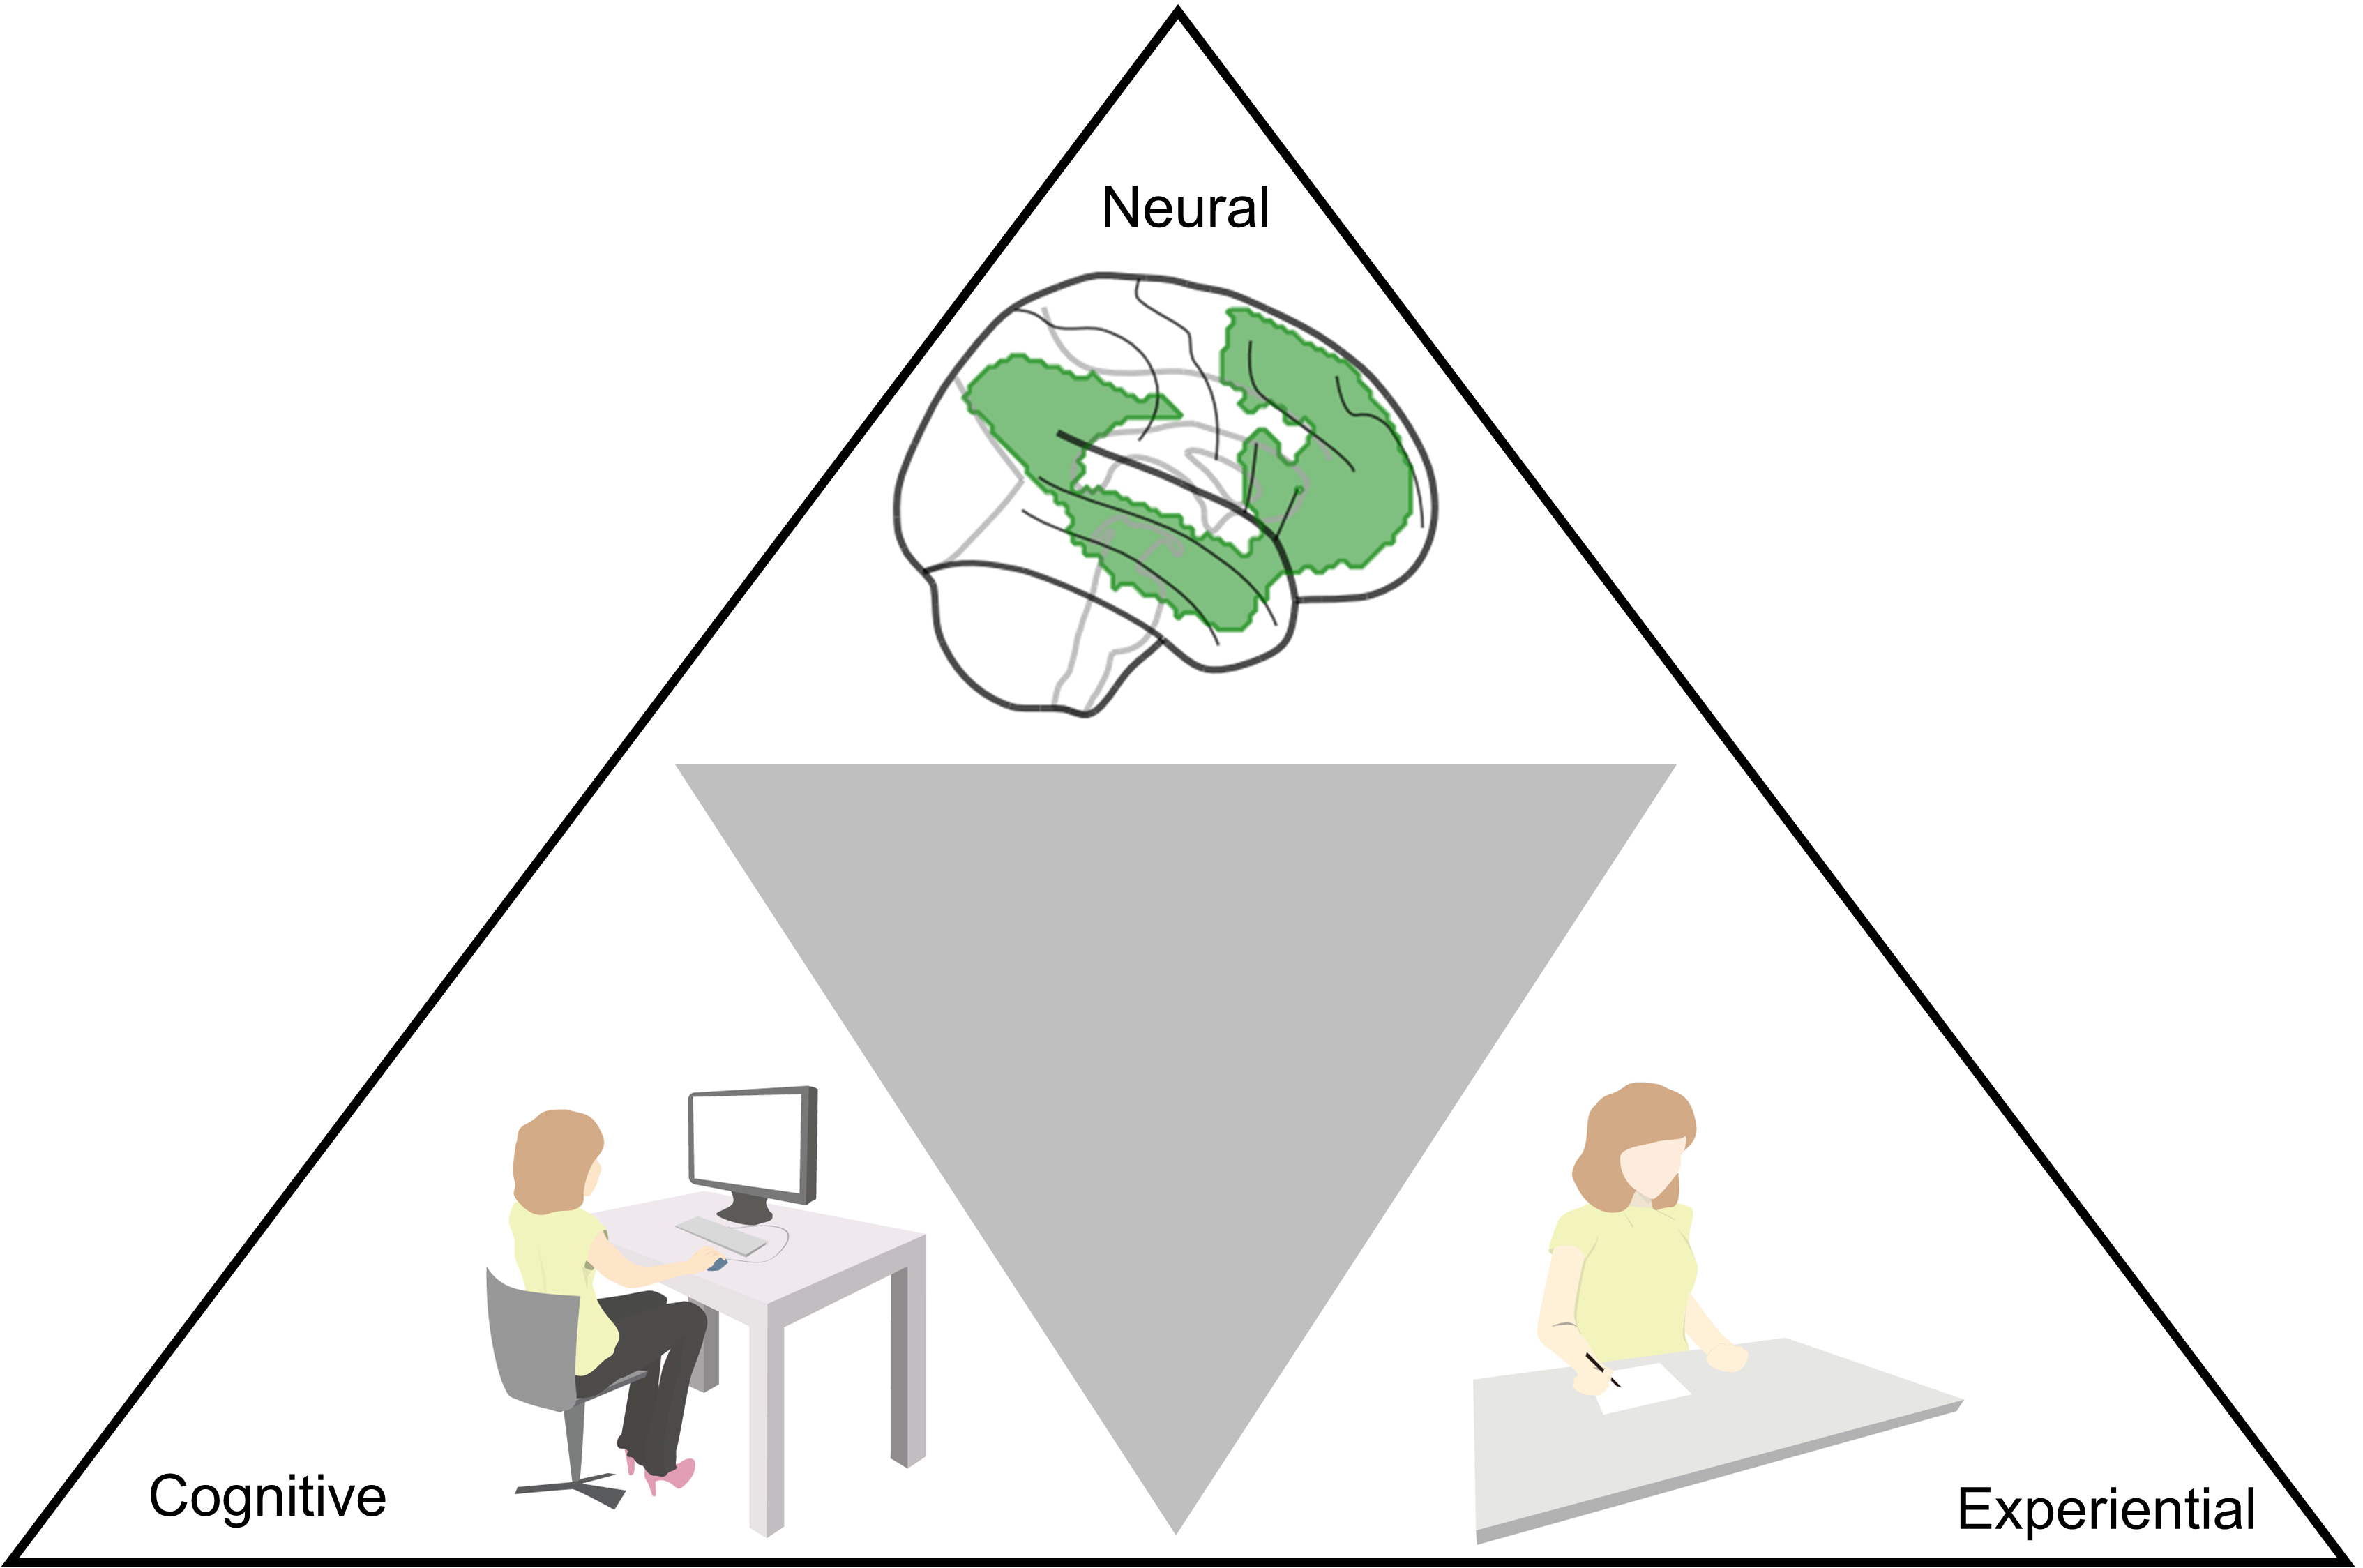
\includegraphics[width=0.6\textwidth]{chapters/img/thesisfig1.png}
	\caption{Schematic of the thesis}
	\label{fig:intro:fig1}
\end{figure}

\subsection{Content of experience}

To access the complex, heterogeneous content of spontaneous thoughts, the current thesis employs MDES \cite{Medea2016, RubyPlos2013, Smallwood2016}. For the purpose of capturing momentary evolution of thoughts during experiments, experience sampling \cite{Kahneman2004} is the commonly used technique. MDES expanded the thought probe from a on/off task question to a collection of dimensions related to a wide range of form and content of thoughts. The idea of MDES is based on various questionnaires to understand the content of mind wandering thoughts retrospectively, such as the Dundee Stress State Questionnaire \cite{Matthews1999}, Amsterdam Resting-State Questionnaire \cite{Diaz2013}, the resting state questionnaire \cite{Delamillieure2010}, and New York Cognition Questionnaire \cite{Gorgolewski2014}. The questionnaires above involves more than 20 items, providing a comprehensive coverage of thought content. Direct implementation of the retrospective questionnaires listed above is not practical for experience sampling. Experience sampling is conducted along an external task, such as reading \cite{Franklin2011}, go/no-go task \cite{Christoff2009}, and n-back task\cite{Kane2007}. The list of questions need to be short and concise to minimum interruption of the external task.

The current version of MDES is based on 10-question set used in \cite{Medea2016} and \citeA{Smallwood2016}. In the previous work, the questions are separated into content and form aspect of experience. Principle component analysis (PCA) was used to extract latent linear structure in the spontaneous thought report. Each participant has a set of identified principle components concluding the average momentary state of all the sampled time period. The current version includes both form and content questions in one set with three extra questions. The average score of each thought dimension indicate the average momentary state of spontaneous thought.

\subsection{Method of acquiring experience}

In the current thesis, both online and retrospective method are used to acquire content of mind wandering in laboratory scenario. In the second empirical study, New York Cognition Questionnaire \cite{Gorgolewski2014} is used to acquire the trait-like multidimensional mind wandering thought content during a 9-minute resting state fMRI session. The retrospective method measures the summary of the mind-wandering experience during a specified time period. The benefit of retrospective measure is that no interruption during the given task or the on-going thoughts will happen. The trait-level features of mind wandering are accessed in the retrospective report. 

In the online measure, MDES serves as the thought probes to record participant's experiences during a give task. A hybrid of go/no-go task and n-back task was used to manipulate working memory capacity to induce mind wandering \cite{Konishi2015, Medea2016}. The earlier version has used number as the test items \cite{SmallwoodNI2013}. The majority of the experiment consist of nontarget presented in neutral colour and a small proportion of targets. The participant are instructed to judge whether the target number is odd or even. In the \textit{choice reaction time} (i.e. 0-back) condition, the judgement is made when the number changes colour; in the \textit{working memory} (i.e. 1-back) condition, participants judge the number on the previous screen when presented with a question mark. The improved version is proposed by Konishi and colleagues \citeyear{Konishi2015}, replacing number with two 2-dimensional geometric shapes separated by a vertical line. Each pair consists of a two shapes among a circle, a triangle, and a square, each in two different left/right configurations. In the 0-back condition, the target is flanked by one of two shapes, and participants indicate which shape matches the target shape. In the 1-back condition, the target is flanked by two question marks, and participants match the target shape to the prior trial. Thought probe appears during the task in a semi random fashion. The online measure captures spontaneous thought in, possibly, both mind-wandering and task-focused moments. In the first and third empirical studies, the averaged momentary report from MDES is used to capture the trait-like feature of spontaneous cognition.

\subsection{Conjoined decomposition of brain and cognition}

Despite invented in the 30s, CCA has not aroused researchers’ interests due to the lack of practicality. With the advance on computing resource and enriched data size, CCA has gained popularity in neuroimaging research. Three characteristic of CCA make it the choice of method---joint information compression, symmetry, and multiplicity (details described in the Method chapter). CCA can be understood as a natural extension of PCA to two variable sets, but mutually linked by a joint correlation criterion. Such extension enables the exploration of neuro-experiential component pairs of mind wandering. CCA does not distinguish between the two variable sets during the information compression process. The identified dual-component dimensions correlates two aspect the data together without indication of causality between neural function and cognition. CCA is capable of estimating more than one corresponding component pair from the two variable sets. More than one pair of meaningful decomposition can be found, giving it the potential to examine the heterogeneity of mind wandering content and their functional outcome. 

While CCA provided useful features to explore the heterogeneity of mind wandering, its sparsity variation overcomes two technical issues of CCA application. Performing feature selection with sparsity improve the interpretability of the data and model fit. The data with more number of features than samples is accompanied with consequences of the so-called curse of dimensionality---the more dimensions are added to a data set, the less explanatory value a sample would have \cite{Domingos2012}. The number of functional connectivity measure can easily exceed the number of samples. In sum, SCCA allows decomposition on functional connectivity measures without sacrifice of data richness or interpretation difficulty of prior data compression. The pros and cons of CCA and its variation is disccussed in the next chapter.

The current thesis adopt the sparse variation of CCA \cite<SCCA; >{WittenSCCA2009} to resolve arguments related to heterogeneity in mind wandering. Most studies in mind wandering have only focused on its relationship with one cognitive outcome at a time. As a consequence, mind wandering is treated as a singular construct. Studies on contents of spontaneous thoughts have shown the diversity of information using self-report methods. Based on the heterogeneity of content of spontaneous thoughts, mind wandering can be a collection various type of spontaneous thoughts. Adopting multivariate method has the potential to identify family resemblance among the heterogeneity of mind wandering, and to begin the research on the ontological view of mind wandering. 
% ==========================================================================================================
\section{Summary}
In the current PhD, we would like to explore the numerous thoughts to describe human consciousness experience and establish a framework that incorporate the heterogeneity of the mind-wandering experience. The wide range of functional outcomes and contents of the mind-wandering state is perplexing as often time, those features are contradictory against each other. These studies indicated that the mind-wandering state is a heterogeneous collection of experiences that each type of the mind-wandering experiences has its own underlying cognitive mechanism and contextual representation (Smallwood \& Andrews-Hanna, 2013). The current difficulty of advancing the mind-wandering research is that, although the related cognitive and experience phenotypes has been found, we are unsure about the mechanism uniting those features. Moreover, the integrative nature of higher level cognition makes it difficult to identify the contribution of different processes to the mind-wandering state. This PhD aims to advance the understanding of the identified cognitive processes and find the quantifiable features of the cognitive measures that can infer the mind-wandering states. With the combination of MDES that accesses the heterogeneity of the content, cognitive phenotypes and the neuroimaging data, this PhD aims to establish the ontology of spontaneous thoughts and lays a solid foundation for future studies in consciousness. 
% ==========================================================================================================

\chapter{Canonical Correlation Analysis}
\label{ch:methods}
%\setcounter{equation}{0}


\textit{The following chapter has been adapted from:\\}
Wang, H.-T., Smallwood, J., Bassett, D. S., Satterthwaite, T.D. \& Bzdok, D. (2018). Finding the needle in many dimensions: A tutorial on CCA in biomedicine. Manuscript preparing for publication
\footnote{
D. Bzdok and H.-T. Wang planned the structure of the manuscript.  H.-T. Wang. drafted the manuscript under the supervision of D. Bzdok. All the authors approved the final version of the manuscript prior to submission.}\\
% ==========================================================================================================
\newpage
%Abstract

\noindent{}Nam auctor neque sed eros iaculis sit amet facilisis tellus tincidunt. Donec quis turpis a purus cursus porta. Nam vel massa nibh, a hendrerit libero. Mauris fringilla, arcu sed molestie cursus, nulla tortor aliquet nisi, et feugiat dui eros id ligula. Donec faucibus sodales nisl, quis interdum libero eleifend at. Sed turpis purus, fringilla quis porttitor id, pulvinar at metus. In hac habitasse platea dictumst. Integer lobortis sodales volutpat. Etiam iaculis euismod porta. Praesent quis venenatis massa. Cras laoreet posuere accumsan. Sed urna quam, laoreet sit amet hendrerit eu, tincidunt eu orci. Praesent eleifend diam sed metus eleifend sit amet volutpat dui interdum. Nam auctor neque sed eros iaculis sit amet facilisis tellus tincidunt. Donec quis turpis a purus cursus porta. Nam vel massa nibh, a hendrerit libero. Mauris fringilla, arcu sed molestie cursus, nulla tortor aliquet nisi, et feugiat dui eros id ligula. Donec faucibus sodales nisl, quis interdum libero eleifend at. Sed turpis purus, fringilla quis porttitor id, pulvinar at metus. In hac habitasse platea dictumst. Integer lobortis sodales volutpat. Etiam iaculis euismod porta. Praesent quis venenatis massa. Cras laoreet posuere accumsan. Sed urna quam, laoreet sit amet hendrerit eu, tincidunt eu orci. Praesent eleifend diam sed metus eleifend sit amet volutpat dui interdum.


% ==========================================================================================================

\section{Motivation}
\label{CCA:motivation}

% ==========================================================================================================

\section{Modelling intuitions}
\label{cca:intuitions}


% ==========================================================================================================

\section{Examples}
\label{cca:examples}


% ==========================================================================================================

\section{Interpretations}
\label{cca:interpretations}


% ==========================================================================================================

\section{Limitations}
\label{cca:limitations}


% ==========================================================================================================

\section{Relation to other commonly used methods}
\label{cca:other}


% ==========================================================================================================

\section{Practical considerations}
\label{cca:impliment}


% ==========================================================================================================
\chapter{Dimensions of Experience: Exploring the Heterogeneity of the Wandering Mind}
\chaptermark{Dimensions of Experience}
\label{ch:study1}
%\setcounter{equation}{0}
\textit{The following chapter has been adapted from:\\}
Wang, H.-T., Poerio, G. L., Murphy, C. E., Bzdok, D., Jefferies, E., \& Smallwood, J. (2018). Dimensions of Experience: Exploring the Heterogeneity of the Wandering Mind. \textit{Psychological Science}, \textit{29} (1), 56-–71. doi: 10.1177/0956797617728727
\footnote{
J. Smallwood, E. Jefferies, H.-T. Wang, and C. Murphy designed the study. H.-T. Wang, C. Murphy, and G. Poerio collected the data. The connection-strength and sparse canonical-correlation analysis pipeline was constructed by D. Bzdok and H.-T. Wang. Data were analyzed by H.-T. Wang, C. Murphy, and G. Poerio under the supervision of D. Bzdok, J. Smallwood, and E. Jefferies. H.-T. Wang and J. Smallwood drafted the manuscript. G. Poerio and D. Bzdok provided critical revisions. All the authors approved the final version of the manuscript prior to submission.
}\\

%Abstract
\newpage
\noindent{}The tendency for the mind to wander to concerns other than the task at hand is a fundamental feature of human cognition, yet the consequences of variations in its experiential content for psychological functioning are not well understood. Here, we adopted multivariate pattern analysis to simultaneously decompose experience-sampling data and neural functional-connectivity data, which revealed dimensions that simultaneously describe individual variation in self-reported experience and default-mode-network connectivity. We identified dimensions corresponding to traits of positive-habitual thoughts and spontaneous task-unrelated thoughts. These dimensions were uniquely related to aspects of cognition, such as executive control and the ability to generate information in a creative fashion, and independently distinguished well-being measures. These data provide the most convincing evidence to date for an ontological view of the mind-wandering state as encompassing a broad range of different experiences and show that this heterogeneity underlies mind wandering's complex relationship to psychological functioning.
% ==========================================================================================================

\section{Introduction}
\label{study1:intro}
Although people's minds frequently wander from events in the here and now, or any task being performed, the functional consequences of this state remain poorly understood \cite{Mittner2016,Seli2016,Smallwood2013d}.
Some studies link mind wandering to unhappiness
\cite{Killingsworth2010}; 
others suggest it facilitates recovery from negative emotional states
\cite{Poerio2016,Ruby2013a}.
Mind wandering is associated with poorer performance on tasks that place high demands on executive functions
\cite{McVay2009,Mrazek2012},
yet studies of problem solving suggest that mind wandering may promote creativity 
\cite{Baird2012,Smeekens2016}.
This wide range of associated functional outcomes is puzzling--—if mind wandering is a homogeneous construct, then it is unclear why it should be associated with such a complex array of often opposing outcomes. To reconcile this contradictory evidence, researchers have suggested that mind wandering may be heterogeneous, encompassing multiple states with differential contents and underlying cognitive architectures \cite{Smallwood2013d}. According to this ontological perspective, different functional associations arise from different “types” of experience, which explains the range of functional outcomes observed in the literature.

In the current study, we recruited 165 participants and obtained data on (a) the organization of the brain at rest using functional MRI (fMRI), (b) the content and form of experience recorded across different days, (c) cognitive functions assessed by a comprehensive battery of tasks (including memory, creativity, and executive control), and (d) psychological well-being via questionnaires. Our procedure is presented in Figure \ref{fig:study1:fig1}. These data allowed us to use novel multivariate analysis methods to test the hypothesis that there are different types of mind wandering, with unique neural and experiential patterns accounting for unique variance in the psychological profile of our sample.

\begin{sidewaysfigure}[p]
	\centering
	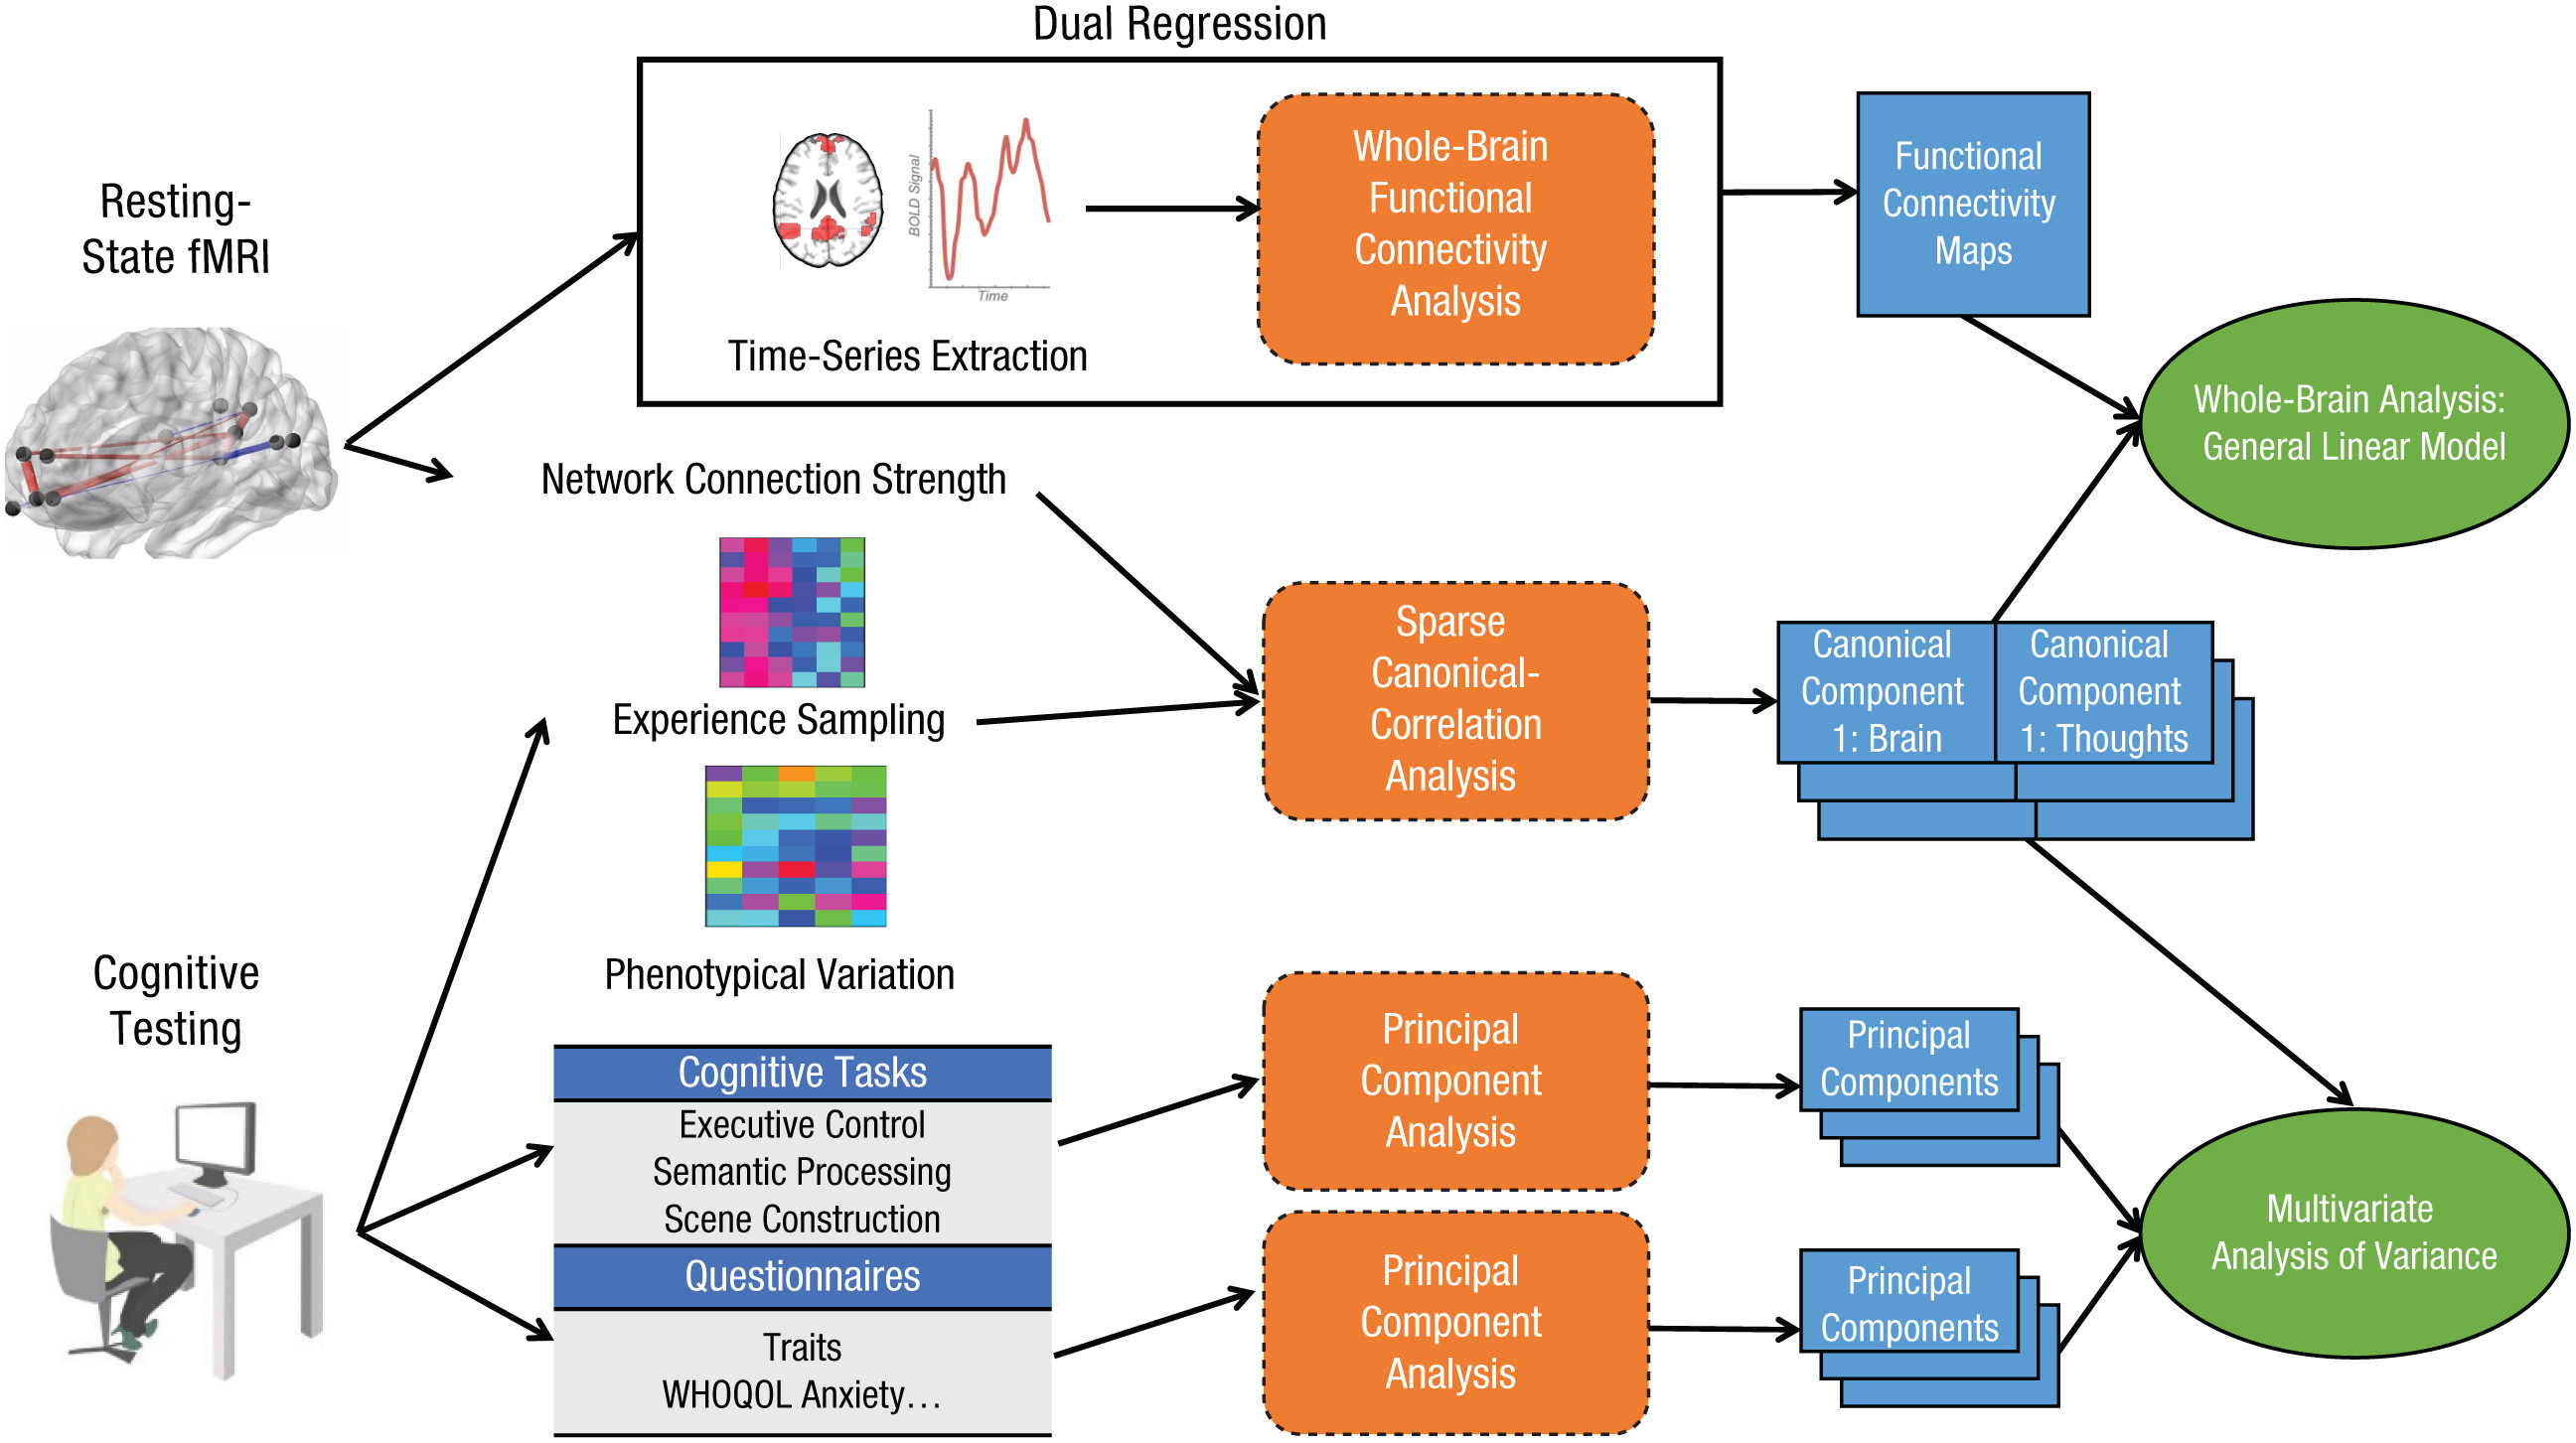
\includegraphics[width=0.8\textwidth]{chapters/img/study1fig1.jpeg}
		\caption{Schematic of the procedure and analysis strategy employed in the current study.}
		\caption*{We collected resting-state functional MRI (fMRI) data, cognitive-function measures, and questionnaires on personal traits for each participant. These were submitted to analysis (rectangles with dashed borders), which created latent components or features (rectangles with solid borders) for each subject, and these variables were subsequently passed to the main analysis (ovals). WHOQOL = World Health Organization Quality of Life assessment \cite{WHOQOL2002}.}
		
	\label{fig:study1:fig1}
\end{sidewaysfigure}

We used functional connection strength to characterize the neural organization of each individual. We selected regions for our analysis on the basis of evidence that task-unrelated thoughts are linked to concurrent increases in activity in medial prefrontal cortex (mPFC), posterior cingulate cortex (pCC), and lateral parietal cortex
\cite<for meta-analyses, see>{Fox2015,Stawarczyk2015}.
—regions that make up the core of the default mode network
\cite<DMN;>{Buckner2008}.
During mind wandering, it is believed that these regions interact with other areas of the cortex, in particular, temporal lobe regions associated with memory representation that are also allied to the DMN. For example, the hippocampus activates early during mind wandering
\cite{Ellamil2016}. 
whereas connectivity between lateral and medial aspects of the temporal lobe and the DMN core predicts individual variation in features of mind wandering, such as its episodic content
\cite{Karapanagiotidis2017}. 
Contemporary accounts of mind wandering posit that the DMN may be important for automatic aspects of cognition
\cite{Christoff2016}. 
Other studies have highlighted links with the lateral prefrontal cortex, which is important for executive control when mind wandering is more deliberate \cite<e.g.,>{Golchert2017}.

We applied multivariate pattern analysis to the neurocognitive and experiential data to identify different types of mind wandering. If the DMN is important for automatic aspects of cognition \cite{Christoff2016}, states linked to high levels of connectivity within this system may have experiential features reflecting more automatic types of cognition. Our a priori decision to focus on the DMN core to derive patterns of experience limited our ability to observe interactions with regions outside of this system, so we used whole-brain functional connectivity to characterize these links for each type of experience. On the basis of prior studies \cite<e.g.,>{Ellamil2016,Golchert2017,Smallwood2016}, we expected this analysis to identify connections with regions in the temporal lobe or the executive system. This pattern would confirm the hypothesized accounts of the DMN as important in integrating neural information \cite{Margulies2016,Smallwood2016}. Having characterized different types of mind wandering in both brain and experience, we used these to test the hypothesis that different categories of experience are related to different functional outcomes. We performed an individual differences analysis to understand whether our characterized types of mind wandering have unique functional associations, including better creativity, worse executive control, and lower levels of well-being. We expected different patterns of experience to capture different psychological profiles explaining the heterogeneous pattern of functional outcomes that have been linked to the mind wandering state in previous studies
\cite{Smallwood2013a}.

% ==========================================================================================================

\section{Method}
\label{study1:method}
\subsection{Participants}
\label{study1:method:a}
One hundred sixty-five healthy participants were recruited from the University of York (99 females, 66 males; age range = 18--31 years, \textit{M} = 20.43, \textit{SD} = 2.63). We preselected a sample size approximately double those used in our prior studies \cite<e.g.>{Smallwood2016}.%(e.g., Smallwood et al., 2016). 
A sample size of at least 125 is recommended in order to have 95\% confidence that a correlation of typical size (\textit{r} = .20--.30) is present and greater than 0
\cite{Hemphill2003}.
Participants were right-handed native English speakers with normal or corrected-to-normal vision and no history of psychiatric or neurological illness. Participants underwent MRI scanning, completed an online questionnaire, and then attended three 2-hr behavioral testing sessions to complete a battery of cognitive tasks. The behavioral sessions took place within a week of the scan. Eight participants were excluded from the multivariate pattern analysis because they failed to complete all of the behavioral testing sessions. In total, 157 participants were included in the multivariate pattern analysis and the comparison with cognitive performance. One hundred forty-two participants completed both the behavioral testing sessions and questionnaires and were included in the analysis associated with well-being. Participants were rewarded with either a payment of \pounds 80 or a commensurate amount of course credit. All participants provided written consent prior to the fMRI session and the first behavioral testing session. Approval for the study was obtained from the ethics committee of the University of York Department of Psychology and the University of York Neuroimaging Centre.

\subsection{MRI acquisition}
\label{study1:method:b}
Structural and functional data were acquired using a 3T HDx Excite MRI scanner (GE Healthcare, Little Chalfont, United Kingdom) utilizing an eight-channel phased-array head coil tuned to 127.4 MHz at the York Neuroimaging Centre, University of York. Structural MRI acquisition in all participants was based on a T1-weighted 3-D fast-spoiled gradient-echo sequence— repetition time (TR) = 7.8 s, 
echo time (TE) = minimum full, 
flip angle = \ang{20}, 
matrix size = 256 $\times$ 256, 176 slices, 
voxel size = \SI[product-units=power]{1.13 x 1.13 x 1}{\mm}.
Resting-state activity was recorded from the whole brain using single-shot 2-D gradient-echo-planar imaging—TR = 3 s, TE = minimum full, 
flip angle = \ang{90}, 
matrix size = 64 $\times$ 64, 60 slices, 
voxel size = \SI[product-units=power]{3 x 3 x 3}{\mm}, 180 volumes. 
Participants viewed a fixation cross for the duration of the 9-min fMRI resting-state scan. A fluid-attenuated inversion-recovery (FLAIR) scan with the same orientation as the functional scans was collected to improve co-registration between subject-specific structural and functional scans.


\subsection{Questionnaires}
\label{study1:method:c}
We administered a battery of questionnaires to comprehensively assess a diverse range of trait-level individual differences that have been previously related to mind wandering. These questionnaires captured the trait-like features of participants’ psychological states, particularly aspects of well-being. The complete details of the questionnaires are presented in Appendix \ref{appendix:study1:subsection1}.

\subsection{Behavioral testing sessions}
\label{study1:method:d}
The trait profiles captured by the questionnaires were complemented by measures of performance on a range of cognitive tasks. Behavioral tasks were selected to measure a broad range of cognitive attributes, including semantic and episodic memory, executive control, fluency, and creativity. These measures were assessed in three sessions. Each session began with a task to index the content and form of mind wandering (0-back/ 1-back task), followed by the other cognitive measures. The order of sessions and the order of tasks was counterbalanced across individuals. Details of the 0-back/ 1-back task are presented in the following paragraph. The complete details of the other cognitive tasks are described in Appendix \ref{appendix:study1:subsection2}.
Using a block design, we assessed the contents of experience during mind wandering in the context of a simple task that manipulated working memory load
\cite<see>[for prior published examples of this task]{Konishi2015,Medea2016}.
This task was performed at the beginning of each laboratory session to minimize participant fatigue. Measuring experience over 3 days provided us with a more comprehensive description of participants’ trait-level mind wandering than would have been possible in a single experimental session.
In both tasks, participants completed target and nontarget trials. In nontarget trials, a pair of shapes appeared on screen; the two shapes were separated by a vertical line. The pairs consisted of a circle and a square, a circle and a triangle, and a square and a triangle, each in two different left/right configurations for a total of six possible pairs. Following an unpredictable sequence of nontarget trials, a target trial was presented in which participants had to make a manual response. The target was a small stimulus presented in either blue or red across conditions, with the color counterbalanced across participants. In the 0-back condition, the target was flanked by one of two shapes, and participants had to indicate which shape matched the target shape by pressing the appropriate button. In the 1-back condition, the target was flanked by two question marks, and participants had to respond depending on which side the target shape had been on during the prior trial. Responses were made using the left and right arrow keys. Presentation times for fixation crosses ranged from 1.3 to 1.7 s in steps of 0.05 s, and nontarget presentation times varied from 0.8 to 1.2 s in steps of 0.05 s. Target presentation times always ranged from 2.1 to 2.5 s in steps of 0.05 s, and a response from participants did not end the target presentation.
There were eight blocks in one session, and each block consisted of two to four miniblocks. Each block contained either the 0-back or 1-back condition. The change of task was signaled by the presentation of the word “SWITCH,” which remained on screen for 5 s. The order of the tasks was counterbalanced across participants, and the eight blocks lasted around 25 min. In each mini-block, there was one target trial, and the number of nontarget trials preceding the targets varied between one and six. Participants’ performance was measured by their efficiency, which was calculated by dividing their average response time by their accuracy. For ease of interpretation, efficiency scores were reversed, so that higher scores indicated better performance.
In order to sample different features of participants’ ongoing experiences, we used multidimensional experience sampling
\cite<MDES;>{Medea2016,Ruby2013a,Smallwood2016}. 
This technique uses self-report data to assess the contents of experience on a number of dimensions. The first thought probe asked participants to rate their level of task focus (“My thoughts were focused on the task I was performing”) on a sliding scale from 0 (completely off task) to 1 (completely on task). Participants then answered 12 randomly presented questions regarding the content and form of their experience at the moment just before they answered the first thought probe (on level of task focus). These questions (described in Table \ref{tab:study1:1}) were based on those used in prior studies adopting this approach to measure self-generated thought
\cite{Medea2016,Ruby2013a,Smallwood2016}.  
At the moment of target presentation, there was a 20\% chance of a thought probe being presented instead of a target, with a maximum of one probe per block of the 0-back/1-back task. In each session, an average of 14.07 (SD = 3.30, range = 6–25) MDES probes occurred; in the 0-back condition, an average of 7.02 (SD = 2.36, range = 2–14) MDES probes occurred; and in the 1-back condition, an average of 7.04 (SD = 2.24, range = 1–15) occurred. In total, we sampled 7,006 examples of experience in this study. We calculated the mean scores of each question across the three sessions for each participant. The MDES scores were first transformed into z scores for mean-centering and univariance scaling. The scores described the average momentary experience in each dimension. We used this score in the multivariate analysis later.

\linespacesmall
\begin{table}
\centering
\caption{Experience-Sampling Questions in the 0-Back/1-Back Task.}
\label{tab:study1:1}
\resizebox{\textwidth}{!}{
\begin{tabular}{ l l c c}
\toprule
& & \multicolumn{2}{c}{Response scale} \\ \cmidrule{3-4}
Dimension & \multicolumn{1}{c}{Question} & 0 & 1 \\ \midrule
Focus & My thoughts were focused on the task I was performing.  & \textit{Not at all} & \textit{Completely} \\
Future & My thoughts involved future events. & \textit{Not at all} & \textit{Completely} \\
Past & My thoughts involved past events. & \textit{Not at all} & \textit{Completely} \\
Self & My thoughts involved myself. & \textit{Not at all} & \textit{Completely} \\ 
Other & My thoughts involved other people. & \textit{Not at all} & \textit{Completely} \\
Emotion & The content of my thoughts was: & \textit{Negative} & \textit{Positive} \\ 
Images & My thoughts were in the form of images. & \textit{Not at all} & \textit{Completely} \\
Words & My thoughts were in the form of words. & \textit{Not at all} & \textit{Completely} \\
Vividness & My thoughts were vivid as if I was there. & \textit{Not at all} & \textit{Completely} \\
Detail & My thoughts were detailed and specific. & \textit{Not at all} & \textit{Completely} \\
Habit & This thought has recurrent themes similar to those I have had before. & \textit{Not at all} & \textit{Completely} \\
Evolving & My thoughts tended to evolve in a series of steps. & \textit{Not at all} & \textit{Completely} \\
Deliberation & My thoughts were: & \textit{Spontaneous} & \textit{Deliberate} \\ \bottomrule
\end{tabular}
}
\end{table}
\linespacenormal

\subsection{Neuroimaging data preprocessing and analysis}
\label{study1:method:e}
\subsubsection{Resting-state fMRI.} 
Functional and structural data were preprocessed and analyzed using the Oxford Centre for Functional MRI of the Brain’s (FMRIB’s) Software Library (FSL Version 4.1, www.fmrib.ox.ac.uk/fsl). Individual FLAIR and T1-weighted structural brain images were extracted using FSL’s Brain Extraction Tool (BET). Structural images were linearly registered to the MNI152 template using FMRIB’s Linear Image Registration Tool (FLIRT). The resting-state functional data were preprocessed and analyzed using FSL’s FMRI Expert Analysis Tool (FEAT). The individual-subject analysis involved motion correction using FSL’s MCFLIRT, slice-timing correction using Fourierspace time-series phase shifting, high-pass temporal filtering (Gaussian-weighted least-squares straight-line fitting, $\sigma$= 200 s), and Gaussian low-pass temporal filtering ($\sigma$ = 2.8 s). In addition, we regressed out six motion parameters (as estimated by MCFLIRT) and regressing out cerebrospinal fluid and white-matter signal (top five components in the principal component analysis, PCA; CompCor method). No spatial smoothing and no global signal regression were applied.

\subsubsection{Network-strength analysis.} To describe the functional architecture of the DMN, we transformed the resting-state blood-oxygen-level-dependent time series into connection strength values of the selected regions for each participant. The regions of interest (ROIs) were obtained from connectivity-based functional parcellation studies of the DMN by Bzdok and colleagues
\cite{Bzdok2013,Bzdok2015,Bzdok2016,Eickhoff2016,Eickhoff2016}.
There were 16 selected target network nodes, including subregions located in the bilateral temporoparietal junction (TPJ), ventromedial prefrontal cortex (vmPFC), dorsomedial prefrontal cortex (dmPFC), and posteromedial cortex 
(PMC; see Fig.\ref{fig:study1:fig2}a). 
The ROI masks and the related functional-connectivity network produced with Neurosynth core tools 
(\url{https://github.com/neurosynth/neuro\_synth}) 
can be found on NeuroVault 
(\url{http://neurovault.org/collections/2275/}). First, we extracted and then averaged the time series of all voxels within the 6-mm sphere masks of the given regions. Second, we created 16 $\times$ 16 symmetrical correlation matrices representing the network of the regions that was computed for all the individual subjects. The off-diagonal of each correlation matrix contained 120 unique region-region connection strengths. This approach provided a measure of connection strength of the region-region coupling of the DMN for each participant.

\begin{sidewaysfigure}[p]
	\centering
	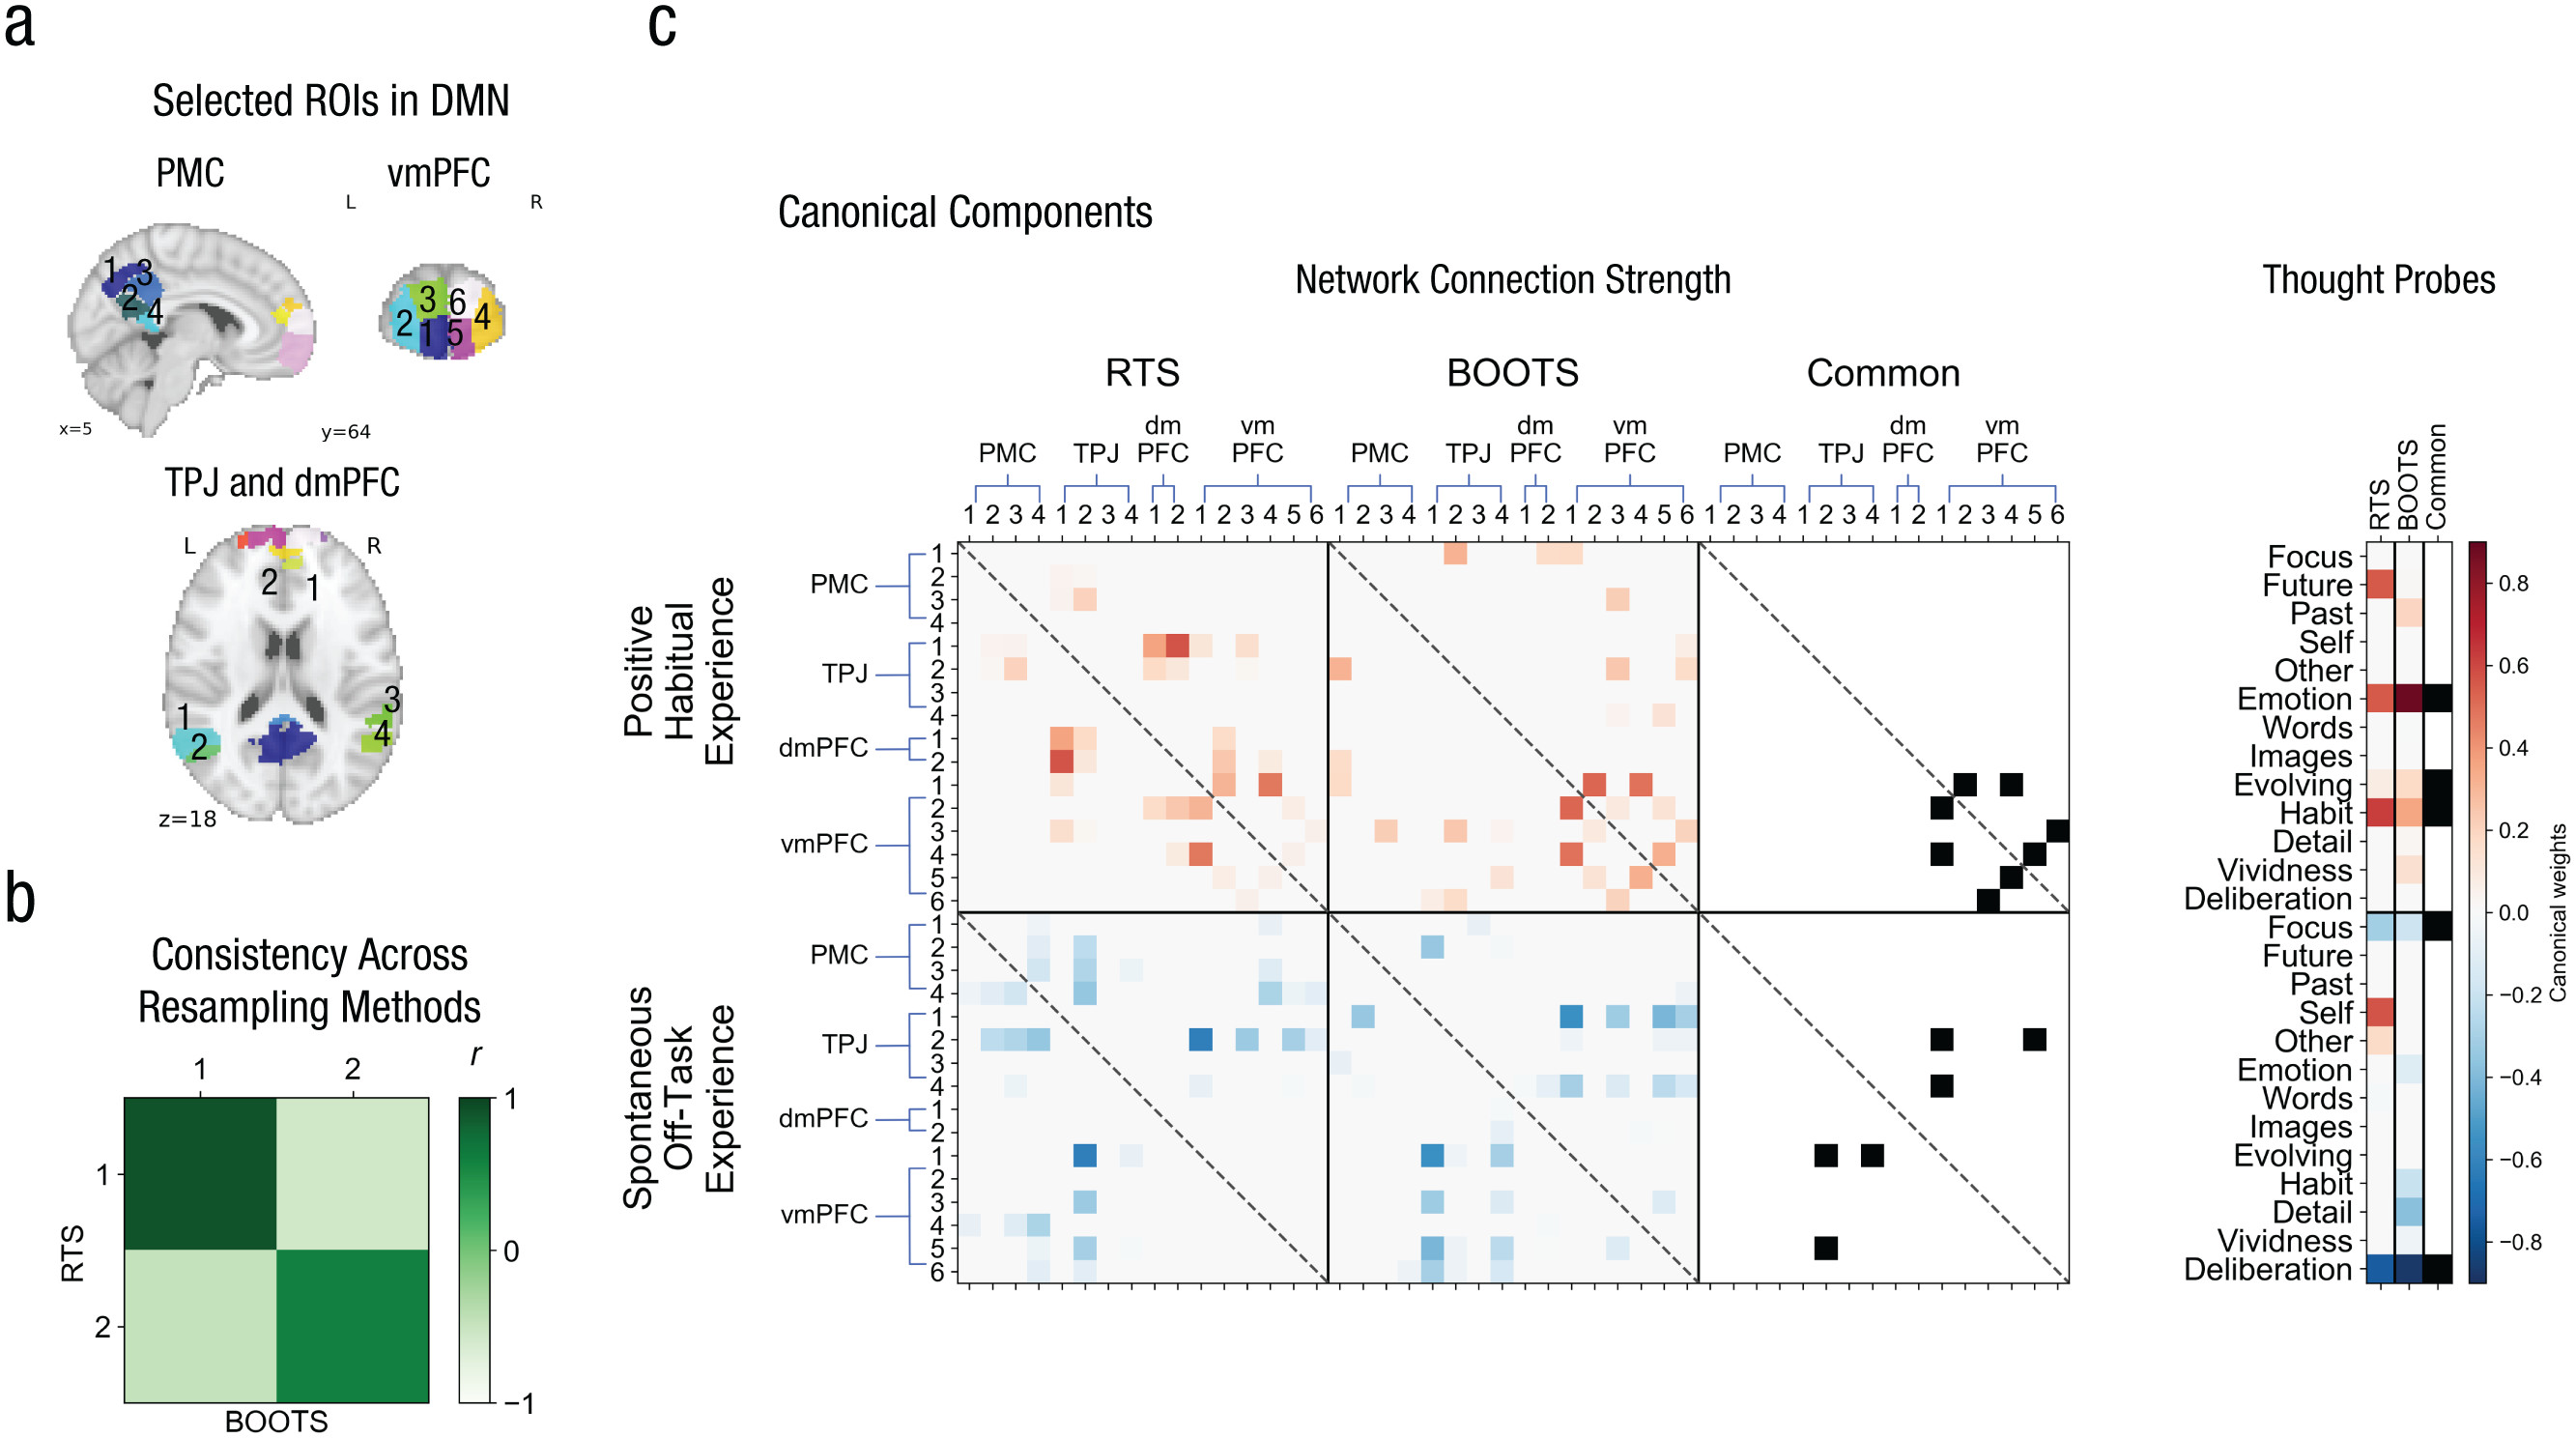
\includegraphics[width=0.8\textwidth]{chapters/img/study1fig2.jpeg}
	\caption{Results of the sparse canonical-correlation analysis.}
	\caption*{\scriptsize{The regions of interest (ROIs) of the default mode network (DMN) from which the network connection strength was calculated are shown in (a). The correlation between the two canonical components (positive-habitual experience, 1, and spontaneous off-task experience, 2) and the two analyses is shown in (b). The analyses were restricted temporal sampling (RTS), which describes the canonical components produced when the data from 1 day of each participant were randomly removed from the decomposition, and bootstrapping (BOOTS), which describes the solution produced using bootstrapping. Panel (c) shows the results of the sparse canonical-correlation analysis (SCCA) conducted on the network-connection-strength values of key nodes of the DMN at rest and self-reports of experience during a laboratory task. Results are shown separately for the two components of experience for each analysis. Also shown are the common findings between the two analyses. The numbers indicate the subregions of each ROI, as indicated in (a). For the questions associated with each self-report dimension, see Table 1. PMC = posteromedial cortex, vmPFC = ventromedial prefrontal cortex, TPJ = temporoparietal junction, dmPFC = dorsomedial prefrontal cortex.}}
	
	\label{fig:study1:fig2}
\end{sidewaysfigure}

\subsubsection{Multivariate pattern analysis.} We performed a sparse canonical-correlation analysis (SCCA) on the connection strength data and MDES scores to yield different dimensions that simultaneously described neural organization and experience. Canonical-correlation analysis (CCA) is an advanced multivariate technique that identifies distinct components between two variables spaces \cite{Hardoon2004}—in our case, brain-region connection-strength values and experiential reports obtained through MDES. This modeling approach allows linear combinations of the two variable vectors with correlations among variables to be determined and, unlike in PCA and independent component analysis, produces dimensions in which the biological data are simultaneously constrained by psychological measures (and vice versa). To enhance the interpretability of the decomposition solutions, we used a variant of CCA penalized by L1 regularization, SCCA \cite<see>{Hastie2015}. This was achieved by setting a maximum number of brain or behavior variables to exactly zero, which resulted in a regularized version of the singular value decomposition. A reliable and robust implementation of the SCCA method was retrieved as an R package from CRAN (penalized multivariate analysis, or PMA). In the current analysis, the L1 penalty was set to 0.3 on resting-state functional connectivity and to 0.5 for the MDES results. Other parameters were set to the default. In this way, our analysis performed low-rank (i.e., described an overall network pattern by a parsimonious set of connectivity causes), conjoint (i.e., respected variance in brain and behavior at once), and sparse (i.e., automatically found unimportant variables) decomposition of experiential and neural data.

\subsubsection{Stability analyses.} We performed two analyses to assess the stability of the solutions produced by SCCA. First, for each participant, we excluded the MDES data of 1 random day and then recalculated the average scores for these questions. We repeated the decomposition on this new set of MDES data and the network connection strength. This corroborative quantitative assessment provided insight into the robustness of the obtained findings by a permutation analysis that left 1 day out at a time. In particular, this procedure addressed whether either the first day (when participants may be learning how to respond to the experience-sampling method) or the last day (when participants may have lower levels of motivation) might unduly bias the decomposition solutions. We reasoned that if the average momentary MDES responses are stable across three sessions, then they should yield similar latent components. Second, we acquired bootstrap samples as a permutation analysis to estimate the variance and generalizability of the sample to the population. The bootstrap resamples, each reflecting an alternative data sample that we could have obtained from the same distribution, was created by random sampling with replacement. The identical SCCA computation was then reiterated individually on each of the 1,000 perturbed versions of the actual data sample. This approach enables quantitative assessment of the quality of the original SCCA estimates by inferring confidence intervals (see Fig.\ref{fig:3S1} in the Appendix \ref{appendix:study1:subsection3} for the distributions). We selected latent components that were consistent across the decomposition of the original sample, a leave-1-day-out sample, and a bootstrap sample, as those are the stable components that were less biased by the session effect and closer to our best estimation of population. We formalized the similarity of these two types of resampling by conducting a formal conjunction of the solutions generated through these different methods of resampling. To quantify the similarity between the components, we performed a conjunction that highlights the common elements of each solution. The feature conjunctions were calculated as follows:
% equation here
where LODO refers to leave 1 day out and BOOTS refers to bootstrapping. In addition, because bootstrapping produces a population estimation of our sample, we used the latent component weights produced by this method to compute component scores. This set of scores was used in all subsequent analyses. The source code for this analysis is available at \url{https://github.com/ htwangtw/DimensionsOfExperience}.

\subsubsection{Whole-brain analysis.} A limitation in our analysis is that we focused on the DMN to describe patterns of thought. To overcome this limitation, we generalized the types of experience provided by the SCCA by assessing their associations with areas outside of the DMN using a process conceptually similar to dual regression \cite{Beckmann2009}. To perform these analyses, we preprocessed and analyzed the resting-state functional data using FEAT. For the individual-subject preprocessing procedure, see the Resting-State fMRI section.
Following these preprocessing steps, we used a mask produced by the average of the DMN ROIs to determine the time series that described this neural system. This time series was used in a whole-brain functionality analysis for each participant. This allowed us to produce a subject-specific spatial map based on the selected ROIs, and these maps were used as dependent measures in our group-level analysis. To test whether the functional connectivity of the DMN ROIs was associated with the canonical components, we conducted a group-level analysis using FMRIB’s Local Analysis of Mixed Effects Stage 1 (FLAME 1). To control for spurious correlations that might emerge from movement, we included the two canonical components on thought reports only, group mean and Jenkinson’s mean framewise displacement \cite<FD>{Jenkinson2002}, as explanatory variables in the full model. The Jenkinson’s mean FD was calculated by the motion power statistic function in Configurable Pipeline for the Analysis of Connectomes 
(C-PAC; \url{https://fcp-indi .github.io/}). 
A 50\% probabilistic gray-matter mask was applied to the results maps, and the results were thresholded at the whole-brain level using cluster-based Gaussian random-field theory, with a cluster-forming threshold (Z) of 2.6 and a familywise-error-corrected cluster significance level (p) of .05. Unthresholded maps were uploaded onto Neurovault 
(\url{http://neurovault.org/images/43189/}).

\subsubsection{PCA.} To summarize the questionnaire and task data, we performed an initial data-reduction step using PCA in SPSS (Version 24). This analysis was performed separately for the questionnaires and task measures. One hundred forty-five participants’ data were included in the analysis of the questionnaire items, and 157 participants’ data were included in the analysis of the behavioral tasks. The behavioral-task measures were converted into z scores to avoid data distortions derived from the difference in score means. Missing data were imputed by mean scores in both analyses. The Kaiser-Meyer-Olkin (KMO) measure and Bartlett’s test of sphericity were used to measure the sampling adequacy of the model. Components were selected on the basis of the elbow in a scree plot (see Fig.\ref{fig:3S2} in Appendix \ref{appendix:study1:subsection3}), and varimax rotation was used to maximize the distinctiveness of each solution.
In the PCA of the phenotypical variation measured by behavioral tasks, Bartlett’s test of sphericity was significant, 
$\chi^{2}$(210) = 775.01, 
p < .001, which indicates that it is appropriate to apply PCA to these data. The KMO measure of sampling adequacy indicated that the current sample was acceptable for PCA (KMO = 0.79). The PCA of task performance revealed three principal components with a clear elbow after the third component observed in the scree plot. The three orthogonal components accounted for 40.7\% of the total variance; the component loading patterns are shown in Figure \ref{fig:study1:fig3}a. The three components, which accounted for 24.9\%, 8.3\%, and 7.5\% of the variance, respectively, can be interpreted as the three aspects of cognitive functioning: (a) semantic memory, (b) executive control, and (c) the generation of information (including letter or category fluency and the generation of creative solutions).
In the PCA of the questionnaire data, Bartlett’s test of sphericity was significant,
$\chi^{2}$(105) = 919.78, 
p < .001, which indicates that PCA is an appropriate model for the data. The KMO measure of sampling adequacy indicated that there were strong relationships among the variables (KMO = 0.82). The application of PCA to the questionnaire data revealed four components with a clear elbow after the fourth component observed in the scree plot in Fig. S2. The four orthogonal components accounted for 65\% of the total variance (produced component loading patterns are shown in Figure \ref{fig:study1:fig3}b). The four components accounted for 35\%, 14\%, 9\%, and 7\% of the variance, respectively. The first component, affective disturbance, was anchored at one end by high levels of depression and rumination and at the other by high levels of well-being. The second component was associated with high scores on four of the five autism subscales, excluding the attention-to-detail subscale. The third component loaded on components of both attention-deficit/hyperactivity disorder (ADHD) and dyslexia. The fourth component loaded on trait anxiety and high levels of attention to detail, as measured by the Autism Spectrum Quotient \cite{Baron-Cohen2001}. We analyzed these data using a multivariate analysis of variance (MANOVA) in which the dependent variables were the PCA loadings produced by the decomposition of the questionnaires, and the independent variables were the canonical component loadings.
\begin{figure}[p]
	\centering
	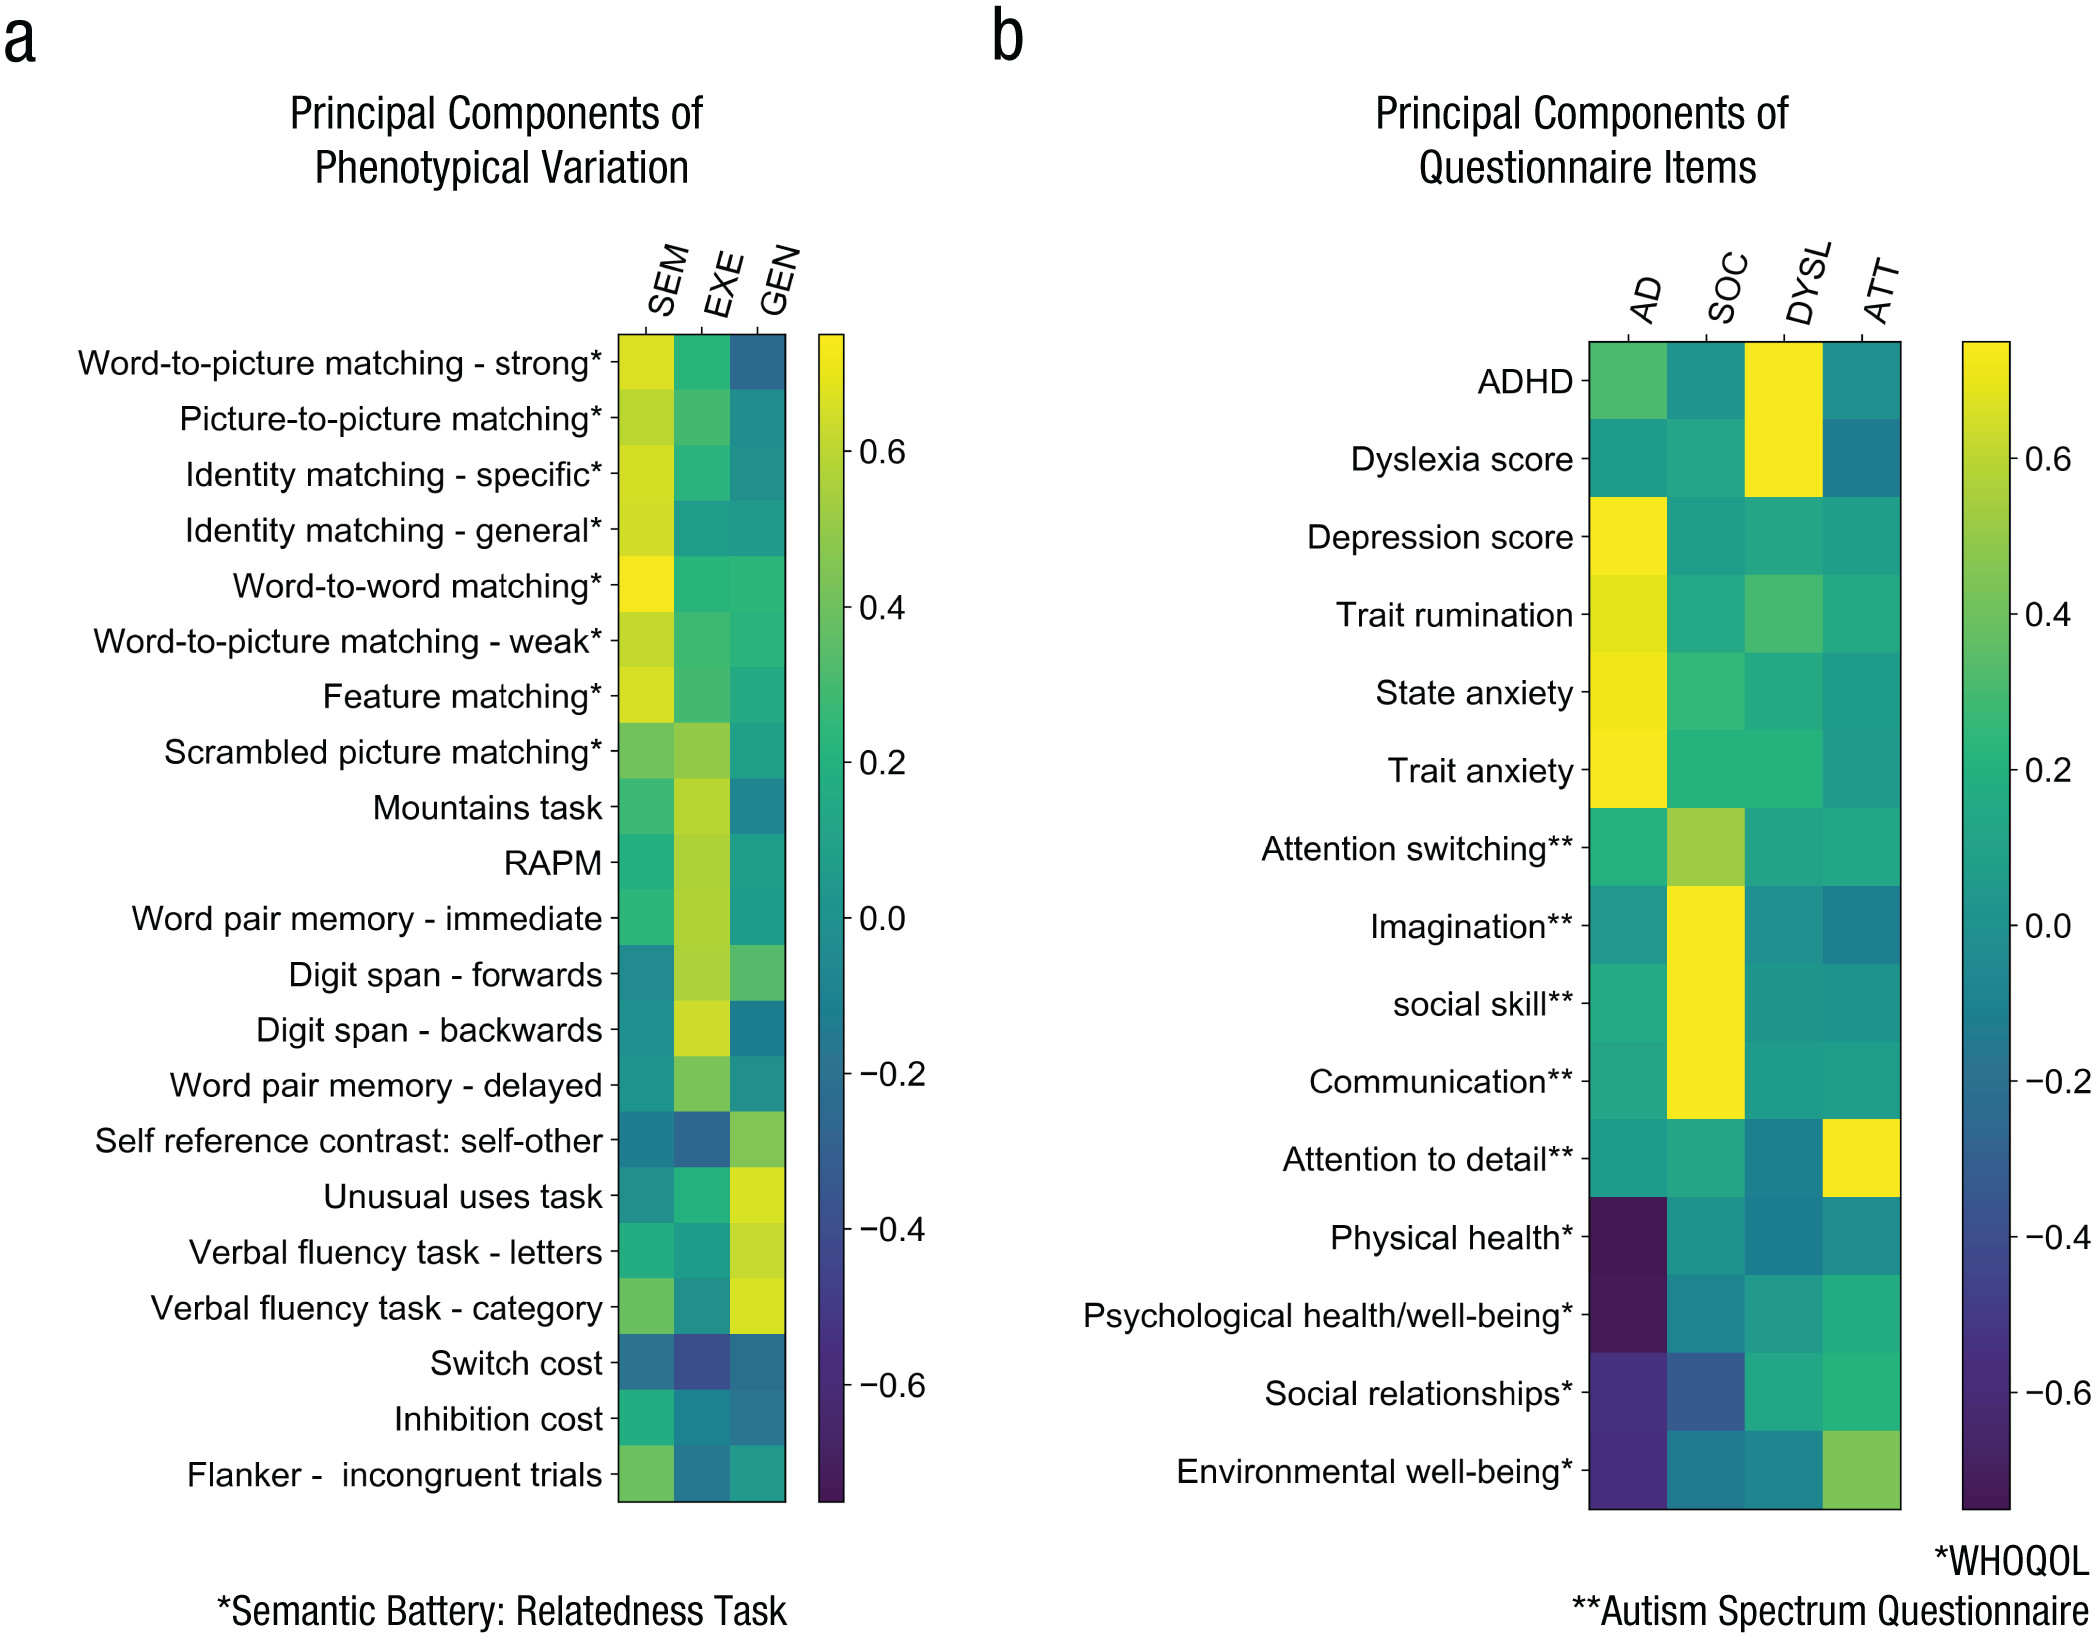
\includegraphics[width=0.8\textwidth]{chapters/img/study1fig3.jpeg}
	\caption{Results from principal component analyses of (a) behavioral tasks and (b) questionnaires.} 
	\caption*{In the analysis of behavioral tasks, the components were semantic memory (SEM), executive control (EXE), and the generation of information (GEN). In the analysis of questionnaire data, the components were affective disturbance (AD), social interaction (SOC), dyslexia (DYSL), and attention to detail (ATT). The heat map indicates the loadings of each measure. In (a), an asterisk indicates that measures were relatedness tasks from a semantic battery. In (b), a single asterisk indicates measures drawn from the World Health Organization Quality of Life assessment \cite{WHOQOL2002}, and two asterisks indicate measures drawn from the Autism Spectrum Quotient \cite{Baron-Cohen2001}. ADHD = attention-deficit/hyperactivity disorder; RAPM = Raven’s Advanced Progressive Matrices \cite{Raven1998}. For the scree plots describing the eigenvalues for each dimension, refer to Fig.\ref{fig:3S2} in Appendix \ref{appendix:study1:subsection3}.}
	\label{fig:study1:fig3}
\end{figure}
% ==========================================================================================================

\section{Results}
\label{study1:results}

\subsection{Determining consistent categories of experience}
\label{study1:results:a}
We applied SCCA to the network-connection-strength values among ROIs in the DMN and the average scores on the experiential reports gained in the laboratory. We accepted 13 canonical components generated by SCCA (see Fig.\ref{fig:3S3} in the Appendix \ref{appendix:study1:subsection3} for the complete set). Of these initial components, two were consistent when we randomly removed the MDES reports of 1 day per participant and when bootstrapping was used to provide a more comprehensive description of the sample (see \ref{study1:method} Method). The consistency of these patterns across the three different analyses indicates that, in qualitative terms, they were not unduly biased by a particular session of our study and were likely to provide adequate estimation of the population (Fig. \ref{fig:study1:fig2}b). These stable components are presented in Figure \ref{fig:study1:fig2}b, in which we show both the bootstrapping results, the analysis that randomly excluded one session (restricted temporal sampling), and the common elements of each solutions.

Canonical Component 1 reflects a pattern of stronger coupling within the mPFC, as well as between the left inferior parietal cortex (subregion 2 in the TPJ; see Fig. \ref{fig:study1:fig2}a). This pattern of integration within key nodes of the DMN was associated with descriptions of experience as positive, evolving, and habitual. We will refer to this as positive-habitual experiences. Canonical Component 2 was associated with relatively weak patterns of coupling between the pCC bilaterally (subregions 2 and 4 in the TPJ; see Fig. \ref{fig:study1:fig2}a) and regions of the mPFC (subregions 1, 5, and 6 in the vmPFC; see Fig. \ref{fig:study1:fig2}a). This component was associated with thoughts that were task unrelated and nondeliberate. We will refer to this component as spontaneous off-task experiences.

\subsection{Validating the categories of experience}
\label{study1:results:b}
Having identified two reliable dimensions of neurocognitive experience, we tested whether these patterns accounted for additional variance in the measures that we collected in our experiment. We first conducted a whole-brain analysis to determine whether the different patterns of experience were associated with differential communication from the DMN to other areas of the brain. In this analysis, we first employed dual regression to calculate the subject-specific spatial maps describing the correlation of the DMN and the whole brain and then used these spatial maps as dependent measures in a group-level multiple regression in which participants’ variation in positive-habitual and spontaneous off-task experiences were both explanatory variables of interest (see \ref{study1:method} Method). This analysis revealed a pattern of regions in which connectivity was differentially related to the dimensions of positive-habitual and spontaneous off-task experiences. These regions were the left temporoparietal cortex, left hippocampus/entorhinal cortex, left lateral middle temporal gyrus, and the left pre-supplementary region. Extracting the connectivity in this network and plotting these against the different types of experience revealed that these regions showed a pattern of connectivity that was linked to the expression of positive-habitual experiences but was unrelated to levels of spontaneous offtask experiences. These data are consistent with those found in previous studies that show that medialtemporal connectivity with the DMN is linked to aspects of spontaneous experience, such as episodic thought \cite{Karapanagiotidis2017}, and on-line studies that show that activity in this region is important during mind-wandering states \cite<e.g.,>{Ellamil2016}. It also confirms theoretical accounts of states of mind wandering as relying on regions that fall outside of the core of the DMN, such as the pre-supplementary motor area \cite<pre-SMA;>{Christoff2016}.

\begin{sidewaysfigure}[p]
	\centering
	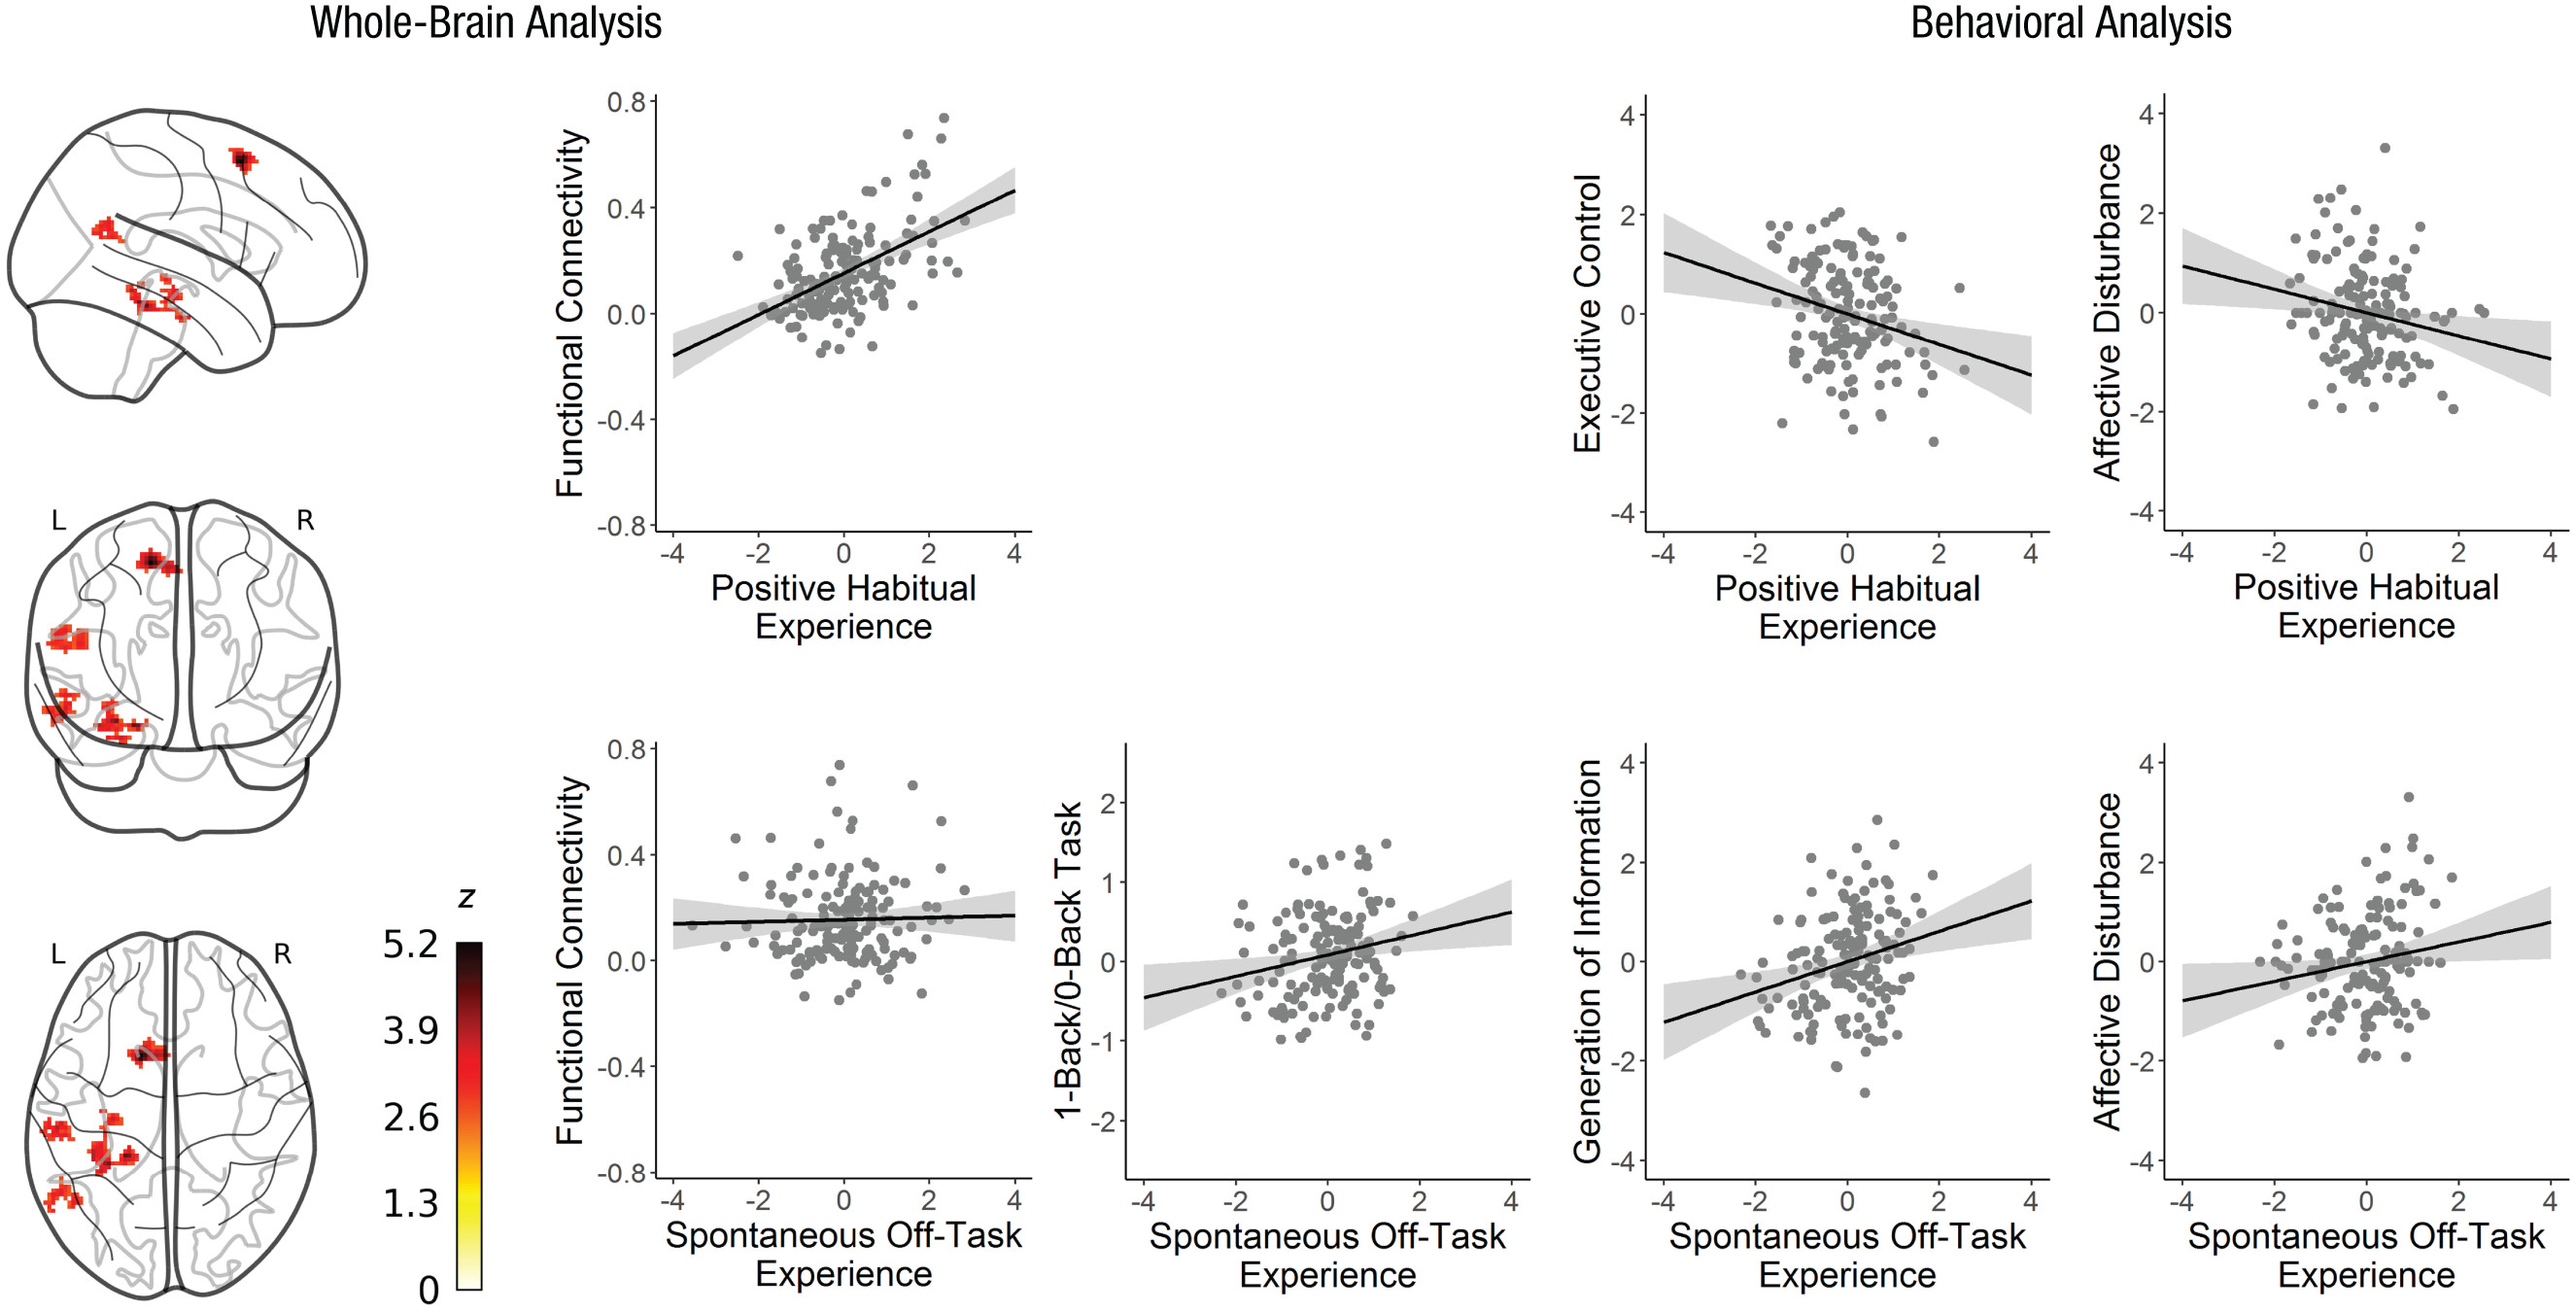
\includegraphics[width=0.8\textwidth]{chapters/img/study1fig4.jpeg}
	\caption{Relationship between the different neural-cognitive components and the laboratory and questionnaire measures.}
	\caption*{For the whole-brain analysis, the brain diagrams show clusters of the default-mode-network mask, and the graphs show the correlation between their functional connectivity and the two experience components. For the behavioral analysis, the graphs show the relationship between the two canonical components and measures of well-being and task performance.}

	\label{fig:study1:fig4}
\end{sidewaysfigure}

Next, we explored whether the different canonical components had specific implications for performance on the tasks in which we assessed experience (i.e., the 0-back/1-back task). Because the SCCA depends on resting-state data recorded independently of the task, we were unable to estimate the canonical components separately for each task. Consequently, in these analyses, we explored whether overall differences in canonical component loadings across participants were associated with performance efficiency on the 0-back/ 1-back task. We used a repeated measures analysis of variance in which the dependent variable was the efficiency with which participants performed the 0-back/ 1-back task, respectively. This analysis revealed a significant interaction between task efficiency and variation in our spontaneous-off task component, F(1, 154) = 6.43, p = .012, ηp2 = .04. Decomposition of this interaction showed that participants who scored higher on spontaneous off-task experience performed better on the 0-back condition, b = 0.06, 95\% confidence interval (CI) = [0.01, 0.11], t(151) = 2.38, p = .019, ηp2 = .04, and worse on the 1-back condition, b = −0.09, 95\% CI = [−0.15, −0.02], t(151) = −2.55, p = .012, ηp2 = .04. The differential relationship between the levels of spontaneous off-task experience and performance on the 0-back/1-back task is shown in Figure \ref{fig:study1:fig4}. These data confirm accounts that suggest that attentional lapses linked to mind wandering are context dependent, tending to have more negative effects as tasks become more demanding \cite{Smallwood2013a}; they are also consistent with prior studies suggesting that context regulation may be more problematic for spontaneous than deliberate mind wandering \cite<see also>{Seli2016}.

Finally, we used MANOVA to determine how the patterns of experience revealed by SCCA were related to the decompositions of the battery of cognitive performance and questionnaire measures. In this analysis, PCA scores describing either phenotypical variation or questionnaire measures on each of the components of cognitive function were the independent variables, and the individual loadings for each of the two canonical components describing experience from the SCCA were the dependent variables. For the analysis of phenotypical variation, this produced two significant results with the executive-control component, F(2, 152) = 5.84, p = .006, ηp2 = .065, and the generation-of-information component, F(2, 152) = 3.41, p = .007, ηp2 = .065. Higher loadings on the positive-habitual component, F(1, 153) = 9.84, p = .002, ηp2 = .060, were associated with worse performance on tasks requiring executive control, b = −0.19, 95\% CI = [−0.32, −0.07], t(153) = −3.14, p = .002, ηp2 = .060, and higher loadings on the spontaneous-off task experience component, F(1, 153) = 10.15, p = .002, ηp2 = .062, were associated with better performance on tasks involving the generation of information (such as creativity), b = 0.20, 95\% CI = [0.08, 0.33], t(153) = 3.19, p = .002, ηp2 = .062. This indicates that two of the experiential components identified by the SCCA were uniquely associated with poor performance on executively demanding tasks and better performance on measures of creativity: both aspects of psychological functioning that have previously been linked to mind wandering \cite<e.g.,>{Baird2012,McVay2009}. The relationships for both neurocognitive dimensions are shown in Figure \ref{fig:study1:fig4}.

In terms of the relationship to the questionnaire decomposition, we found a significant association with the first principal component, F(2, 151) = 3.76, p = .026, ηp2 = .05, which captured affective disturbance. This revealed two significant relationships: (a) a strong association with the positive-habitual component, F(1, 152) = 6.13, p = .014, ηp2 = .04, which suggests a negative association between positive-habitual thought and levels of affective disturbance, b = −0.16, 95\% CI = [−0.29, 0.03], t(152) = −2.48, p = .014, ηp2 = .04, and (b) an association with the spontaneous-off-task-experience component, F(1, 152) = 4.55, p = .035, ηp2 = .03, which suggests that higher loadings on this component were associated with higher levels of affective disturbance, b = 0.15, 95\% CI = [0.11, 0.28], t(152) = 2.13, p = .035, ηp2 = .03. This analysis demonstrates that the different canonical components have dissociable associations with respect to well-being, capturing aspects of the bidirectional relationship between the mind-wandering state and affective disturbance highlighted by prior research \cite<e.g.,>{Killingsworth2010,Ruby2013a}. Importantly, our analysis demonstrates that the different canonical components have dissociable associations with respect to well-being, which shows that our method captured both elements of the apparently contradictory analysis linking the mind-wandering state to well-being that has been highlighted by prior research.

One concern with resting-state functional connectivity arises from the possibility that the connectivity matrices are unduly affected by individual differences in motion \cite{Power2014}. Consistent with this possibility, our results showed a correlation at the group level between the positive-habitual component, r(155) = .363, p < .001, but not the spontaneous-offtask-experience component, r(155) = −.097, p = .229. Hence, we assessed the contribution of this association to our results linking positive-habitual thought to our measured phenotypes. We performed a series of stepwise analyses to identify the contribution that motion made to the phenotypical associations with positivehabitual thought. In these analyses, the canonical component was the dependent variable. We entered the principal components describing cognition or wellbeing in the first step and Jenkinson’s mean FD in the second step. Including motion significantly improved the predictive value of the model for well-being— Model 1: R2 = .06, F(4, 152) = 2.21, p = .07, ηp2 = .06; Model 2: R2 = .19, F(5, 151) = 6.95, p < .001, ηp2 = .19; model change: R2 = .13, F(1, 151) = 24.51, p < .001—as well as of the model for cognition: Model 1: R2 = .07, F(3, 153) = 3.92, p = .010, ηp2 = .07; Model 2: R2 = .18, F(4, 152) = 8.22, p < .001, ηp2 = .18; model change: R2 = .11, F(1, 152) = 19.65, p < .001. In the case of well-being, the explained variance of the affective disturbance component was not improved with the inclusion of motion—Model 1: affective-disturbance β = −0.20, t(152) = −2.48, p = .014, ηp2 = .04, 95\% CI = [−0.29, −0.03]; Model 2: affective-disturbance β = −0.20, t(151) = −2.59, p = .011, ηp2 = .05, 95\% CI = [−0.28, −0.03], Model 2: mean-FD β = 0.36, t(151) = 4.94, p < .001, ηp2 = .14, 95\% CI = [3.29, 7.67]. Thus, the relationship between affective disturbance and positive-habitual thought remained largely unchanged by the inclusion of motion as a nuisance variable. In the case of cognition, executive control accounted for less variance in the positive-habitual component when mean FD was included—Model 1: executive-control β = −0.24, t(153) = −3.14, p = .002, ηp2 = .06, 95\% CI = [−0.32, −0.07]; Model 2: executive-control β = −0.16, t(152) = −2.17, p = .032, ηp2 = .03, 95\% CI = [−0.25, −0.01]; Model 2: β = −0.34, mean-FD t(152) = 4.43, p < .001, ηp2 = .11, 95\% CI = [4.82, 12.56].

Unlike in the well-being analysis, motion explained a substantial amount of variance that was shared in the relationship between executive control and positive-habitual thought. To explore whether the positive-habitual component reflected an artefact of motion, we selected participants for whom movement greater than 0.2 mm occurred on less than 5\% of the resting-state data (N = 134) and reran the SCCA with the identical pipeline. This produced similar solutions for both positive-habitual and spontaneous off-task thought (see Fig. S4 in the Supplemental Material). Importantly, positive-habitual thought was not significantly correlated with motion, r(132) = .10, p = .236, but was correlated with poor executive control, r(155) = −.26, p = .001 (see Table S1 in the Supplemental Material for the full set of correlations). This final analysis shows that in a more restricted sample in which motion did not correlate with either latent component, we still observed a relationship between positive-habitual thought and poor executive control.

% ==========================================================================================================
\section{Discussion}
\label{study1:discussion}
Using multivariate pattern analysis, our study demonstrated that the content of the mind-wandering state is heterogeneous and confirmed hypotheses that different types of experience have differing functional associations \cite{Smallwood2013a}. Using a novel analysis strategy, we simultaneously decomposed self-reports of experience with descriptions of neural organization, revealing dimensions of experience with unique phenotypical associations: positive-habitual experiences and spontaneous off-task thoughts.
Poor executive control, a well-documented association of mind wandering \cite{McVay2009}, predicted variation in positive-habitual thoughts. This pattern of thinking was linked to coupling in the mPFC, a region important for assigning value to neural signals \cite{Roy2012}. It is possible that deficits in executive control during mind wandering emerge because of problems in assigning value to an external task, a view supported by evidence that financial motivation limits the impact of mind wandering on performance \cite{Mrazek2012}. We found that spontaneous off-task experiences simultaneously underlie the association between mind wandering and tasks of creativity \cite{Baird2012}, as well as problems in performing tasks requiring continuous monitoring of external information. Finally, while positive-habitual experiences are linked to improved well-being, spontaneous off-task experiences are associated with increased affective disturbance, which captures the apparent contradiction that mind wandering can be associated with both negative \cite<e.g.,>{Killingsworth2010} and positive \cite<e.g.,>{Poerio2016} emotional states. Together, these data provide the most convincing evidence to date that experience during mind wandering unfolds along a set of underlying dimensions and that these explain many of the phenotypical associations that have hitherto been associated with the mind-wandering state \cite{Smallwood2013a}.
Our study also demonstrates the complex contribution that the DMN makes to cognition. Strong DMN connectivity at rest was associated with an increased tendency for positive-habitual thoughts about the future, which corroborates previous research linking the DMN to mental time travel \cite{Karapanagiotidis2017,Schacter2007}. Participants also rated these experiences as habitual, a pattern that supports accounts of the role of the DMN in cognition as emphasizing automatic influences during mind wandering \cite{Christoff2016}. Spontaneous off-task thoughts, in contrast, showed weaker integration between core DMN regions and were linked to poor performance in the 1-back condition, a context in which task performance depends on the DMN functioning as a coherent network \cite{Konishi2015}. More generally, we found that states of high connectivity within the DMN (positive-habitual thoughts) were associated with more functional coupling to regions outside of the core network—a key prediction of the view that activity within the DMN reflects the integration of information from across the cortex \cite{Margulies2016}. It is important to note that our analysis shows that the behavior of the DMN at rest contains information about individual variation in the type of experiences that emerge during mind wandering. These data should not be taken as evidence that this system is exclusive in its role in mind wandering. Indeed, our whole-brain regression provides quantitative evidence that the interactions of the DMN with other regions, including those in the medial temporal lobe and the executive system (e.g., pre-SMA), are also important. In this way, our study supports recent theoretical perspectives \cite<e.g.,> {Christoff2016,Margulies2016}, as well as prior empirical results \cite<e.g.,>{Ellamil2016,Golchert2017,Smallwood2016} highlighting that regions other than the DMN core are important for mind wandering.
There are a number of limitations of the current analysis. First, our study focused on describing mind wandering as a trait. Prior work has shown similarities between state and trait measures of mind wandering in terms of (a) neural processing (e.g., trait: Smallwood et al., 2016; state: Christoff, Gordon, Smallwood, Smith, \& Schooler, 2009; Stawarczyk, Majerus, Maquet, \& D’Argembeau, 2011) and (b) psychological processes such as working capacity (e.g., trait: McVay \& Kane, 2009; state: Mrazek et al., 2012) and happiness (e.g., trait: Ruby et al., 2013; state: Killingsworth \& Gilbert, 2010). Nonetheless there are certain aspects of mind wandering that can be understood only by treating it as a state, such as its temporal features \cite{Christoff2016}. 
Second, our study measured mind wandering in the laboratory. Although there is a correspondence between mind wandering in laboratory and naturalistic settings \cite<e.g.,>{McVay2009a}, 
its form and content may depend on the contexts in which the experience emerges. Consequently, our findings should be supplemented by studies examining the occurrence of different types of experience in ecologically valid settings. Finally, our study did not find evidence for links with tasks that rely on semantic memory or for links to psychological traits other than well-being. This may have been due to our selection of neural regions or from our selection of questions. Prior studies have linked regions in the temporal lobe to the contents of thought \cite<e.g.,>{Smallwood2016}, 
a pattern of data that is consistent with a role of the semantic system in spontaneous thought \cite{Binder2009}. 
Other work has highlighted awareness of mind wandering as important in traits such as hyperactivity \cite{Franklin2017}. 
We anticipate that extending the selected regions of the cortex and the aspects of experience measured may extend our understanding of the mindwandering state to encompass forms of semantic processing and additional psychological traits.
In closing, our study provides the strongest evidence to date that the mind-wandering state is heterogeneous in its content, neural basis, and functional associations. We describe two neurocognitive dimensions capturing associations with attentional lapses, creativity and wellbeing, confirming much of the research on mind wandering conducted over the last decade. However, we also provide an explanation for why scientific accounts of mind wandering have been dominated by controversy, such as its relationship to happiness \cite{Killingsworth2010}, creativity \cite{Smeekens2016}, executive control \cite{McVay2009}, and the DMN \cite{Gilbert2007}. Our data suggest that these debates emerge from an erroneous assumption that mind wandering is a unitary psychological construct, when it is in fact made up of distinct states with unique neural correlates and functional associations. This ontological uncertainty has led to artificial controversies that hinder the development of a mature science of internal experience. Although our findings do not capture the full range of experiential dimensions on which the mind can wander, they convincingly demonstrate that it is untenable to characterize mind wandering as a uniform experience. As a discipline, we must embrace methodologies and analytical techniques that capture the complex nature of internal experiences, allowing researchers to accurately determine the contribution that they make to people’s lives.

% ==========================================================================================================
\chapter{Patterns of Thought: Population Variation in the Associations between Large-Scale Network Organisation and Self-Reported Experiences at Rest}
\chaptermark{Patterns of Thought}
\label{ch:study2}
%\setcounter{equation}{0}

\textit{The following chapter has been adapted from:\\}
Wang, H.-T., Bzdok, D., Margulies, D., Craddock, C., Milham, M., Jefferies, E., \& Smallwood, J.(2018). Patterns of thought: Population variation in the associations between large-scale network organisation and self-reported experiences at rest. \textit{NeuroImage}, Advance online publication. doi: 10.1016/j.neuroimage.2018.04.064
\footnote{
J. Smallwood, and H.-T. Wang designed the study. The data was provided from C. Cameron and M. Milham. The analysis pipeline was constructed by H.-T. Wang under the supervision of D. Bzdok and J. Smallwood. Data were analyzed by H.-T. Wang, under the supervision of D. Bzdok, J. Smallwood, and E. Jefferies. H.-T. Wang and J. Smallwood drafted the manuscript. D. Bzdok, D. Margulies and E. Jefferies provided critical input to the interpretations. All the authors approved the final version of the manuscript prior to submission.}
\\

%Abstract
\newpage
\noindent{}Contemporary cognitive neuroscience recognises unconstrained processing varies across individuals, describing variation in meaningful attributes, such as intelligence. It may also have links to patterns of on-going experience. This study examined whether dimensions of population variation in different modes of unconstrained processing can be described by the associations between patterns of neural activity and self-reports of experience during the same period. We selected 258 individuals from a publicly available data set who had measures of resting-state functional magnetic resonance imaging, and self-reports of experience during the scan. We used machine learning to determine patterns of association between the neural and self-reported data, finding variation along four dimensions. "Purposeful" experiences were associated with lower connectivity - in particular default mode and limbic networks were less correlated with attention and sensorimotor networks. "Emotional" experiences were associated with higher connectivity, especially between limbic and ventral attention networks. Experiences focused on themes of "personal importance" were associated with reduced functional connectivity within attention and control systems. Finally, visual experiences were associated with stronger connectivity between visual and other networks, in particular the limbic system. Some of these patterns had contrasting links with cognitive function as assessed in a separate laboratory session - purposeful thinking was linked to greater intelligence and better abstract reasoning, while a focus on personal importance had the opposite relationship. Together these findings are consistent with an emerging literature on unconstrained states and also underlines that these states are heterogeneous, with distinct modes of population variation reflecting the interplay of different large-scale networks.

% ====================================================================================================================
\section{Introduction}
\label{study2:intro}
Unconstrained processing reflects important population level variation in measures of cognition, affect, and demographic \/ lifestyle factors. Psychological studies show that almost a third of on-going thought is unconstrained by events in the here-and-now \cite{Killingsworth2010} with important links to cognitive and affective processing \cite{Mooneyham2013}. In neuroscience, metrics defined from the brain during wakeful rest, describe the organisation of neural function at both the micro and macro scale \cite{Glasser2016,Margulies2016}. They also reflect individual differences in cognitive function \cite{Finn2015}, psychiatric conditions \cite{Nooner2012} and demographic \/ lifestyle factors \cite{Smith2015}. These findings establish unconstrained neurocognitive processing as a core element of human cognition, highlighting the need to formally understand the underlying neural architecture, and the associated patterns of experience.

One perspective on unconstrained processing emphasises the role of memory, with contributions of conceptual and episodic representations to ongoing thought \cite{Binder2009,Gusnard2001}. 
Psychological studies have shown patterns of unconstrained processing have links with memory retrieval, creativity and planning \cite{Baird2012,Leszczynski2017,Medea2016,Poerio2017}. 
Such evidence raises the possibility that episodic representations anchored in the medial temporal lobe \cite{Moscovitch2016} 
or conceptual representation anchored in anterior temporal lobe \cite{Lambon-Ralph2016} 
contribute to on-going thought \cite{Smallwood2016}. 
It is hypothesised that these systems contribution to unconstrained states may be linked to the ability for these regions to become functionally decoupled from systems more directly involved in action and perception, allowing them to operate in an offline manner \cite{Smallwood2013a}. 
This process of decoupling may also be important in neural systems closely allied to those involved in memory – the default mode network \cite{Raichle2001}. 
These regions of transmodal cortex are relatively distant in functional and structural space from systems involved in perception and action, potentially facilitating their role in stimulus independent aspects of cognition \cite{Buckner2013,Margulies2016,Mesulam1998}. 
Together these "representational" accounts of unconstrained processing highlight default mode and limbic networks as important candidate neural systems, especially when decoupled from systems directly involved in perception and action.

Alternative perspectives on unconstrained thought emerge from links between types of ongoing experience and problems maintaining a task relevant goal in mind. This “executive-failure” view \cite{Kane2012,McVay2009}%(Kane \& McVay, 2012; McVay \& Kane, 2010) 
takes as a starting point evidence that patterns of on-going thought, such as the experience of mind-wandering, are linked to problems on tasks including sustained attention \cite{McVay2009}
and measures of general aptitude and executive control \cite{Mrazek2012}. 
Task-based neuroimaging investigations highlight a network of regions that increase their activity across many different task situations, so called multiple demand regions \cite{Duncan2010}. %(Duncan, 2010). 
These regions broadly correspond to three well described intrinsic networks: ventral attention, dorsal attention, and frontal-parietal networks. Since these systems are important for the effective performance of many different tasks then dysregulation within these systems could reflect the hypothesised "executive-failure" contribution to aspects of ongoing thought \cite{McVay2009,Weissman2006}.%(McVay \& Kane, 2010; Weissman, Roberts, Visscher, \& Woldorff, 2006).

Other aspects of unconstrained processing could reflect the importance of affective processes, or different modalities of processing. Ongoing thought is linked to mood state: Experimental inductions of mood \cite{Smallwood2009a,Smallwood2011}
%(Smallwood, Fitzgerald, Miles, \& Phillips, 2009; Smallwood \& O'Connor, 2011)
as well as natural fluctuations \cite{Poerio2013, Ruby2013a}
%(Poerio, Totterdell, \& Miles, 2013; Ruby, Smallwood, Engen, \& Singer, 2013) 
impact on ongoing thought. Contemporary accounts of emotional processing emphasise the role of limbic regions including the amygdala \cite{Bzdok2013,Lindquist2012}%(Bzdok, Laird, Zilles, Fox, \& Eickhoff, 2013; Lindquist, Wager, Kober, Bliss-Moreau, \& Barrett, 2012) 
and anterior aspects the insula \cite{Touroutoglou2012},%(Touroutoglou, Hollenbeck, Dickerson, \& Barrett, 2012), 
suggesting these regions may be important in determining affective aspects ofongoing thought. Psychological studies of ongoing thought also suggest that another important dimension of unconstrained processing may reflect the different modalities of processing \cite{Konishi2017,Smallwood2016}%(Konishi, Brown, Battaglini, \& Smallwood, 2017; Smallwood et al., 2016). 
It has been shown, for example, that the visual system plays an important role in the expression of visual imagery \cite{Ganis2004,Kosslyn2001}.%(Ganis, Thompson, \& Kosslyn, 2004; Kosslyn, Ganis, \& Thompson, 2001). 
Recent work has extended this evidence to shown patterns of activity with visual regions are linked to the emergence of visual, non-verbal, elements of ongoing thought \cite{Raij2017}%(Raij \& Riekki, 2017). 
It is also possible that sensorimotor processes may be implicated in language processing during unconstrained processing, given that a role for these regions in langauge processing extends beyond production \cite{Bzdok2016,Pulvermueller2010,Pulvermueller2010a}.
%(Bzdok et al., 2016; Pulvermuller, 2010; Pulvermuller \& Fadiga, 2010).

Our study aimed to identify patterns of intrinsic connectivity associated with different patterns of unconstrained states and examines their neurocognitive features from the perspectives outlined above. We used a large publicly available dataset, containing measures of resting-state functional magnetic resonance imaging (fMRI), and an accompanying self-report instrument describing cognition experienced during the resting state \cite{Gorgolewski2014,Nooner2012}. We previously explored the relationships between patterns of on-going thought and measures of neural activity, such as the fractional amplitude of low frequency oscillations, as well as the regional homogeneity of neural activity, in a sub sample of this data set \cite{Gorgolewski2014}. In this study we focused on connectivity, we applied sparse canonical correlation analysis (SCCA) to obtain a conjoined decomposition of self-reports of experience with matrices of whole brain connectivity data. This analysis produces multivariate patterns that reflect dimensions of variation that are mutually constrained by both brain and experience. In this way we capitalize on the fact that self-reports of experience during scanning and descriptions of on-going neural processing provide complementary descriptions of unconstrained cognition. Our analysis, therefore, helps define, at a population level, the shared links between brain patterns and different types of experience. Moreover, respecting the multivariate nature of brain and behaviour space, as our analysis does, can accommodate complex many-to-many relationships between patterns of connectivity and self-reports, and therefore is sensitive to the possibility of degeneracy in the underlying data. As a final validation step we established whether these neurocognitive dimensions are associated with performance on a battery of available cognitive tasks, including measures of executive control and intelligence.

We use the dimensions our analysis produces, and their links with cognitive function to evaluate the perspectives on unconstrained thought outlined earlier. "Representational" accounts emphasise links with neural systems involved in memory, such as the limbic system, and regions of transmodal cortex, such as the default mode network. They highlight states with lower levels of functional communication between these regions and those more directly involved in external action. In contrast, "executive-failure" accounts emphasise dysregulation in attention and control networks as contributing to patterns of ongoing thought that are linked to problems in domain general task performance. Affective accounts highlight limbic regions as important hubs in aspects of ongoing thoughts linked to emotion. Finally, modality specific influences on unconstrained thought may depend on information codes represented in regions that specialise in that particular types of information, such as a role of visual cortex in experiences dominated by images. Notably, some views lead to dissociable predictions with respect to cognitive performance. For example, executive-failure accounts predict patterns of thoughts linked to worse performance on measures of cognitive function, while representational accounts makes the alternative prediction.
% ==========================================================================================================

\section{Method}
\label{study2:method}

\subsection{Participants}
\label{study2:method:participants}
We analysed 258 participants (females = 162; age range 18 – 55, M = 34.97, SD = 12.24) obtained from the enhanced Nathan Kline Institute-Rockland sample (NKI-RS; \url{http://fcon_1000.projects.nitrc.org/indi/enhanced/}).
Full details of the acquisition of this sample can be found in Nooner et al., 2012. 
We selected participants between 18 and 55 years old as our sample, this choice allowed us to maximise the cohesive nature of our sample.  All the participants have the MRI data and less than 5 missing data points among the selected assessments.

\subsection{Cognitive measures and questionnaires}
\label{study2:method:cog}
Based on prior studies examining the links between spontaneous thought and cognitive performance \cite<see>{Mooneyham2013}, %(see Mooneyham \& Schooler, 2013) 
we selected established neuropsychological measures linked to executive control, abstract reasoning and intelligence. The measures included the Delis-Kaplan Executive Function System \cite<D-KEFS;>{Swanson2005},
Wechsler Abbreviated Scale of Intelligence \cite<WASI-II;>{Wechsler1999}, 
and Wechsler Individual Achievement Test – Second Edition Abbreviated \cite<WIAT-IIA;>{Wechsler2005}.  
In D-KEFS we selected the tower test (move accuracy ratio), colour-word interference test (errors inhibition/switching), verbal fluency test (letter fluency - category fluency), design fluency test (design accuracy), trail making test (sequencing errors score + set-loss errors score + time-discontinue errors score), and the proverb test (a measure of abstract semantic reasoning). We used the rescaled score (M = 10, SD = 3) in our analysis. Tasks measures that reflected error rates (i.e. the colour-word interference test and trail making test) were reversed, so that high rescaled scores indicated better task performance. All the scores were transformed to z-scores.

\subsection{On-going cognition measure}
\label{study2:method:NYCQ}
The New York Cognition Questionnaire (NYC-Q) is a self-report tool used to assess the thoughts experienced at rest \cite{Gorgolewski2014,Sanders2017}.%(Gorgolewski et al., 2014; Sanders, Wang, Schooler, \& Smallwood, 2017). 
It assesses thoughts and feelings experienced during the resting-state period. The first section contains 23 questions about the content of thought. These questions covers the temporal, social, emotional aspects of spontaneous thoughts that have been shown to be important by prior studies \cite<e.g.>{Ruby2013a}. 
Participants rated each question on a scale of 1 (Completely did not describe my thoughts) to 9 (Completely did describe my thoughts). The second section contains 8 questions about the forms thoughts take, capturing aspects of experience such as modality and detail associated with experience that prior studies suggest as important for spontaneous thoughts \cite{Smallwood2016}. 
Participants rated each question on a scale of 1 (Completely did not characterise my experience) to 9 (Completely did characterise my experience).  In the current study we analysed the two sections together to provide single solutions that combined information on both the content form of experience. The full list of questions and the corresponding labels are presented in Table \ref{tab:study2:1}. The questionnaire was administrated once after the resting-state scan in order to assess experiences during the scanning session. For the full details of the NYC-Q, please refer to \citeA{Gorgolewski2014}. 
We have placed the questionnaire measure used in this study along with an example self-report collection task on GitHub at the following address:
\url{https://github.com/htwangtw/restingstate_thoughtreports}.

\linespacesmall

\begin{table}
\centering
\caption{The New York Cognition Questionnaire (NYC-Q).}
\label{tab:study2:1}

\resizebox{\textwidth}{!}{
\begin{tabular}{ l l}
\toprule
Questions&Labels\\ 
\midrule
I thought about things I am currently worried about&Concerns\\
I thought about people I have just recently met&People\\
I thought of people I have known for a long time (friends)&Friend\\
I thought about members of my family&Family\\
I thought about an event that took place earlier today&Today - Past\\
I thought about an interaction I may possibly have in the future&Social - Future\\
I thought about an interaction with somebody that took place in the past&Social - Past\\
I thought about something that happened at a place very close to me&Near Location\\
I thought about something that made me feel guilty&Guilt\\
I thought about an event that may take place later today&Today - Plan\\
I thought about something that happened in the recent past (last couple of days but not today)&Recent Past\\
I thought about something that happened a long time ago in the past&Distant Past\\
I thought about something that made me angry&Anger\\
I thought about something that made me happy&Happiness\\
I thought about something that made me cheerful&Cheerfulness\\
I thought about something that made me calm&Calm\\
I thought about something that made me sad&Sadness\\
I thought about something that is important to me&Importance\\
I thought about something that could still happen today&Today - Future\\
I thought about something that may take place in the distant future&Distant Future\\
I thought about something that could take place in the near future (days or weeks but not today)&Near Future\\
I thought about personal worries&Worries\\
I thought about something that happened in a place far away from where I am now&Distant Location\\
In the form of images:&Image\\
In the form of words:&Words\\
Like an inner monologue or audiobook:&Monologue\\
Like a television program or film:&Film\\
Had a strong and consistent personal narrative:&Narrative\\
Had a clear sense of purpose:&Purpose\\
Vague and non-specific:&Vague\\
Fragmented and disjointed:&Fragment\\
\bottomrule
\end{tabular}
}
\end{table}

\linespacenormal
\subsection{MR data processing}
\label{study2:method:MRI}

\subsubsection{Resting-state fMRI} 
We used resting-state fMRI to describe the general functional organisation of the brain. We selected resting-state multiband functional magnetic resonance imaging (R-mfMRI;  TR = 1400msec; voxel size = 2mm isotropic; duration = 10 minutes) for our analysis. Functional and structural data were pre-processed using Configurable Pipeline for the Analysis of Connectomes (C-PAC; \url{https://fcp-indi.github.io/}) to interface with FMRIB’s Software Library (FSL version 5.0, \url{www.fmrib.ox.ac.uk/fsl}). Individual FLAIR and T1 weighted structural brain images were extracted using Brain Extraction Tool (BET). Structural images were linearly registered to the MNI-152 template using FMRIB's Linear Image Registration Tool (FLIRT). The resting-state functional data were pre-processed and analysed using the FMRI Expert Analysis Tool (FEAT). X, Y, Z displacement and the three axis rotations were used to calculate the mean frame displacement (FD), characterising movement of each participant during the scanning session (Power et al., 2014). Mean of the absolute values for FD were later used to account for subject specific head motion. No global signal regression was applied. The individual subject analysis involved: motion correction using MCFLIRT; slice-timing correction using Fourier space time series phase-shifting; spatial smoothing using a Gaussian kernel of FWHM 6 mm; bandpass filtering (0.1 Hz $<$ f $<$ 0.009 Hz); six motion parameters (as estimated by MCFLIRT) regressed out; cerebrospinal fluid and white matter signal regressed out (top five PCA components, CompCor method). 

\subsubsection{Connectivity matrices} 

To describe the functional architecture of the whole brain, we transformed the resting-state BOLD time series into connection strength values of the different networks for each participant. The whole brain parcellation was obtained from connectivity-based functional parcellation created by Yeo and collegues \citeyear{Yeo2011}. 
The 7 network parcellation was used in the current study. We split the networks into two hemispheres and extracted clusters. Two voxels are considered connected only if they are adjacent within the same x, y, or z direction. This yielded 57 clusters from the Yeo 7 networks parcellation. The implementation of spatial clusters extraction was retrieved from python library Nilearn \cite[\url{http://nilearn.github.io/}, version 0.3.1]{Abraham2014}
Next, we extracted and then averaged the time series of all voxels within each cluster to create a cluster specific time series. We used these time series to create region-to-region symmetrical correlation matrices representing the correlations of the network signal that was computed for all the individual subjects. The off-diagonal of each correlation matrix contained 1596 unique region-region connection strengths (i.e., the upper or lower triangle of the network covariance matrix). This approach provided a measure of connection strength of the whole brain for each participant. Finally, Fisher’s r-to-z transformation was applied to each network covariance matrix.

\subsection{Conjoint decomposition of connectivity and experience}
\label{study2:method:ML}

\subsubsection{Decomposition methods}
\label{study2:method:ML:CCA}
We performed a sparse canonical correlation analysis \cite<SCCA; see>{Hastie2015}%{ Hastie, Tibshirani, \& Wainwright, 2015} 
on the functional connectomes and the NYC-Q reports, to yield latent components that reflect multivariate patterns across neural organisation and experience \cite<For similar application, see>{Wang2018}%Wang et al., 2017). 
SCCA maximised the linear correlation between the low-rank projections of two sets of multivatiate data sets with sparse model to regularise the decomposition solutions a process that helps maximise the interpretability of the results. The regularisation function of choice is L1 penalty, which produces ‘sparse’ coefficients, meaning that the canonical vectors (i.e., translating from full variables to a data matrix’s low-rank components of variation) will contain a number of exactly zero elements. L1 regularisation conducted (i) feature selection (i.e., select only relevant components) and (ii) model estimation (i.e., determine what combination of components best disentangles the neuro-cognitive relationship) in an identical process. This way we handle adverse behaviours of classical linear models in high-dimensional data. A reliable and robust open-source implementation of the SCCA method was retrieved as R package from CRAN 
\cite<PMA, penalized multivariate analysis, version 1.0.9>{Witten2009a}%(PMA, penalized multivariate analysis, version 1.0.9, Witten, Tibshirani, \& Hastie, 2009).
The amount of L1 penalty for the functional connectomes and the NYC-Q reports were chosen by cross-validation. The procedure is described below. 

\subsubsection{Model selection}
\label{study2:method:ML:model}
We employed cross-validation (CV) to select the most useful model across population samples and avoid overfitting \cite{BzdokYeo2017}.
The amount of the two L1 penalty terms for the functional connectomes and the NYC-Q reports, respectively, were chosen by a nested K-fold CV, where the coefficient for the penalty were chosen using a grid search to maximise the quality of CV objective metric. The objective metric of choice cumulative explained variances. The explained variance of each latent component was calculated using the squared canonical correlation. High explained variance suggests a high pattern recovery rate between the two data set. The sparse assumption is fundamentally in conflict with the statistical goal of finding components with high explained variance. Therefore we decided the number of components in the model before searching for the best parameter. 

We performed confound removal on functional connectomes and the NYC-Q reports as suggested by prior studies \cite{Smith2015}. 
We removed the effects of nuisance variables from the dataset. These confound variables were sex, age, and head motion indicated by Jenkinson’s mean FD \cite{Jenkinson2002}.%Jenkinson, Bannister, Brady, \& Smith, 2002). 
The removal steps was performed on the training set in each CV fold. We standardized the confound by calculating the z-score, and also squared the three confound measures to account for potentially nonlinear effects of these confounds. The 6 resulting confounds were regressed out of both data matrices. The implementation of the confound removal method \cite{Friston1994} 
was retrieved from python library Nilearn \cite[\url{http://nilearn.github.io/}, version 0.3.1]{Abraham2014}.

The number of latent components was determined by a preliminary analysis with no sparsity and calculated the explained variances for the two datasets (i.e., brain network correlations and questionnaire ratings). The explained variance increased with the number of components and growth stabilised at 10 components. We selected the number of components based on the point where the tangent stabilised. This led to a model of  4 components, and it accounted for a total of 78\% of the variance in connection strength and 29\% of the variance in the self-report data. Next, we determined the two coefficients for the L1 penalty terms that was associated with the best model performance with 4 latent components. We searched for the best L1 penalty values between 0.1 and 0.9 in 0.1 increments, which resulted in 81 set of parameters. For the nested K-Fold CV, we first separate the data into 5 consecutive folds after shuffling the data and retained one fold as the evaluation set (N ~= 50); the other four folds were used as the development set. The development set was further separated into 5 folds for parameter selection and each fold (N ~=40) was used as the validation set once. The model was estimated on the training folds with all parameter sets, and after completion, we trained the model with the winning parameter on the whole development set and the finally tested the performance on the independent, unseen evaluation set. We selected the final parameters according to the best performance on the evaluation set across all folds of the outer CV loop (Figure 1). This parameter set is used to train on the full development set and tested on the evaluation set. The parameter grid search and k-fold CV was conducted by the implementation in a Python library scikit-learn \cite<http://scikit-learn.org/stable/, version 0.18.2>{scikit-learn}.
The detailed algorithm for selecting the penalty values are presented in  Appendix \ref{appendix:kfold}: Nested K-Fold CV.

\begin{figure}
	\centering
	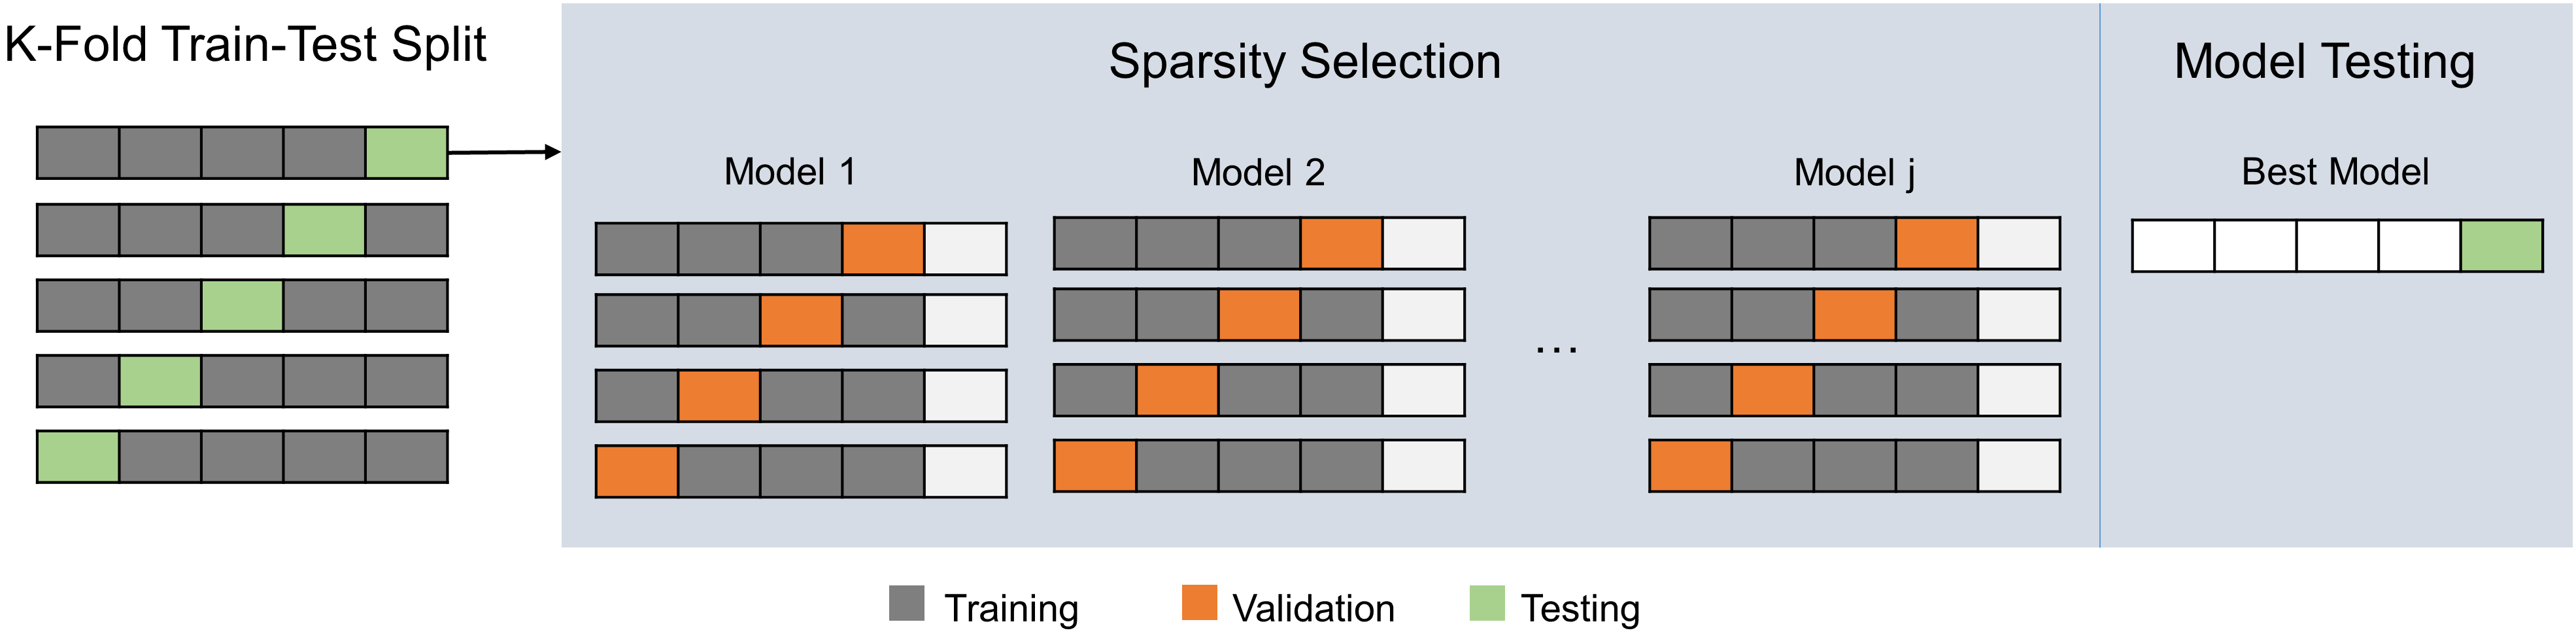
\includegraphics[width=0.8\textwidth]{chapters/img/study2fig1.png}
	\caption{A diagram of the nested k-fold cross-validation with model selection.} 
	\caption*{
	\footnotesize{
	The model with the best test performance was selected as the final model. The final model’s sparsity coefficient are 0.8 (functional connectivity) and 0.5 (self-reports), and the out-of-sample explained variance was 48\%. We used the ensuing canonical vectors of the winning SCCA model to compute the latent component scores. There are two sets of canonical scores in a latent component, a weighted sum of variables forms the canonical vectors. For each latent component, we averaged the z-score of the canonical scores of the connection strength and NYC-Q as the combined scores. These scores described the summary of the experience with both the neural basis and the content reports.}
	}
	\label{fig:study2:fig1}
\end{figure}

\subsection{Test of component robustness}
\label{study2:method:robust}
After identifying the well performed components in compressing the brain-experience data, we examined the robustness of the four components in two different ways. The permutation test is a purely data-driven strategy that access the chance of discovering components in null samples. We also leveraged the brain-experience components to explain the cognitive functions, so that we can identify meaningful patterns by well-established cognitive measurements. 

\subsubsection{Permutation test}
\label{study2:method:permute}
We used permutation testing to assess the robustness of the components identified through our analysis. We constructed a null distribution for each canonical component by holding the functional connectivity data in place and randomising the row order of self-reports data. This permutation scheme broke the link of individual differences in the dataset, therefore testing the robustness of the components in the hypothetical population. By calculating the false-discovery rate in the null distribution, we can conclude the possibility of discovering our components by chance with the given penalty coefficients. Hypotheses that are accepted with a 5\% level of significance. In the current analyses we adopt the permutation test with the FWE-corrected p-value by Smith and colleagues \citeyear{Smith2015}.
with data argumentation to increase the size of the resampling datasets to 1000. The four components were compared to the first sparse canonical correlation of the permuted sample. The low-rank components are more relevant that the rest, therefore we yield more conservative p-value by comparing to the first canonical correlation only. We performed 5000 permutation tests to get enough estimates for 4 decimal places. 

\subsubsection{Group analysis}
\label{study2:method:manova}
To determine how patterns of unconstrained neuro-cognitive activity related to performance on the battery of cognitive tests, we conducted an independent statistical analysis on the identical subjects. A Type III multivariate multiple regression with Pillai’s trace test was applied to 4 individual scores for each of the latent components describing experience from the SCCA  were the independent variables, and the original 8 measures of cognitive performance were the dependent variables that we hoped to described by the linear combination of the latent components. Pillai’s trace test is considered to be the most powerful and robust statistic for general use \cite{Huberty2006}.%(Huberty \& Olejnik, 2006). 
The p-values reported were based on Bonferroni correction. We also performed a principal components analysis (PCA) to identify the patterns of covariance among the 8 measures of cognitive performance and compressed the data. The relation between the principle score and the 4 brain-expereince diemsnons identified through SCCA was examined in a linear regression model with Pillai’s trace test. The analysis was conducted in R (version 3.3.1).  The multivariate multiple regression was conducted in R (version 3.3.1) using function ‘Manova’ in R package ‘car’ (companion to applied regression, version 2.1-5). 

\subsection{Code availability}
\label{study2:method:code}
The full analysis pipeline is freely available at \url{https://github.com/htwangtw/patterns-of-thought}. 

% ==========================================================================================================

\section{Results}
\label{study2:results}

\subsection{Determining constituent category of experience}
\label{study2:results:cca}
We used Sparse Canonical Correlation Analysis (SCCA) to determine connectome-wide dimensions that describe common variance shared by descriptions of brain and experience. This took as input individual scores for the connections between each of the regions extracted from Yeo’s 7 networks parcellation and the scores of each item of the New York Cognition Questionnaire (NYC-Q).

We applied SCCA with nested 5-fold CV as the model selection strategy. We obtained a model of 4 canonical components with penalty levels of 0.8 on the functional connectivity and 0.5 on the NYC-Q that indicated the best out-of-sample prediction on our data (see 3.5.2 Model Selection). The canonical correlations of the 4 latent components were 0.28, 0.19, 0.16, and 0.07. The latent components yielded by the best model are presented in Figure 2. For the ease of presentation and interpretation, we summarized the components as network-network connectivity instead of 57-by-57 connectivity matrices. The heat maps describe the network-to-network correlations while the word clouds describe the loadings on the self-report items. The components in full and the heat map for the self-report items can be found in Online Supplementary Materials.

\begin{figure}
    \centering
    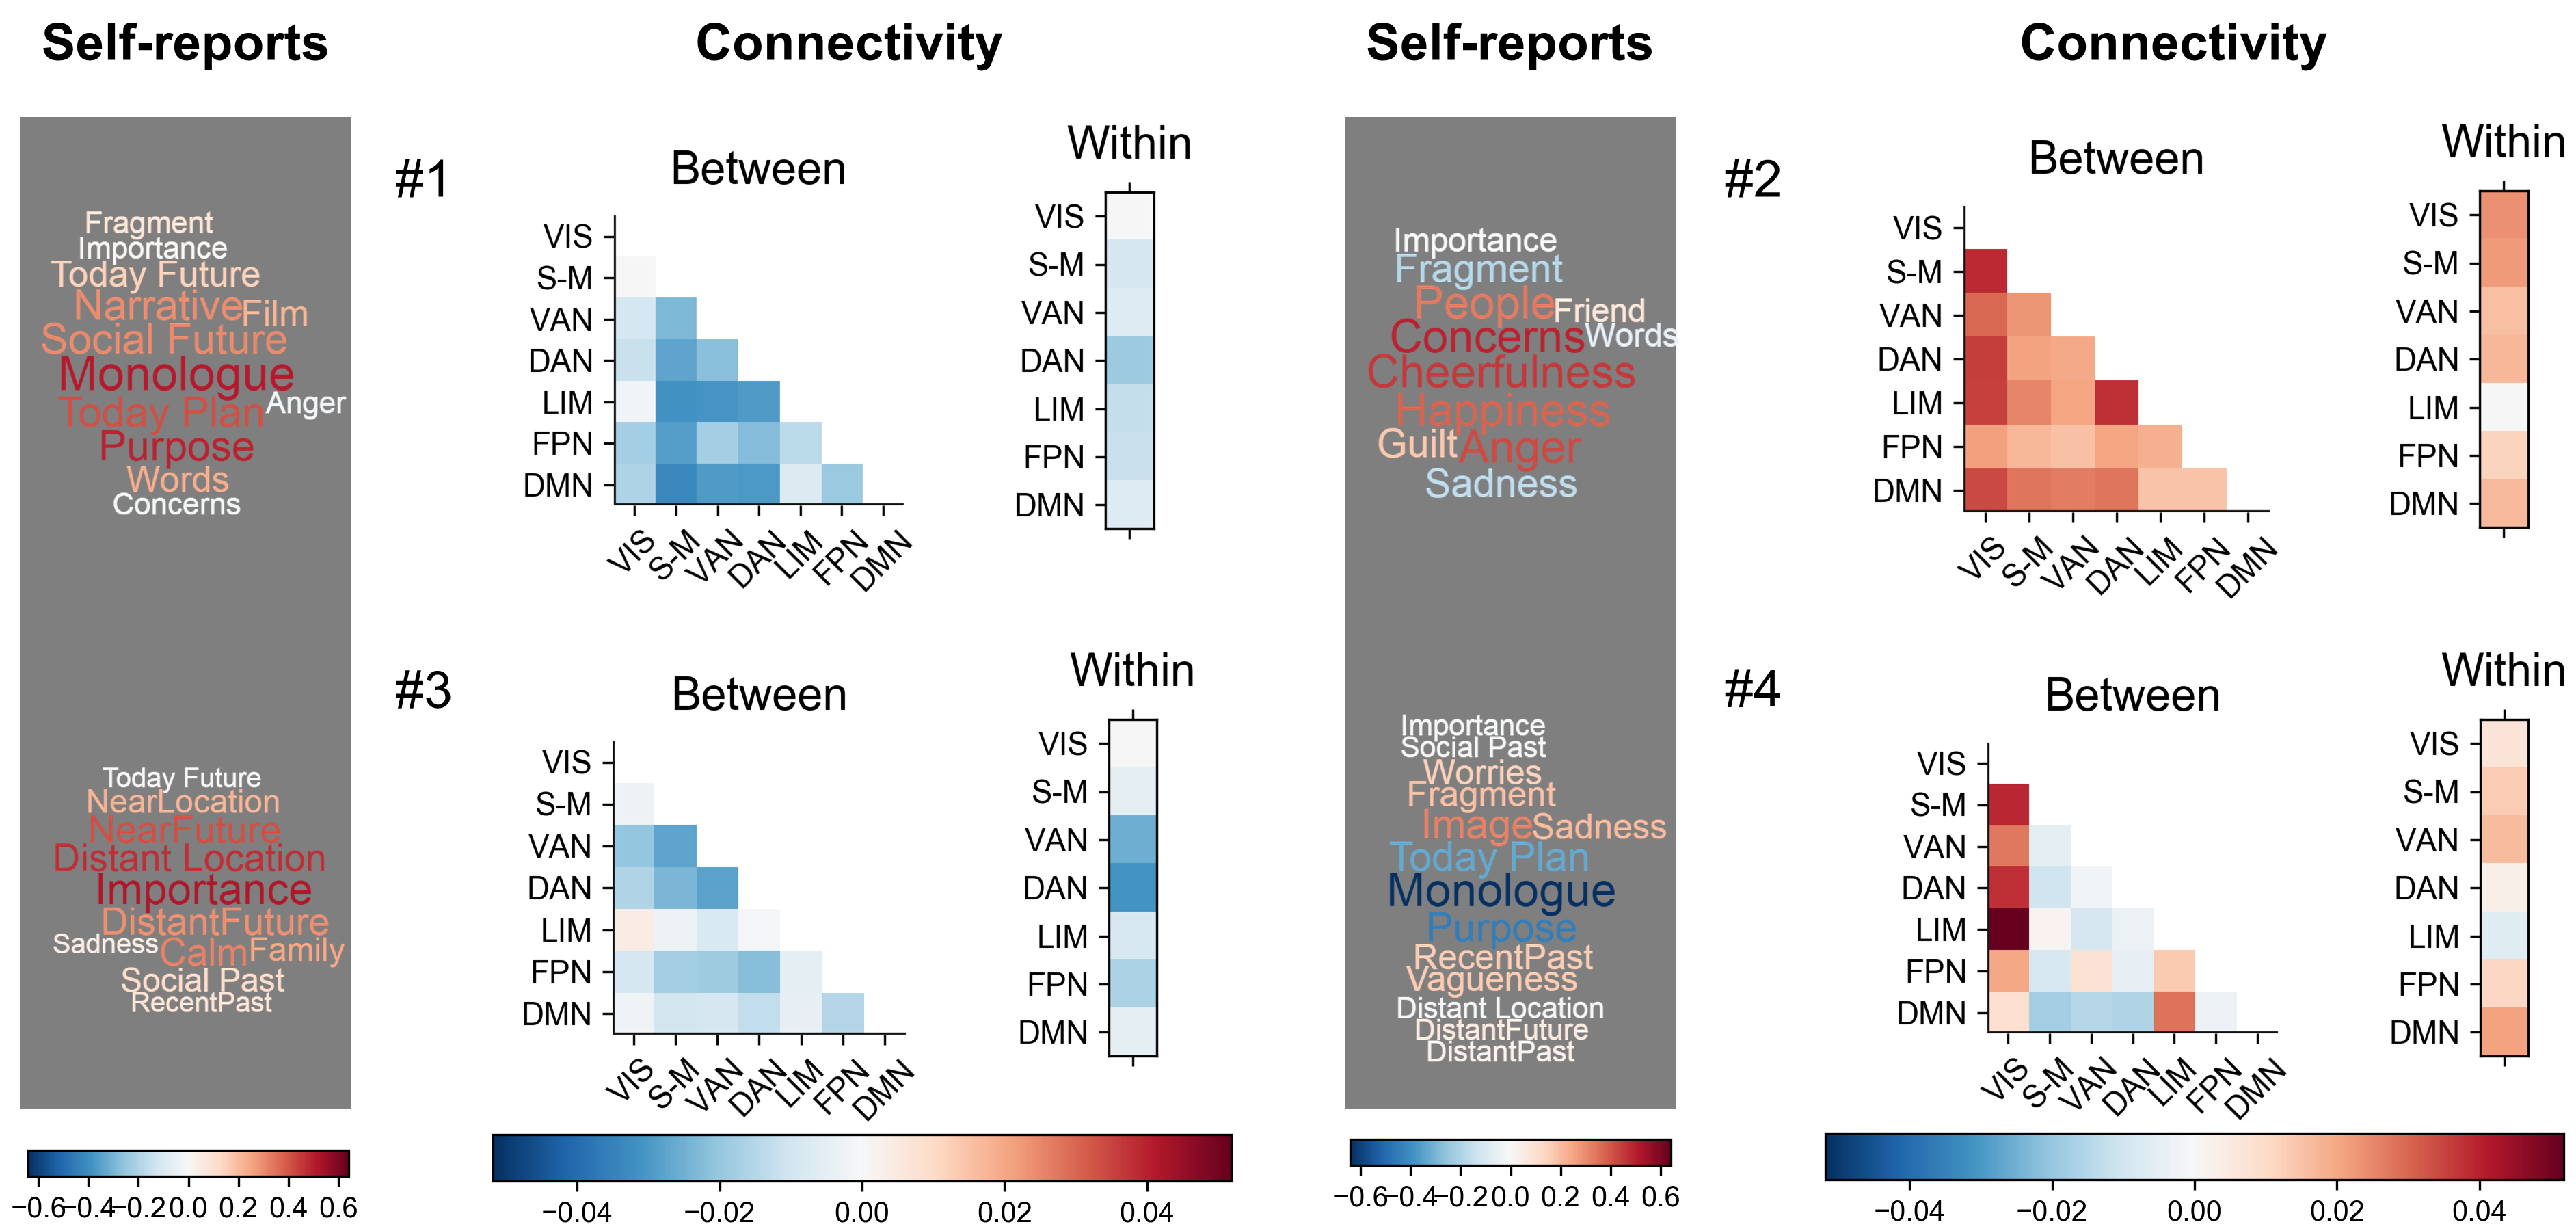
\includegraphics[width=0.8\textwidth]{chapters/img/study2fig2.png}
    \caption{Unique neuro-cognitive dimensions of population variation revealed by sparse canonical correlation analysis of measures of whole brain connectivity and self-reported descriptions of on-going experience.} 
    \caption*{
    \footnotesize{
    The heat map describes the canonical variate of the network-to-network connectivity between different Yeo networks. The connectivity matrices describes the coefficients from the model, separated into within and between network relationships. The word clouds reflect the coefficients on the relevant self-report items. In both cases the colour bars indicate the magnitudes of the coefficients. A detailed version of the canonical variates and alternative presentation of the self-report coefficients can be found in Supplementary Material Figure S1- S5.}
    }
    \label{fig:study2:fig2}
\end{figure}

Component 1, describes patterns of reduced within network connectivity within all of the networks studied, with this pattern most prominent in the dorsal attention network. Between network connections are generally reduced, with the exception of visual to limbic. Sensorimotor was decoupled from all the other systems, and, in addition, the default and limbic were most decoupled from the attention networks. Experiential themes in Component 1 are dominated by themes related to deliberate planning with a verbal component (high loadings on “words”, “monologue”, “today-plan”, “social-future”, “purpose” and “deliberate”). We refer to this pattern of reports as reflecting thoughts with “purpose”. 

Component 2 is dominated by relatively higher within and between network connections. Connectivity within each network was strong with the exception of the limbic network. Between network connections were stronger, with this pattern most apparent in the connections between limbic and ventral attention. In addition, the visual network was strongly correlated with the other networks. This component is dominated by emotional responses (high loadings on “anger”, “guilt”, “cheerfulness” and “happiness”) and social content (“friends” and “people”). We refer to this pattern of reports as reflecting “emotional” experience.

Component 3 emphasises reduced connections both between and within networks. Within network connectivity is weakest for the dorsal and ventral attention networks. Edge-to-edge connections are low, with the ventral and dorsal attention and fronto-parietal networks showing reduced correlations with each other as well as the visual and sensorimotor systems. This component was characterised by themes linked to personal “importance” with social temporal contents (“distant future”, “near future”, “social past”, “family” and “recent past”). We refer to this pattern of reports as reflecting “personal importance”.

Component 4 has the most heterogeneous pattern of within and between network connectivity. It is associated with stronger connections within networks with the exception of the limbic system. In addition, the visual system was strongly connected to all other networks, with this pattern most apparent for the limbic network. In contrast, lower network-to-network connectivity was observed between the default mode and sensori-motor and attention networks. This component is characterised by experiential patterns reflecting a modality difference in experience, with the highest loadings on “images” and lowest on “inner monologue”. We refer to this pattern of reports as describing “modality”. 


\subsection{The relationship between neuro-experiential components and cognitive functions}
\label{study2:results:manova}
Having documented four neuro-cognitive dimensions, we next examined the robustness of the components using two complementary approaches. We first used a permutation test to identify the chance of discovering components in a null samples as employed by Smith and colleagues (2015). The top three components passed the permutation test and the 4th component showed variance that was similar to that produced in a null sample (Component 1 p = 0.0002; Component 2 p = 0.0010; Component 3 p = 0.0204, Component 4 p = 0.998, α = 0.05). This analysis suggests that Components 1 – 3 are unlikely to have occurred by chance. Component 4 may be a Type II error and so we discuss this component in only a limited manner moving forward.
Our next test of the robustness of our components is whether they explained unique patterns of expertise in our battery of cognitive tasks. We used multiple multivariate regression model in which performance on the battery of selected tasks was the dependent variables and the individual scores for each of the canonical components describing experience from the SCCA were the independent variables. In this analysis two of the four canonical components described significant variance in our battery of tasks at multivariate level: Component 1 (F(8, 246) = 2.21, p = .027, η2p = .067) and Component 3 (F(8, 246) = 2.56, p = .024, η2p = .068). 

In the univariate results of the significant component, Component 1 was linked to good performance in proverb test (β = 0.48, t(251) = 3.27, p = . 006, 95\% CI [0.191  0.766]) and both fluid intelligent tests WASI (β = 0.39, t(251) = 2.74, p = . 033, 95\% CI [0.111 0.677]) and WIAT (β = 0.45, t(251) = 3.15, p = . 009, 95\% CI [0.167 0.724]). Component 3 showed a reversed pattern of the cognitive functions related to Component 1: proverb test (β = -0.45, t(251) = -0.14, p = . 007, 95\% CI [-0.176 -0.727]); WASI (β = -0.42, t(251) = -3.10, p = . 012, 95\% CI [-0.151 -0.693]) and WIAT (β = -0.41, t(251) = -3.06, p = . 012, 95\% CI [-0.148 -0.682]). The relationships between the neuro-cognitive dimensions and the pattern of relationships on the full cognitive battery and the adjusted variable scatter plots of the significant results are summarized in the form of a heat map in Figure 3.

 \begin{figure}
    \centering
    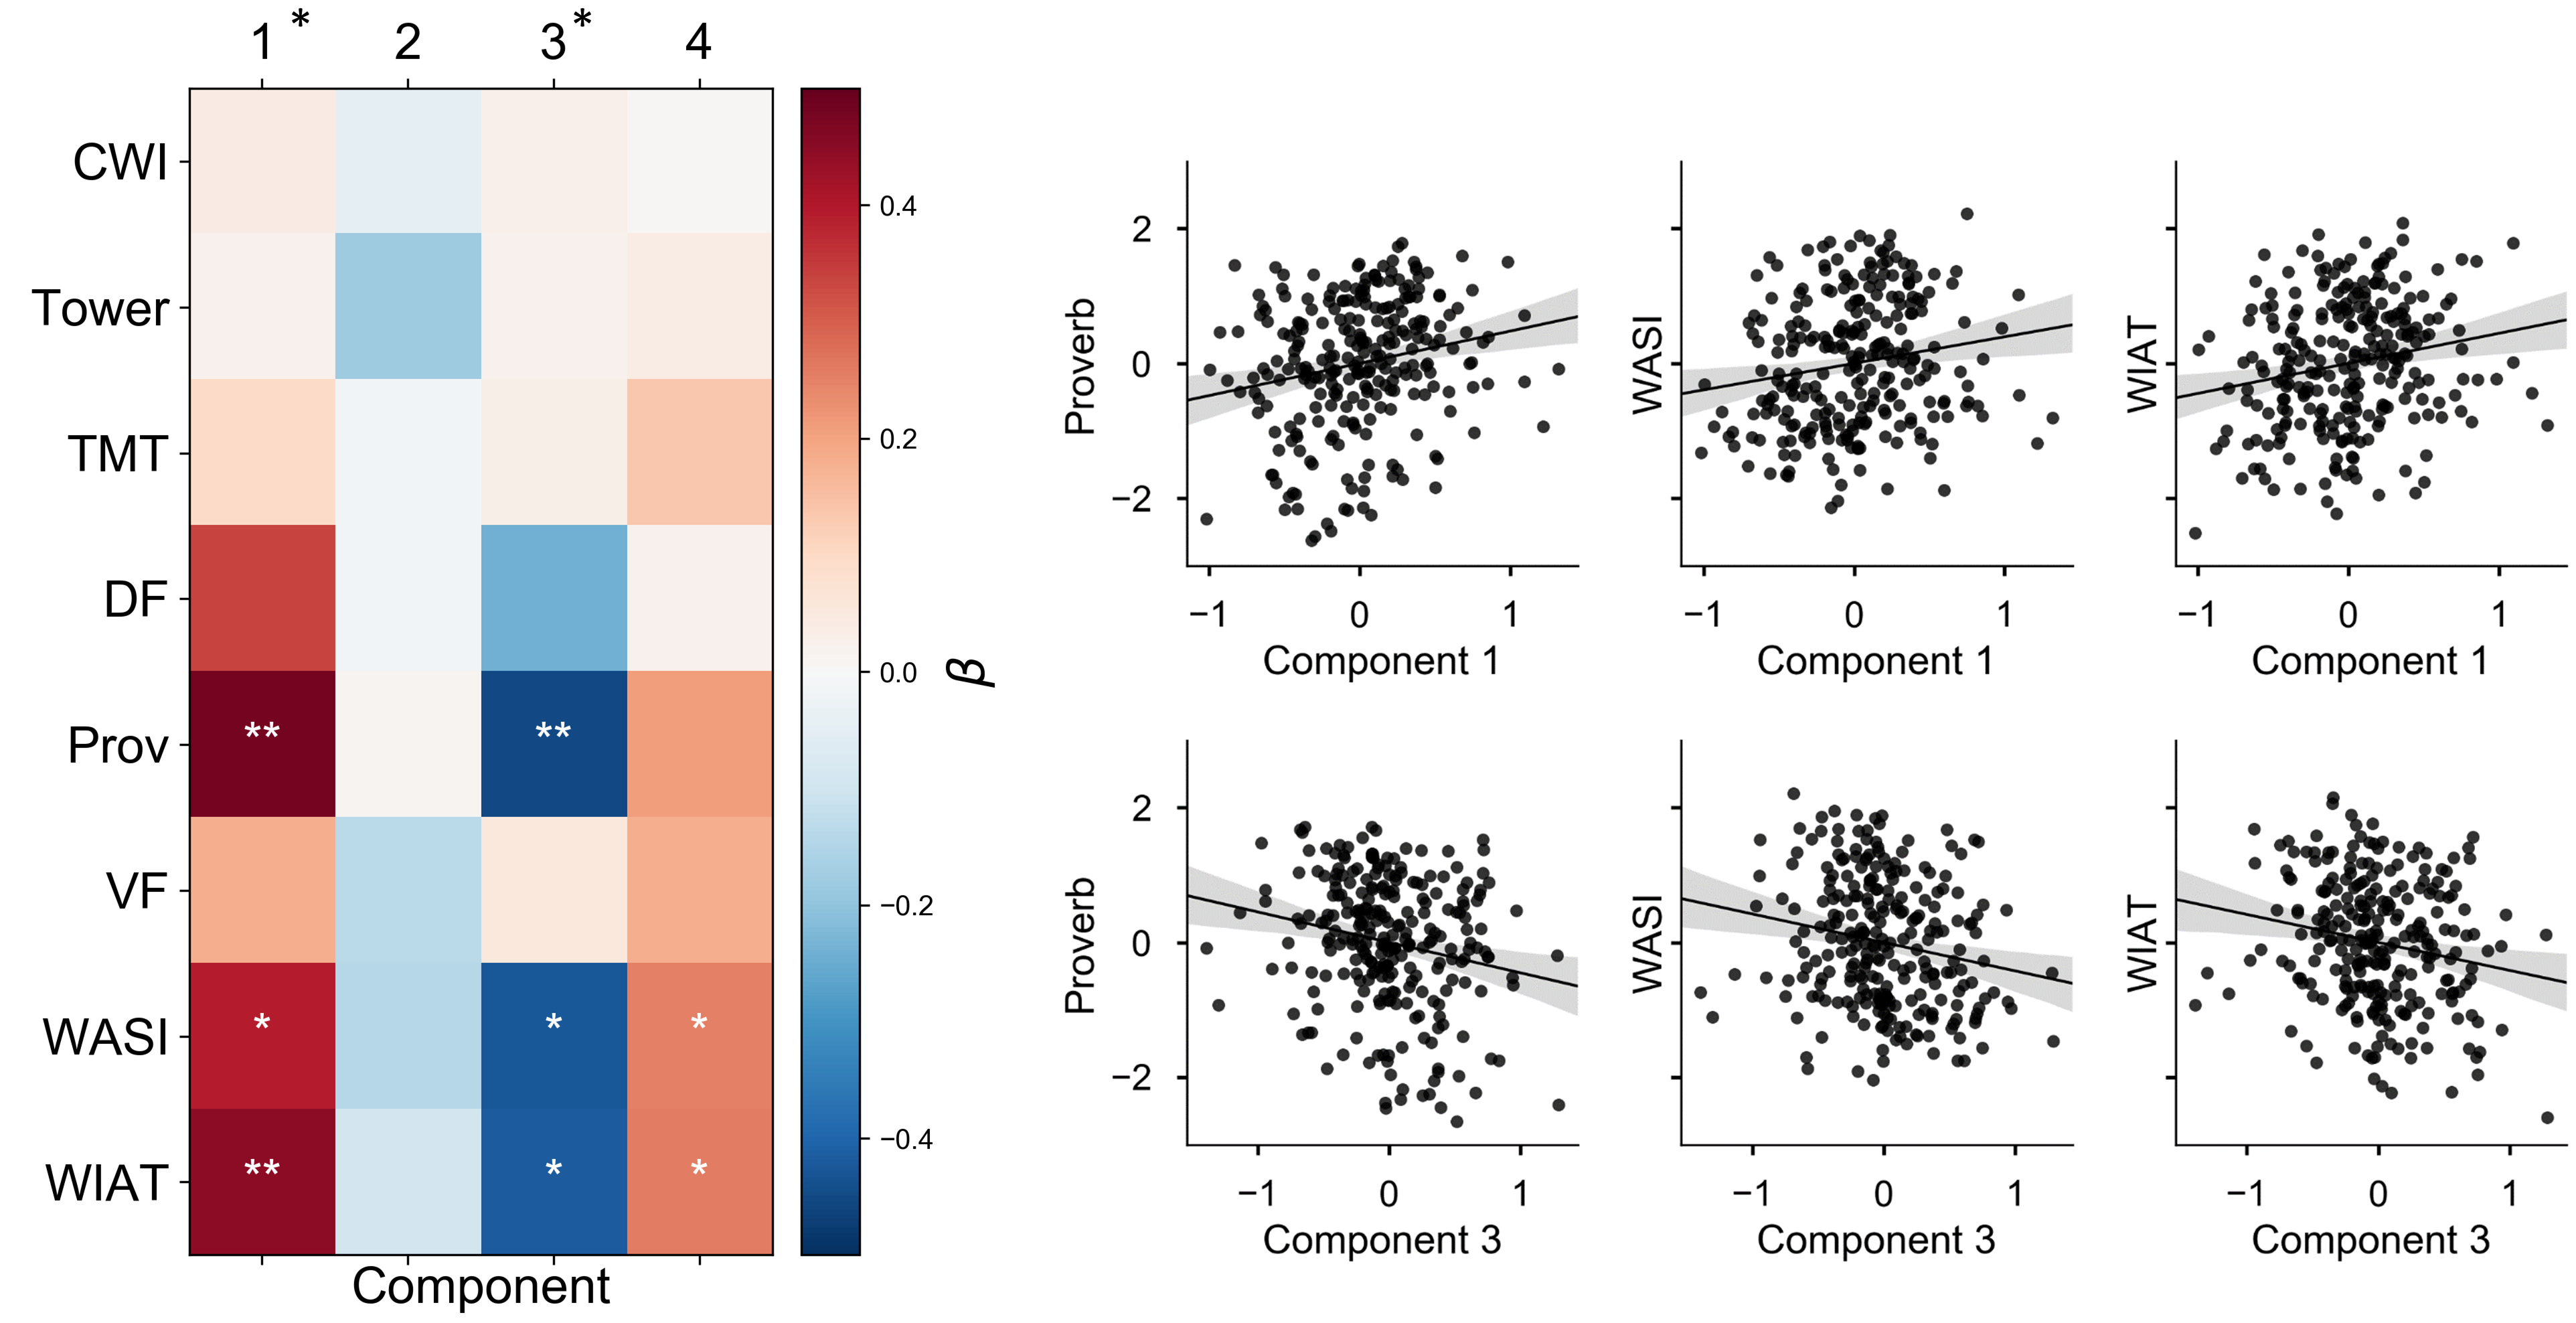
\includegraphics[width=0.8\textwidth]{chapters/img/study2fig3.png}
    \caption{The relationship between the different neural-cognitive components and the measures assessed in the cognitive battery.} 
    \caption*{
    \footnotesize{
    The components 1 and 3 were significant at the multivariate level determined by multiple multivariate regression, indicated by the asterisk outside of the heat map. The cells with asterisk(s) indicates the significant resluts from the univariate test (bonferroni corrected) and the parameter estimates for each variable. CWI – Colour-word interference, DF – Design fluency, Pro- Proverbs, TOW – Tower of London, TMT – Trail making task, VF- Verbal Fluency, WASI – Wechseler Adult Intelligence Test, WIAT – Weschler Individual Attainment Test. P-value significant codes:  0 ”***” 0.001 ”**” 0.01 ”*” .}
    }
    \label{fig:study2:fig3}
\end{figure}

Finally, we performed a simple principle component analysis on the eight task measures to explore the associations between experience and the structure of the laboratory data. The aim of this analysis was to see if the pattern retrieved from the univariate level in the previous multiple multivariate regression was related to the internal structure of the data. Component selection was determined based on the scree plot, and we accepted one component explaining 39\% of the variance. The principle component loaded on the intelligence measures and the proverb test. We fitted a linear model to this data to understand the relationship to the four canonical components. The results are reported in Figure 4. The overall linear model was significant (F(4, 253) = 5.43, p = .0003). In the linear regression model, Component 1 (β = 0.82, t(253) = 3.5, p = . 001, 95\% CI [0.36 1.29]) showed significant contribution to explaining the task principle component. Component 3 showed a negative correlation to the task components (β = -0.69, t(253) = -3.04, p = .003, 95\% CI [-1.13 -0.24]). The relationships between tasks and the neuro-cognitive components here were similar to the ones uncovered by the multiple multivariate regression. In this analysis Component 4 (β = 0.442, t(253) = 3.09, p = .002, 95\% CI [0.16 0.72]) showed a significant contribution in the regression model, but it did not pass the permutation test of robustness (p = 0.998). The related results should be treated cautiously. Together with our prior analysis, these results suggest that Components 1 and 3 are the most robust components identified in our study.

 \begin{figure}
    \centering
    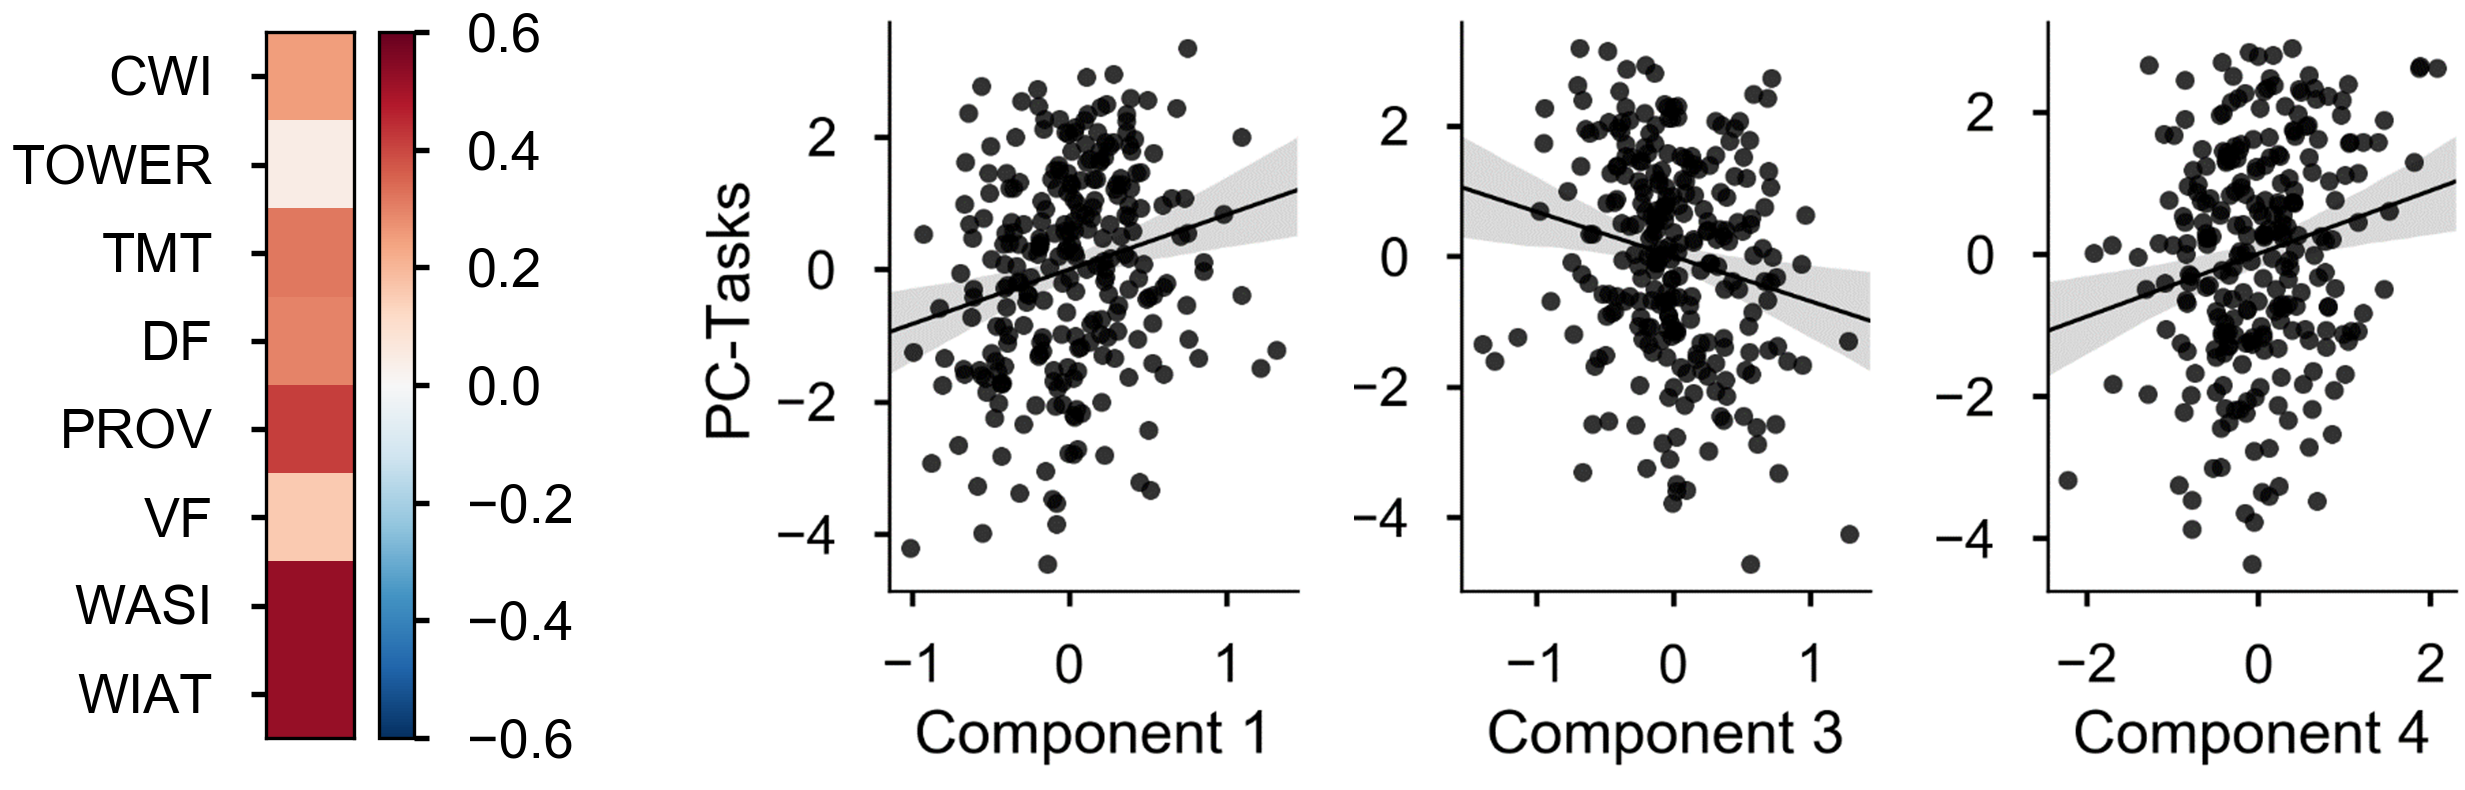
\includegraphics[width=0.8\textwidth]{chapters/img/study2fig4.png}
    \caption{The principle component and its relationship to the different neural-cognitive components.} 
    \caption*{
    \footnotesize{The heat map describes the principle component of the task battery, and the scatter plots describe the association with the components identified in our study. Component 1 and 3 passed the permutation test for component robustness significantly contributed in explaining the principle component of the task. Component 4 showed a significant contribution in the regression model, but it did not pass the permutation test. The related results should be treated cautiously.}
    }
    \label{fig:study2:fig4}
\end{figure}
% ==========================================================================================================

\section{Discussion}
\label{study2:discussion}
We set out to describe different modes of neuro-cognitive patterns derived through the simultaneous decomposition of whole brain connectivity data with self-reports of on-going experience. We used a whole brain parcellation that describes cortical function in seven independent networks \cite{Yeo2011}. 
We combined this data with self-reports of the experience of our participants at rest, using a multivariate approach that allows for the possibility of many-to-many mappings between neural patterns and on-going cognition. Our analyses identified four stable canonical components, describing unique dimensions of neural-experiential variation. Permutation testing demonstrated the statistical robustness of Components 1-3. Furthermore, two components (1 and 3) described independent patterns of performance in a battery of commonly used cognitive measures. This association with cognitive performance that establishes a source of independent validity for these neuro-cognitive components since they are related to independent measures of cognitive performance. We next consider the fit between the dimensions produced by our analysis and theoretical views of unconstrained neuro-cognitive processing.

We found evidence broadly consistent with contemporary representational accounts of unconstrained processing. The neural patterns described by Component One reflect a pattern of reduced correlation between regions with links to memory and representation (e.g. limbic, default mode) from those with links to external behaviour (e.g. visual and sensorimotor cortex and attention networks). This pattern was associated with experiences characterised by a sense of purposefulness, and with verbally mediated content that was social and temporal in nature. Participants high on this dimension were proficient at generating abstract semantic links and performed well on measures of reasoning and intelligence. Together the features of Component One support the hypothesis that the functional decoupling of systems important for memory and representation are important for aspects of unconstrained cognition \cite{Smallwood2013}. 
This capacity may arise from the topographical organisation of the cortex, in which neural systems that can take on more transmodal properties tend to be located in regions that are more distant in functional and structural terms \cite{Buckner2013,Margulies2016,Mesulam1998}. 
This spatial location may allow neural signals in these regions to take on properties that are discrepant from the neural signal more closely tethered to inputs describing the external world \cite{Buckner2013,Friston2013}. 
The pattern identified by Component One, therefore, may reflect a pattern of population variation describing the hypothesised role of functional decoupling of memory and representational systems plays in the generation of more abstract aspects of human cognition \cite{Margulies2016,Mesulam1998}. 
Importantly, in our prior work, limbic and default mode networks were the most distant in functional connectivity terms from unimodal systems \cite{Margulies2016}.
Our data also highlights neural patterns that capture the hypothesised influence of attention and control on on-going thought \cite{McVay2009}. 
Component 3 highlights links between reduced connectivity within attention and control systems and patterns of thought that emphasise personal importance. This is associated with worse performance on measures of intelligence and reasoning. The combination of a focus on personally important themes linked to poor performance on measures of general aptitude, captures the hallmark psychological features of the current concerns X executive-failure accounts of on-going thought \cite{McVay2009}. 
This view suggests that failures in attentional control lead to highly personally relevant cognition to intrude into ongoing thought, leading to lapses in task performance. Importantly, the neural pattern described by this component emphasises dysregulated connectivity both within and between networks implicated in attention and control by task-based studies \cite{Duncan2010}. 
Our prior work established that spontaneous mind-wandering is linked to cortical thinning within regions linked to attention and control, such as the intra-parietal sulcus \cite{Golchert2017}. 
Spontaneous mind-wandering has been linked to worse cognitive control \cite{Robison2018}, 
as well as showing stronger links with attention related problems, including ADHD \cite{Seli2015}. 
Together with these prior studies, our data suggests that population variation in the intrinsic neural functioning within networks with an established role in external task performance captures the hypothesised contribution of executive-failure to patterns of on-going thought.

The method of decomposition used in the current study also highlighted patterns related to affective processing and the modality of the experience that are similar to those seen in our prior work that applied principal components analysis (PCA) to self-reported data only. Component Four places experiences with visual features (“images”) in opposition to experiences with verbal features (“monologue”), capturing dissociations between visual and verbal thinking observed in our prior studies \cite{Konishi2015,Medea2016,Smallwood2016}. 
The accompanying neural pattern were associated with higher connectivity between the visual network with other networks, in particular the limbic system. It is important to note that our permutation analysis failed to validate this component, so despite its association with task performance using the PCA analysis it should be treated with relative caution. Component Two loads on emotional experiences (“cheerfulness”, “anger”, “guilt” and “happiness”) with the exception of those that are unhappy (“sad”). In neural terms this component was characterised by high levels of connectivity, however, unlike Component Four, this was highest between limbic and ventral attention networks. This pattern of coupling is consistent with accounts that emphasise interactions between saliency and limbic systems in affective processing \cite{Touroutoglou2012}. 
In the case of Component Two permutation testing indicated this component was likely to be robust in statistical terms, however, we did not observe associations with task performance. As with Component Four, interpretations of Component Two should be made with caution in lieu of more empirical work. 

Before closing it is worth considering several important limiting factors of our study. We focused on patterns of population variance in unconstrained neuro-cognitive processing that were measured once in each individual. Our study, therefore, cannot separate the influences state and traits on our observed components. Treating patterns of unconstrained processing as a trait is common in both the psychological \cite{McVay2009,Smallwood2013a} 
and neural domains \cite{Smith2015}. 
Nonetheless, it remains an open question how consistent these components will be across individuals over time, as well as which aspects may be better described as traits. Importantly, by its very nature there are dimensions of experience that our study cannot adequately address. We cannot, for example, identify brain-experience associations that are highly dynamic in nature and in particular those that change rapidly within an individual. Insight into this issue could be achieved by a focus on dynamic rather than static connectivity \cite{Kucyi2017}. 
For example, the application of techniques such as sliding window analysis \cite{Chang2010}%(Chang \& Glover, 2010) 
or Hidden Markov models \cite{Vidaurre2017} 
to fMRI could provide information that would complement our analyses. However, it may also be more important to examine these across multiple sessions within the same individuals, as this would also make it most possible to dissociate state from trait related influences on neural activity \cite{Mueller2013}%(Mueller et al., 2013). 
There are also types of experience that may be difficult to assess using the measure of retrospective experience sampling we have employed \cite{Smallwood2015}. 
For important features of experience, such as whether it has evolving features \cite{Mills2018}, 
or when the participant is unaware of the content of their experience \cite{Schooler2002}%(Schooler, 2002), 
these experiential features may be best assessed using experience sampling techniques that capture momentary elements of experience \cite{Smallwood2013PsychologicalBulletin}. %Smallwood 2013 Psychological Bulletin  

There are a number of methodological improvements that could enhance future studies of brain-experience association. A recent benchmark study by Ciric and colleagues \cite{Ciric2017}%(Ciric et al., 2017) 
shows that scrubbing can improve the performance of resting state analyses. Regarding to the analysis pipeline, we gained hyper-parameters and best model with nested-CV an approach that can help prevent overfitting \cite{BzdokYeo2017}.%(Bzdok & Yeo, 2017). 
There are also alternative ways that could provide better tests of the robustness of the components we identified. We assessed the validity of the components in three different ways; 1) with a data-driven, non-parametric permutation test \cite{Smith2015}%(Smith et al., 2015) 
that establishes the statistical validity of the identified components and 2) by establishing the relationship between the laboratory cognitive measures and 3) by consideration of their links with contemporary theoretical accounts of ongoing cognition. In our study, Components 1 and 3 were statistically significant in both cases and fitted well with contemporary accounts of ongoing cognition. Accordingly we place encourage readers to focus on these patterns from our data. There are alternative strategies that could help validate the robustness of patterns of brain-experience association. One approach could be to compare the relationship between multiple sessions within the same individual \cite{Poldrack2015}%(Poldrack et al., 2015) 
and to have a larger sample that would allow the reproducibility of these results through a formal split-half validation procedure. To achieve this latter aim for future studies, we have placed the questionnaire measure used in this study along with an example self-report collection task on GitHub at the following address: \url{https://github.com/htwangtw/restingstate_thoughtreports}. 
We encourage interested investigators to apply these measures in their resting-state investigation and to also upload the resultant data onto open fMRI. These studies could be used in conjunction with the openly access data used in this study to enable future investigations the opportunity to cross validate experiential analyses in a more sophisticated manner than we have been able to achieve in this study. The analysis pipeline of the current study can be further unified into one frame work that benefits from both validation strategies. We can include the number of components along with penalty coefficients in the hyper-parameters determined in the CV process, or determine the best penalty terms with the first component. The permutation test will then identify the reliable components occurring above chance level. After all the data-driven component selection, we can examine the survived components through their relations with well-documented cognitive measures and conclude the meaningful patterns. Finally, it is likely that our measure of on-going thought lacks important questions regarding the content of experience. It will be important, therefore, in the future to examine the relationships of the type described in this study with a more exhaustive description of on-going experience. We hope that by publishing our questionnaire collection task in a GitHub repository we will be able to harness the power of the broader community to help generate and test plausible questions for use in future studies.

% ==========================================================================================================

\chapter{Study 3}
\chaptermark{Study 3}
\label{ch:study3}
%\setcounter{equation}{0}

\newpage
%Abstract


% ====================================================================================================================
\section{Introduction}
\label{study3:intro}

% ==========================================================================================================

\section{Method}
\label{study3:method}
\subsection{Participants}
\label{study3:method:a}
Two hundred and seven healthy participants were recruited from the University of York (132 females, 65 males; age range = 18–-31 years, \textit{M} = 20.21, \textit{SD} = 2.36). 
This analysis included two data sets with some shared measurements and same MRI protocol as \ref{ch:study1}. 
Participants were right-handed native English speakers with normal or corrected-to-normal vision and no history of psychiatric or neurological illness. Participants underwent MRI scanning, completed an 1-hr online questionnaire. The first cohort is identical to the sample in \ref{ch:study1}. Participant attended three 
(165 participants; 99 females, 66 males; age range = 18–-31 years, \textit{M} = 20.43, \textit{SD} = 2.63) 2-hr behavioral testing sessions to complete a battery of cognitive tasks. 
The second cohort (42 participants; 33 females, 9 males; age range = 18–-23 years, \textit{M} = 19.79, \textit{SD} = 1.37) underwent two 2-hr behavioural testing sessions to complete a battery of cognitive tasks. The behavioural sessions took place within a week of the scan. Ten participants were excluded from the multivariate pattern analysis because they failed to complete all of the behavioural testing sessions. In total, 197 participants (126 females, 71 males; age range = 18–-31 years, \textit{M} = 20.11, \textit{SD} = 2.24) were included in the multivariate pattern analysis and the comparison with cognitive performance. Participants were rewarded with either a payment of \pounds 10 per hour or a commensurate amount of course credit. All participants provided written consent prior to the fMRI session and the first behavioural testing session. Approval for the study was obtained from the ethics committee of the University of York Department of Psychology and the University of York Neuroimaging Centre.

\subsection{MRI acquisition}
\label{study3:method:b}
The MRI acquisition protocol was identical to Chapter \ref{ch:study1}. Please refer to section \ref{study1:method:b} for details.

\subsection{Resting state data preprocessing}
\label{study3:method:c}

All preprocessing and denoising steps for the MRI data were carried out using the SPM software package (Version 12.0) and Conn functional connectivity toolbox (Version 17.f), based on the MATLAB platform (Version 17.a). The first three functional volumes were removed in order to achieve steady state magnetisation. The remaining data was first corrected for motion using six degrees of freedom (x, y, z translations and rotations), and adjusted for differences in slice-time. Subsequently, the high-resolution structural images were co-registered to the mean functional image via rigid-body transformation, segmented into grey/white matter and cerebrospinal fluid probability maps, and all functional volumes were spatially normalized to Montreal Neurological Institute (MNI) space using the segmented images and a priori templates. This indirect procedure utilizes the unified segmentation–normalization framework, which combines tissue segmentation, bias correction, and spatial normalization in a single unified model. No smoothing was employed, complying with recent studies that report the negative influence of this procedure on the construction of connectivity matrices analysis. 

Moreover, a growing body of literature indicates the potential influence of participant motion inside the scanner on the subsequent estimates of functional connectivity. In order to ensure that motion and other artefacts did not confound our data, we have employed an extensive motion-correction procedure and denoising steps, comparable to those reported in the literature. In addition to the removal of six realignment parameters and their second-order derivatives using the general linear model (GLM), a linear detrending term was applied as well as the CompCor method that removed five principle components of the signal from white matter and cerebrospinal fluid. Moreover, the volumes affected by motion were identified and scrubbed based on the conservative settings of motion greater than 0.5 mm and global signal changes larger than z = 3. Though recent reports suggest the ability of global signal regression to account for head motion, it is also known to introduce spurious anti-correlations, and was thus not utilised in our analysis. Finally, a band-pass filter between 0.009 Hz and 0.08 Hz was employed in order to focus on low frequency fluctuations.

\subsection{ROI-ROI functional connectivity.}
\label{study3:method:d}
We adopted a set of 57 regions based on the Yeo 7 networks. We split the networks into two hemispheres and extracted clusters. Two voxels are considered connected only if they are adjacent within the same x, y, or z direction. This yielded 57 clusters from the Yeo 7 networks parcellation. The implementation of spatial clusters extraction was retrieved from python library Nilearn \cite[ \url{http://nilearn.github.io/}, version 0.3.1]{Abraham2014}. Fully-connected, undirected and weighted matrices of bivariate correlation coefficients (Pearson's r) were constructed for each participant using the average BOLD signal time series obtained from all the 57 ROIs described above. The off-diagonal of each correlation matrix contained 1596 unique region-region connection strengths (i.e., the upper or lower triangle of the network covariance matrix). This approach provided a measure of connection strength of the whole brain for each participant. Finally, Fisher’s r-to-z transformation was applied to each network covariance matrix. 

\subsection{Behavioural data}
\label{study3:method:e}

\subsubsection{Cognitive tasks}
We selected X cognitive tasks that are common across the two cohorts and related to the previous literature on mind wandering. The selected tasks includes blah blah. Please refer to Appendix \ref{appendix:study1:subsection2} for the detailed description of the tasks.

\subsubsection{Experience sampling}
Please refer to Chapter \ref{ch:study1} section \ref{study1:method:d} for the experience sampling data collection and Table \ref{tab:study1:1} for the detailed questions. 

We did a PCA on the same thought probes to understand the relation within the reports.


\subsection{Multivariate pattern analysis}
\label{study3:method:f}
\subsubsection{SCCA}
We performed a sparse canonical correlation analysis \cite<SCCA; see>{Hastie2015}%{ Hastie, Tibshirani, \& Wainwright, 2015} 
on the functional connectomes and the cognitive tasks, to yield latent components that reflect multivariate patterns across neural organisation and cognition \cite<For similar application, see>{Wang2018}%Wang et al., 2017). 
SCCA maximised the linear correlation between the low-rank projections of two sets of multivatiate data sets with sparse model to regularise the decomposition solutions a process that helps maximise the interpretability of the results. The regularisation function of choice is L1 penalty, which produces ‘sparse’ coefficients, meaning that the canonical vectors (i.e., translating from full variables to a data matrix’s low-rank components of variation) will contain a number of exactly zero elements. L1 regularisation conducted (i) feature selection (i.e., select only relevant components) and (ii) model estimation (i.e., determine what combination of components best disentangles the neuro-cognitive relationship) in an identical process. This way we handle adverse behaviours of classical linear models in high-dimensional data. A reliable and robust open-source implementation of the SCCA method was retrieved as R package from CRAN 
\cite<PMA, penalized multivariate analysis, version 1.0.9>{Witten2009a}%(PMA, penalized multivariate analysis, version 1.0.9, Witten, Tibshirani, \& Hastie, 2009).
The amount of L1 penalty for the functional connectomes and cognitive task performance were chosen by cross-validation. The procedure is described below. 

\subsubsection{Model Selection}
The model selection process was conducted with two parts: 1) hyperparameter selection 2) mode selection. For the hyperparameter, L1 penalties for the left and right hand side, we performed a grid search on all possible penalty coefficients combination with cross validation on the explained variance of the first mode. The objective is determined by the best out-of-sample explained variance of the first mode. We decompose the full dataset with the selected hyper-parameters. Permutation tests with family-wise error correction \cite{Smith2015} was applied to access the mode(s) that occure above chance. 

\subsection{Group analysis}
\label{study3:method:g}

To determine how patterns of unconstrained neuro-cognitive activity related to performance on the self-report experience, we conducted an independent statistical analysis on the identical subjects. A Type III multivariate multiple regression with Pillai's trace test was applied to 5 individual scores for each of the latent components describing the neuro-cognitive mechanism from the SCCA were the independent variables, and the 13 measures from MDES were the dependent variables that we hoped to described by the linear combination of the latent components. Pillai's trace test is considered to be the most powerful and robust statistic for general use \cite{Huberty2006}.
The p-values reported were based on Bonferroni correction. The analysis was conducted in R (version 3.3.1). The multivariate multiple regression was conducted in R (version 3.3.1) using function ‘Manova’ in R package ‘car’ (companion to applied regression, version 2.1–5).


% ==========================================================================================================

\section{Results}
\label{study3:results}

\subsection{Determining constituent category of cognitive functions}
% grid search results
% permutation test results
% explain the significant components

\subsection{The relationship between neuro-cognitive components and self-reports on thoughts}
% multivariate main effect
% univariate main effects shows resemblance to the PCA

% ==========================================================================================================

\section{Discussion}
\label{study3:discussion}

\chapter{General Discussion}
\chaptermark{Discussion}
\label{ch:discussion}
%\setcounter{equation}{0}
% ==========================================================================================================

Donec diam ligula, gravida a dignissim nec, iaculis id tellus. Aliquam accumsan, tortor sodales imperdiet condimentum, elit nibh condimentum sem, sit amet ullamcorper odio lectus ut mi. Ut lobortis sollicitudin sodales. Phasellus et leo orci, eget consectetur elit. Maecenas convallis justo vitae elit blandit congue. In ut mauris ac massa suscipit tincidunt mattis at sem. Vivamus cursus auctor fermentum. Praesent et bibendum nibh. Mauris at diam libero, sit amet tincidunt est. Donec eu ante velit, sit amet rutrum eros. Cras aliquam, quam ut auctor viverra, ante justo ultrices massa, quis aliquam arcu augue quis augue. Aliquam vulputate, arcu at cursus aliquet, eros nisi eleifend augue, a imperdiet metus quam at risus. Nullam tellus mauris, vulputate id egestas eget, consequat non odio. Mauris sem risus, convallis vel tempor id, lacinia vel magna. Integer erat mi, semper quis posuere ut, consectetur a diam. Integer risus velit, consectetur nec vehicula id, tincidunt vel nunc. Etiam ac lorem quis diam varius congue.
% ====================================================================================================================
\section{Structure of this chapter}
\label{ch7:structure}
Nullam non ligula quis dui feugiat egestas. Praesent consequat sapien sed arcu ultricies gravida. Duis non odio nibh. Nulla placerat, dolor ac sollicitudin convallis, nunc leo rutrum justo, ut congue arcu libero id metus. Suspendisse potenti. Etiam sagittis felis et est semper at dictum dolor elementum. Aenean rhoncus blandit nisl, at adipiscing metus sagittis non. Quisque feugiat lacus at augue egestas consectetur. Cras eget egestas dui. Integer congue iaculis iaculis. Vivamus rhoncus magna et neque interdum sit amet dictum velit sollicitudin. In ut sapien a orci tincidunt sagittis. Sed justo arcu, tincidunt ac tincidunt vitae, aliquet sed libero. Aenean vel tellus eget dui varius fermentum vitae sit amet lectus.

% ==========================================================================================================

\section{The first section}
\label{ch7:first}
Integer vulputate vulputate imperdiet. Integer varius elementum urna id hendrerit. Nulla vitae ante leo, id tincidunt purus. Praesent quam lacus, semper vitae tristique pulvinar, gravida sit amet sem. Sed porttitor orci nec orci sodales ac malesuada felis consequat. Aliquam erat volutpat. Cras dapibus dignissim neque non convallis. Ut quis tellus arcu, vitae fermentum orci. Nunc pharetra leo at odio posuere ac pretium odio blandit. Nulla pellentesque tincidunt gravida. 

Phasellus quis metus vel lectus porta vehicula ut eu felis. Mauris libero velit, egestas vel tempus eget, iaculis sit amet magna. Proin accumsan semper consectetur. Nulla et euismod augue. Proin lacus sapien, convallis nec placerat at, vulputate eu massa. Etiam nisi dui, consequat in consequat eget, posuere vel velit. Mauris accumsan venenatis facilisis.

\subsection{The first subsection}
\label{ch7:first:a}
Aliquam imperdiet est id nulla fringilla vel luctus tellus pretium. Aliquam tincidunt ante nec lacus ullamcorper placerat. In bibendum, turpis vitae dapibus interdum, elit quam tempus nisi, ac vestibulum nulla nisl vel mauris. Nullam ut diam nisi. Vestibulum vitae eros sed felis fermentum ultrices. Integer tincidunt, justo vel luctus gravida, leo erat placerat ipsum, sit amet condimentum diam massa ac ligula. 

Etiam nec ullamcorper lectus. Quisque auctor libero facilisis risus volutpat vitae auctor felis fermentum. Mauris non sapien eget metus laoreet lacinia eget ac magna. Sed sed leo leo. Curabitur in est at quam condimentum semper sit amet sed ipsum. Nam neque est, auctor posuere varius ac, bibendum sit amet urna. 

Nunc lobortis tortor id orci molestie pulvinar suscipit ipsum mattis. Maecenas auctor mi mauris. Nunc condimentum lectus eu libero ornare commodo. Mauris cursus felis quis nunc ornare a blandit sem commodo. Vestibulum eu neque ut est hendrerit condimentum. Ut nisl mi, tristique ut malesuada aliquet, imperdiet a quam. Nam malesuada accumsan massa, sit amet ullamcorper ante mattis at.

\subsection{The second subsection}
\label{ch7:first:b}
Donec nec arcu lacus, ut dictum purus. Suspendisse tristique turpis vitae enim semper non facilisis ligula posuere. Nulla nulla arcu, pharetra eget bibendum consectetur, eleifend ut tellus. Proin ac tortor erat, quis facilisis leo. Nulla sit amet tellus eu sapien tempus tempor. Vestibulum vehicula lacinia dui non iaculis. 

Pellentesque massa velit, mollis eu lacinia euismod, bibendum sed purus. Duis neque enim, accumsan id euismod ac, pharetra iaculis justo. Cras volutpat, massa id ullamcorper aliquam, ligula dui ultricies libero, id tristique justo magna ac lectus. Suspendisse et aliquet tortor. In non nisl orci, id volutpat odio. 

Maecenas condimentum tincidunt nunc, vitae convallis metus tristique eget. Ut vel mi sed eros sagittis dapibus. Maecenas nibh purus, eleifend vel vulputate in, vehicula at dui. Fusce nec nunc tellus, ac vehicula risus. Aenean semper ligula vitae nisl volutpat tincidunt. Sed id erat vel leo dapibus commodo eget sit amet turpis. Mauris sed eros ac magna egestas volutpat ut a dui. Lorem ipsum dolor sit amet, consectetur adipiscing elit.

\subsection{The third subsection}
\label{ch7:first:c}
Curabitur volutpat dictum arcu nec porta. Praesent nec nunc at dolor faucibus laoreet. Sed sollicitudin nisl et urna auctor nec aliquam ipsum auctor. Morbi elementum tortor non sapien ultricies sed lobortis augue fermentum. Suspendisse elit nisl, scelerisque nec iaculis vel, rutrum lobortis tellus. Fusce porta, justo eu venenatis tincidunt, purus lorem malesuada orci, in gravida est nisl a massa. Ut facilisis felis a ante rhoncus gravida mollis felis mattis. Etiam convallis augue sit amet magna tristique tristique. 

Aliquam imperdiet magna at sem adipiscing quis elementum nunc tincidunt. Nulla facilisi. Donec vitae tellus lectus. Proin dapibus ornare scelerisque. Suspendisse mollis massa vitae sapien volutpat feugiat. Vivamus eu est id diam sollicitudin viverra. Donec sit amet ipsum mauris, eget semper augue. In blandit viverra lobortis. Curabitur lacinia pharetra tincidunt. Etiam porttitor orci quis diam molestie pretium. Ut vel nisi odio, et condimentum sem.

\subsection{The fourth subsection}
\label{ch7:first:d}
Maecenas eu massa ac quam congue congue sed ac lorem. Nulla luctus libero id massa faucibus id ornare elit scelerisque. Maecenas adipiscing gravida arcu, non adipiscing dolor sagittis sit amet. Curabitur tristique odio at nisi consectetur cursus. Vivamus a nunc vel mauris ornare faucibus ut eget eros. Quisque egestas purus ac risus tempor non rhoncus odio sodales. 

Nulla tincidunt laoreet aliquam. Vestibulum ante ipsum primis in faucibus orci luctus et ultrices posuere cubilia Curae; Sed vel magna et nisl placerat semper. Praesent id nulla neque. Aenean tempor volutpat libero ac rhoncus. Integer sollicitudin est at enim lacinia molestie. Donec vel tincidunt magna. Integer iaculis semper vehicula. Lorem ipsum dolor sit amet, consectetur adipiscing elit. Mauris ullamcorper blandit libero ac commodo.

% ==========================================================================================================

\section{The second section}
\label{ch7:second}
Vestibulum ante ipsum primis in faucibus orci luctus et ultrices posuere cubilia Curae; Sed ut velit id velit condimentum feugiat. Pellentesque nibh enim, malesuada in laoreet non, dapibus ac metus. 

Morbi ultricies, orci nec convallis semper, diam metus varius nibh, quis ultrices neque libero sed metus. Duis mollis congue faucibus. Phasellus a augue non ligula commodo viverra eu vitae mi. 

Integer vehicula nunc lacus. Pellentesque nec lorem enim, vel molestie lorem. Donec a magna velit, quis tincidunt libero. Nulla facilisi. Maecenas interdum elit dui. Fusce sollicitudin faucibus pulvinar.

\subsection{The first subsection}
\label{ch7:second:a}
Aliquam imperdiet est id nulla fringilla vel luctus tellus pretium. Aliquam tincidunt ante nec lacus ullamcorper placerat. In bibendum, turpis vitae dapibus interdum, elit quam tempus nisi, ac vestibulum nulla nisl vel mauris. Nullam ut diam nisi. Vestibulum vitae eros sed felis fermentum ultrices. Integer tincidunt, justo vel luctus gravida, leo erat placerat ipsum, sit amet condimentum diam massa ac ligula. 

Etiam nec ullamcorper lectus. Quisque auctor libero facilisis risus volutpat vitae auctor felis fermentum. Mauris non sapien eget metus laoreet lacinia eget ac magna. Sed sed leo leo. Curabitur in est at quam condimentum semper sit amet sed ipsum. Nam neque est, auctor posuere varius ac, bibendum sit amet urna. 

Nunc lobortis tortor id orci molestie pulvinar suscipit ipsum mattis. Maecenas auctor mi mauris. Nunc condimentum lectus eu libero ornare commodo. Mauris cursus felis quis nunc ornare a blandit sem commodo. Vestibulum eu neque ut est hendrerit condimentum. Ut nisl mi, tristique ut malesuada aliquet, imperdiet a quam. Nam malesuada accumsan massa, sit amet ullamcorper ante mattis at.

\subsection{The second subsection}
\label{ch7:second:b}
Donec nec arcu lacus, ut dictum purus. Suspendisse tristique turpis vitae enim semper non facilisis ligula posuere. Nulla nulla arcu, pharetra eget bibendum consectetur, eleifend ut tellus. Proin ac tortor erat, quis facilisis leo. Nulla sit amet tellus eu sapien tempus tempor. Vestibulum vehicula lacinia dui non iaculis. 

Pellentesque massa velit, mollis eu lacinia euismod, bibendum sed purus. Duis neque enim, accumsan id euismod ac, pharetra iaculis justo. Cras volutpat, massa id ullamcorper aliquam, ligula dui ultricies libero, id tristique justo magna ac lectus. Suspendisse et aliquet tortor. In non nisl orci, id volutpat odio. 

Maecenas condimentum tincidunt nunc, vitae convallis metus tristique eget. Ut vel mi sed eros sagittis dapibus. Maecenas nibh purus, eleifend vel vulputate in, vehicula at dui. Fusce nec nunc tellus, ac vehicula risus. Aenean semper ligula vitae nisl volutpat tincidunt. Sed id erat vel leo dapibus commodo eget sit amet turpis. Mauris sed eros ac magna egestas volutpat ut a dui. Lorem ipsum dolor sit amet, consectetur adipiscing elit.

\subsection{The third subsection}
\label{ch7:second:c}
Curabitur volutpat dictum arcu nec porta. Praesent nec nunc at dolor faucibus laoreet. Sed sollicitudin nisl et urna auctor nec aliquam ipsum auctor. Morbi elementum tortor non sapien ultricies sed lobortis augue fermentum. Suspendisse elit nisl, scelerisque nec iaculis vel, rutrum lobortis tellus. Fusce porta, justo eu venenatis tincidunt, purus lorem malesuada orci, in gravida est nisl a massa. Ut facilisis felis a ante rhoncus gravida mollis felis mattis. Etiam convallis augue sit amet magna tristique tristique. 

Aliquam imperdiet magna at sem adipiscing quis elementum nunc tincidunt. Nulla facilisi. Donec vitae tellus lectus. Proin dapibus ornare scelerisque. Suspendisse mollis massa vitae sapien volutpat feugiat. Vivamus eu est id diam sollicitudin viverra. Donec sit amet ipsum mauris, eget semper augue. In blandit viverra lobortis. Curabitur lacinia pharetra tincidunt. Etiam porttitor orci quis diam molestie pretium. Ut vel nisi odio, et condimentum sem.

\subsection{The fourth subsection}
\label{ch7:second:d}
Maecenas eu massa ac quam congue congue sed ac lorem. Nulla luctus libero id massa faucibus id ornare elit scelerisque. Maecenas adipiscing gravida arcu, non adipiscing dolor sagittis sit amet. Curabitur tristique odio at nisi consectetur cursus. Vivamus a nunc vel mauris ornare faucibus ut eget eros. Quisque egestas purus ac risus tempor non rhoncus odio sodales. 

Nulla tincidunt laoreet aliquam. Vestibulum ante ipsum primis in faucibus orci luctus et ultrices posuere cubilia Curae; Sed vel magna et nisl placerat semper. Praesent id nulla neque. Aenean tempor volutpat libero ac rhoncus. Integer sollicitudin est at enim lacinia molestie. Donec vel tincidunt magna. Integer iaculis semper vehicula. Lorem ipsum dolor sit amet, consectetur adipiscing elit. Mauris ullamcorper blandit libero ac commodo.

% ==========================================================================================================

\section{Summary}
\label{ch7:summary}
Vivamus blandit varius accumsan. Maecenas in lectus in ipsum fringilla tempus id sit amet nulla. Curabitur congue imperdiet odio, vel laoreet nisl ullamcorper at. Praesent vel erat augue, vitae ullamcorper velit. Cras tempus, purus non pellentesque consequat, tellus nulla cursus dui, id porta ante leo nec dui. In eget nibh vitae libero congue gravida non a ipsum. 

Mauris ac nulla eros. Maecenas laoreet, enim ornare rutrum facilisis, augue neque iaculis lorem, id pulvinar nibh leo at nisi. Sed purus dui, sagittis quis fringilla et, placerat nec elit. Proin ultrices odio sit amet quam rhoncus mollis. Ut convallis ligula a ligula sodales ornare. Phasellus ultrices mauris ac tellus cursus porttitor. 

Aliquam aliquam, tortor sed facilisis interdum, sapien ipsum malesuada enim, quis mattis libero lectus non mi. Donec lacinia mauris sit amet risus sagittis sodales. Suspendisse id sapien ipsum. Etiam sit amet neque non mauris tristique mattis.

Nam lobortis tellus lacus, vitae dignissim est. Pellentesque habitant morbi tristique senectus et netus et malesuada fames ac turpis egestas. Maecenas eu risus massa. Ut at dui et sapien eleifend ultricies. Pellentesque habitant morbi tristique senectus et netus et malesuada fames ac turpis egestas. Nulla ullamcorper vehicula tempor. 

Donec turpis risus, luctus a suscipit sit amet, scelerisque sit amet libero. Morbi porta sollicitudin libero nec ornare. Curabitur semper tellus id urna dictum varius. Quisque at eros vitae elit pharetra tristique et sit amet enim. In ornare varius leo nec elementum. Duis elementum tellus in nisi ultrices sit amet vehicula dui faucibus. Aliquam vel elit id risus pulvinar pretium. 

Curabitur at mauris felis, quis varius dolor. Pellentesque habitant morbi tristique senectus et netus et malesuada fames ac turpis egestas. Aliquam id posuere lorem. Donec ut aliquet nisi.


% appendices
\cleardoublepage
% latex does not allow nested imports, so include all appendices in this file as a separate 'chapter'

\appendix
\setcounter{chapter}{0}

\renewcommand{\chaptername}{Appendix}
\renewcommand{\theequation}{\Alph{chapter}.\arabic{section}.\arabic{equation}}
\setcounter{equation}{0}
\addcontentsline{toc}{chapter}{\numberline{}Appendix}

% ==========================================================================================================

\chapter{Dimensions of Experience: Supplemental Materials}
\label{appendix:study1}
\textit{The following content has been adapted from the online supplemental material of: }\\
Wang, H.-T., Poerio, G. L., Murphy, C. E., Bzdok, D., Jefferies, E., \& Smallwood, J. (2018). Dimensions of Experience: Exploring the Ontology of the Wandering Mind. \textit{Psychological Science}, 29 (1), 56–-71. doi: 10.1177/0956797617728727
% ==========================================================================================================
\section{Questionnaires}
\label{appendix:study1:subsection1}

\subsection{Health Organization Adult ADHD Self-Report Scale}
This is a self-report screening scale of adult ADHD, developed by the world health organisation\cite{Kessler2005}. This questionnaire comprises 18 questions to access the frequency of DSM-IV Criterion A symptoms of adult ADHD. We take the average scores across all 18 questions to access the participants’ ADHD tendency.

\subsection{Autism Spectrum Quotient}
The Autism Spectrum Quotient \cite{Baron-Cohen2001} comprises 50 questions, included 10 questions measuring 5 different dimensions: social skills, attention switching, attention to detail, communication, and imagination. For each questions the participant has four options: definitely agree, slightly agree, definitely disagree, and slightly disagree. ‘Definitely agree’ or ‘slightly agree’ responses scored 1 point on half of the designated questions.  ‘Definitely disagree’ or ‘slightly disagree’ responses scored 1 point on the other half of the questions.  The scores of each dimension is calculated with the sum of the scores of designated the questions. 

\subsection{British Dyslexia Association Dyslexia checklist}
The British Dyslexia Association Dyslexia checklist \cite{Smythe2001} comprises 15 questions to access the tendency of dyslexic. Each answer of the questions have a designated scores. Individuals scoring less than 45 are probably non-dyslexic; individual scoring 45 – 60 shows a mild level of dyslexia; scoring above 60 suggests moderate or severe dyslexia. The score in the current study is the sum of the scores.  

\subsection{World Health Organization Quality of Life}
The World Health Organization Quality of Life \cite{WHOQOL2002} assessment measures the quality of life cross-culturally.  In the current study, a shorter version of the original instrument, WHOQOL-BREF, was used, as it is recommended for large research studies. WHOQOL-BREF comprises 26 questions. The assessment measure the following broad domains: physical health, psychological health, social relationships, and environment. The official scoring system can be obtained on request from the official website.  

\subsection{CES-Depression scale}
The CES-Depression scale \cite{Radloff1977} is a self-report scale designed to measure the symptoms of depression in the general population. The scale contains 20 questions accessing the frequency of depressive symptoms in the past one week. In the current study we used the sum of the scores as an indicator of depression.
 
\subsection{State-Trait Anxiety Inventory}
The State-Trait Anxiety Inventory \cite{Spielberger1987} is a measure of trait and state anxiety, composing with 20 state anxiety questions and 20 trait anxiety questions. The state anxiety questions measure the level of anxiety when taking the questionnaire; the trait anxiety questions measure the general level of anxiety. The questions are rated on a 4-point scale. Mean scores of the state and trait questions were taken as our measurement, where higher scores indicates a greater level of anxiety. 

\subsection{Ruminative Response Scale}
The Ruminative Response Scale \cite{Treynor2003} is a 22-question self-report measure of rumination. Rumination involves introverted focus on negative mood and was found associating with depressive symptoms and stress \cite{Moberly2008a}. The questions are rated on a 4-point scale. Mean scores of the questions were taken as our measurement, where higher scores indicates a greater level of rumination. 

% ==========================================================================================================
\section{Cognitive tasks}
\label{appendix:study1:subsection2}
The behavioural tasks were allocated into three sessions based on apparatus needed. Visual attention and generative semantic tasks were in session A, and semantic and episodic memory tasks were in session B and C. In each session, the first and second tasks were the mind-wandering task and the flanker task. In session B and C, the third task was the encoding and the delayed-recall phases of the word pair memory task respectively. The rest of the tasks were performed based on a pre-allocated order. 
\subsection{General apparatus of the laboratory session}
In session B and C, the participants were in a sound proofed booth with a big glass window for the testers to monitor them. There were four testing spaces separated by office screen dividers. The tasks were delivered on Windows 7 computers and presented on 21 inches LCD monitors. Headsets were given to participants to deliver audio stimulus and blocking distracting noises. Participants were instructed to view the screen from a distance of 65 cm. The participants raised their hand to inform the experimenter to start each task. In session A, the visual attention tasks were delivered on a Windows 7 computer and presented on a 21 inches CRT monitor in a small room with light switch. The generative semantic tasks were delivered on a Windows 7 computer and presented on a 21 inches LCD monitor and a headset with microphone attached were used to recording verbal responses. 
\subsection{Semantic tasks}
The tasks employed a 3 alternative force choice (3AFC) paradigm with the probe presented alongside the three choices among which the target was selected. There are four tasks: Relatedness Task (Word-to-Picture Matching; Word-to-Word Matching; Picture-to-Picture Matching), Identity Matching Task(Word-to-Picture Matching), Feature Matching Task, and Scrambled Picture Matching as the control task.

The unrelated distracters of each trial were selected among the targets from other trials ensuring that they were not linked to the probe. Except for the Feature Matching Task, all the tasks contain the same trial structure. Each trial started with 500ms blank screen. The three choices were subsequently presented on the bottom of the screen for 900ms. Finally the probe was presented on the top middle section of the screen. Probe and choices remained visible until participants’ response or for a maximum of 3 seconds. In the Feature Matching Task, the 500ms blank screen was replaced by the probe with, in bracket, the feature (cue) as criterion for the matching (colour, size, shape or texture). Probe and cue were presented for 1000ms. The three choices were subsequently presented on the bottom of the screen. Probe, cue and choices were presented as written words and remained visible until participants’ response or for a maximum of 3 seconds.

The stimuli employed in the tasks were selected from a larger dataset of words and photographs used in previous experiment
\cite{Davey2015, Krieger-Redwood2012, Krieger-Redwood2015, Whitney2012}. 
The pictures were coloured photographs collected on internet and re-sized to fit the trial structure (200pixel, 72 dpi). All the coloured pictures and words were rated for familiarity and imageability using 7-point Likert scales. Lexical frequency count for the words was obtained by the SUBTLEX-UK database \cite{VanHeuven2014}.

For the details of the design, please refer to the online supplementary material of \cite{WangPsychScience2018}.

\subsection{Fluency Task}
During Verbal Fluency \cite{Adlam2010,Balota2008}, participants had 1 minute to generate as many unique words as possible belonging to a semantic category (category fluency) or starting with a specific letter (letter fluency). Semantic fluency was assessed for six categories split in two blocks (Block A: fruits, vehicles, type of dogs; Block B: animals, tools, type of boats). Letter fluency was assessed for three letter cues (Block C: A, F, S). Block order was counterbalanced across participants and the order of cues within each block was randomized. Participants’ verbal responses were collected and the audio recordings were transcribed and scored off-line.

\subsection{Word pair memory task}
Participants also undertook a Word Pair Memory Task (WPMT) to assess episodic memory \cite{Cairney2016}. 80 words were selected from an adapted version of The University of South Florida (USF) word association, rhyme, and word fragment norms \cite{Nelson2004} to create 40 semantically unrelated cue and target word pairs (e.g. owl – frame). Both the cue and target words were singular and they were matched for concreteness (t(39) = 0.39; p = .696), lexical frequency (t(39) = -4.71; p =.640), word length (t(39) = 0.09; p =.933) and number of syllables (t(39) = -0.73; p = .472). There were no pre-existing forward or backward associated relationships between any of the words, reducing the likelihood of erroneous associations between words in separate pairs.\\
During an initial learning phase, participants were presented with the unrelated words pairs, one at a time for 5 seconds each. This encoding phase was followed by a recall phase during which they attempted to recall the second word from the first word in the pair, they had 12 seconds for each trial and received a feedback after each response. In case of no response or error the feedback included the correct match. Participants were required to reach a performance criterion of 60\% correct responses, with a maximum of three repetitions of the recall phase for the entire list of word pairs. In the subsequent behavioral testing session that took place at least one day apart, participants attempted to recall the pairs immediately (without feedback) and provided a confidence rate about each of their responses using a 7-point Likert scale. 

\subsection{Digit span}
For the Forward and Backward Digit Span Test we used the stimuli and the score procedure described in the WASI battery. For each trial, audio files of each digit were played in the sequential order reported in the WASI battery. The Forward and Backward Digit Span versions were tested in separate blocks and instructions were presented at the beginning of each block asking participants to listen to the sequence of numbers and type them in the same order, for the Forward block, or in reverse order for the Backward block. 

\subsection{Flanker task}
We used the flanker task paradigm developed by \cite{Eriksen1974} as a baseline executive measure in this study. This task is conducted at the beginning of each laboratory sessions. The target was an arrowhead at the centre, pointing to the left or right direction. This target was flanked on either side by two to four items. The items were arrows in the same direction (congruent condition), or in the opposite direction (incongruent condition), or lines (neutral condition). The participant’s task was to identify the direction of the centrally presented arrow by pressing the left arrow key for the left direction and the right arrow key for the right direction. The stimuli were white and displayed on a black background. Each trial lasted for 4000 msec. A trial started with a fixation period of 900 - 2100 msec and then the target and the flankers appeared simultaneously. The target and the flankers were presented until the participant responded but for no longer than 1700 msec.  After the participant made a response, the target and flankers disappeared immediately and then a post-target fixation cross was presented. The duration of the post-target fixation period was based on the duration of the first fixation and RT (4000 ms minus duration of the first fixation minus RT). After this interval, the next trial began. 
 
\subsection{Task-switching task}
\label{appendix:study1:subsection2:TS}
We used the task-switching paradigm developed by \cite{Mayr2000} and the design and task materials were constructed based on \cite{Whitmer2007}. This task measured executive control on inhibiting previously relevant information. In this task, the participant identified the spatial location of a deviant object with a verbal instruction cue. The participant used a number pad to respond. Number 1,2,4, and 5 were used. Each of them responded to the spatial location of the designated rectangle. In each trial, four blue rectangles arranged into a two-by-two matrix were displayed on screen. The rectangles can vary from each other on one of three dimensions: size, motion, or orientation. Before a set time interval of 100ms or 900ms, a verbal cue on dimensions appeared on the centre of the screen. There were one practice block and two experiment blocks. The cue-stimuli interval in the practice is 500 msec, and 900 msec and 100 msec respectively in the two experiment blocks. The trials are categorised into four: control, inhibitory, uncategorised switch and repeat, see \cite{Whitmer2007} for details. 

\subsection{Four mountains task}
We used the four mountains task developed by \cite{Hartley2007} as a measure of spatial scene construction memory. In this task, the participant identified the target image that match the topography of the sample image across 30 trials. The participant was presented with a sample image of four mountains for 10 seconds, and then a four-choice of landscapes arranged in a two-by-two grid shown on the screen. The participant had no limit on thinking time for each trial, and they pressed number 1 to 4 to select the image. The target image is the same landscape as the sample image, but the perspective and environment (lighting, weather and vegetation) is changed. 

\subsection{Ravens advanced progressive matrices}
The Ravens Advanced Progressive Matrices \cite<RAPM>{Raven1998} measured ‘educative ability’ – that is the ability to make sense and meaning out of complex non-verbal stimuli. In order to complete the task participants were tasked with finding new patterns and relationships between the stimuli. The RAPM used in the current study contained two tests: (i) practice test - containing 2 problems and (ii) the full test – containing 36 problems. For each problem a set of 9 boxes (ordered in a 3x3 design) were shown on the screen. All but one box contained a pattern. At the bottom of the screen were 4 additional boxes, each containing a unique pattern. Participants were required to select out of these 4 potential boxes which pattern should go in the empty box. During the practice phase participants were given online feedback outlining whether their response was correct and, if not, how they should decide which box was the correct answer. If participants had any further questions, then they were instructed to ask the experimenter before starting the main experiment. During the full test no feedback was given. Participants were given 20 minutes to complete as many problems as they could, the problems got progressively more difficult.

\subsection{Unusual uses task}
The Unusual Uses Task \cite{Guilford1967} assessed divergent thinking and creativity. Participants were instructed to list as many unusual uses as they can for a familiar object. Three objects were selected (newspaper, brick and shoe). Uses were considered ‘unusual’ if they were not the original use of the item. For example, saying ‘crosswords’ for newspaper would not be considered unusual, however saying ‘animal bedding’ would. For each object, the object name appeared on screen for two minutes and participants were required to type as many unusual uses as they could. The total number of unique uses they listed for each item was calculated. Repetition of uses was not included (e.g., saying ‘animal bedding’ and ‘bedding for animal cage’ would only count as one unusual use).  The participant’s creativity score was based upon the mean number of unusual uses across the three objects.

% ==========================================================================================================
\section{Supplementary analysis and figures}
\label{appendix:study1:subsection3}

\begin{table}[htbp]
\caption{Correlation between motion parameter (Mean FD Jenkinson) and variable of interests}
\resizebox{\textwidth}{!}{
  \begin{threeparttable}
    
     \begin{tabular}{r S S S S S S S S S S S}
        \toprule
         & \multicolumn{1}{c}{1-back} & \multicolumn{1}{c}{0-back} & \multicolumn{1}{c}{SEM} & \multicolumn{1}{c}{EXE} & \multicolumn{1}{c}{GEN} & \multicolumn{1}{c}{AD} & \multicolumn{1}{c}{SOC} & \multicolumn{1}{c}{DYSL} & \multicolumn{1}{c}{ATT} & \multicolumn{1}{c}{Positive/Habit} & \multicolumn{1}{c}{Spontaneous off task}\\ 
        \midrule
        \textit{r} & -0.140 & 0.161 & -0.186 & -0.234 & -0.046 & 0.002 & -0.007 & 0.043 & -0.007 & 0.057 & -0.096\\
        \textit{p} & 0.080 & 0.044 & 0.020 & 0.003 & 0.566 & 0.981 & 0.931 & 0.597 & 0.928 & 0.514 & 0.271\\
        \textit{N} & \multicolumn{1}{c}{157} & \multicolumn{1}{c}{157} & \multicolumn{1}{r}{157} & \multicolumn{1}{r}{157} & \multicolumn{1}{c}{157} & \multicolumn{1}{c}{157} & \multicolumn{1}{c}{157} & \multicolumn{1}{c}{157} & \multicolumn{1}{c}{157} & \multicolumn{1}{c}{134} & \multicolumn{1}{c}{134}\\
        \bottomrule
     \end{tabular}
    \begin{tablenotes}
      \item We selected participants for whom movement greater than .2mm occurred on less than 5\% of the resting state data (\textit{N} = 134) and re-ran the SCCA.

    \end{tablenotes}
  \end{threeparttable}
  \label{tab:S1}
}
\end{table}
% ==========================================================================================================

\begin{figure}[htbp]
	\centering
	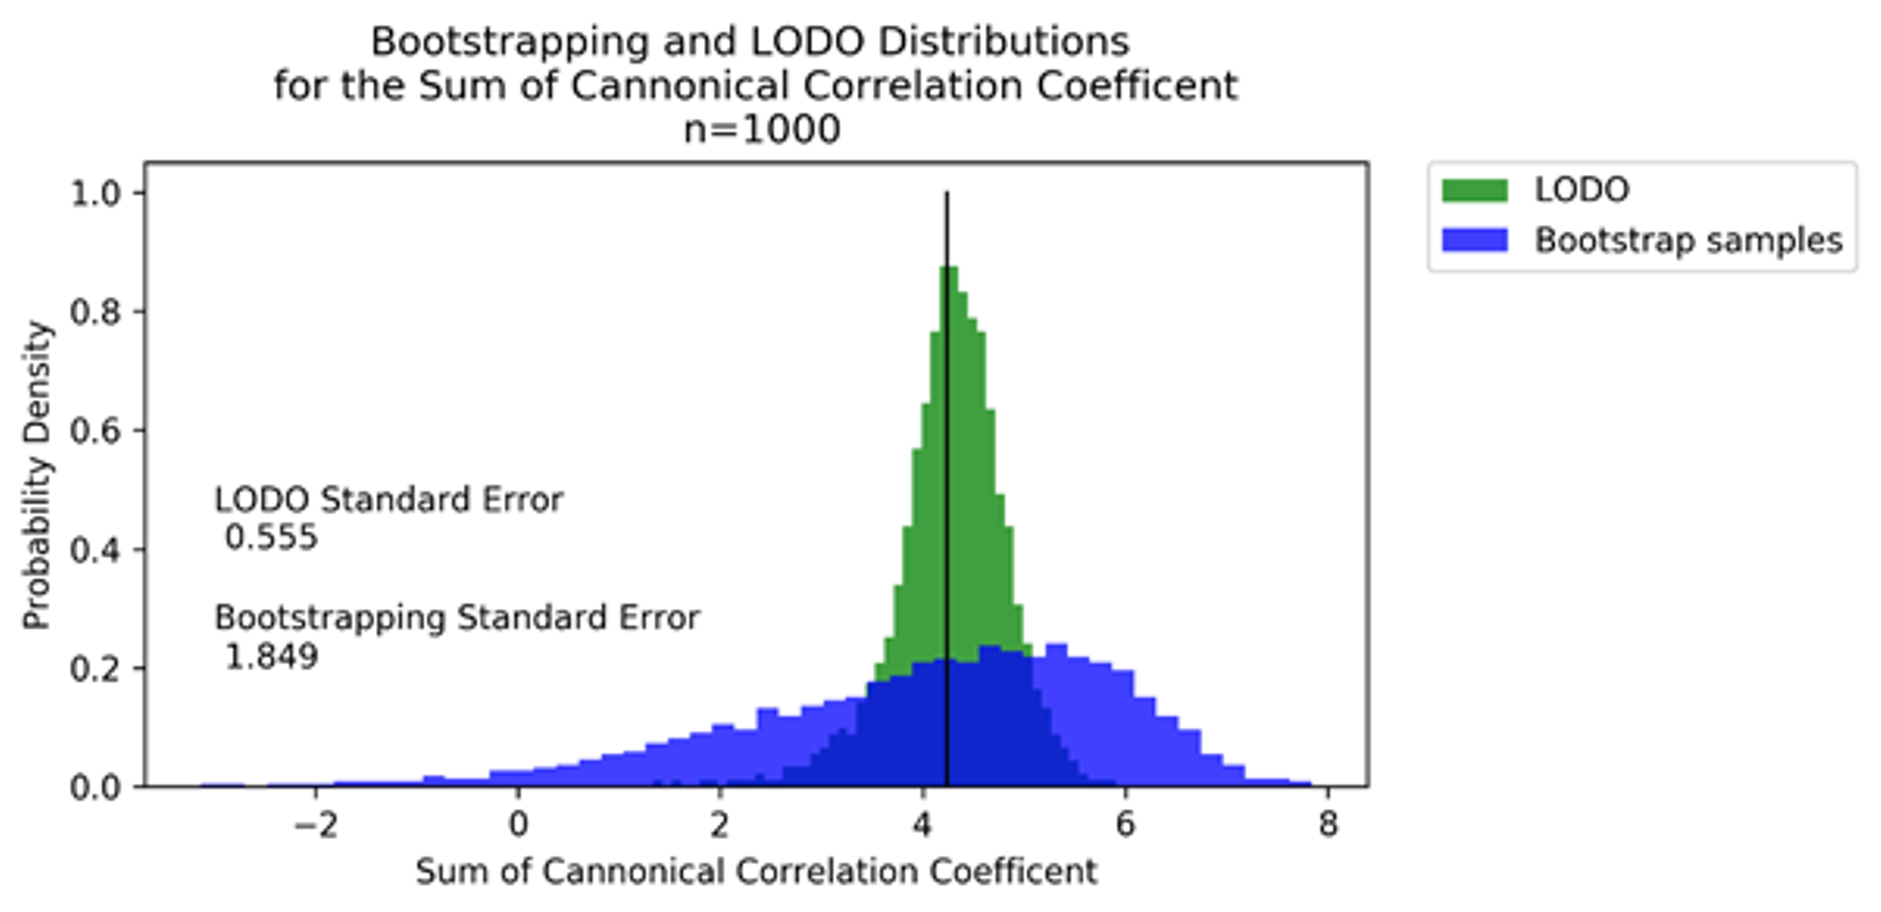
\includegraphics[width=0.8\textwidth]{chapters/img/study1figs1.png}
	\caption{Restricted temporal sampling and bootstrapping resampling distribution with 1000 iteration.} 
	\label{fig:3S1}
\end{figure}
% ==========================================================================================================
\begin{figure}[htbp]
	\centering
	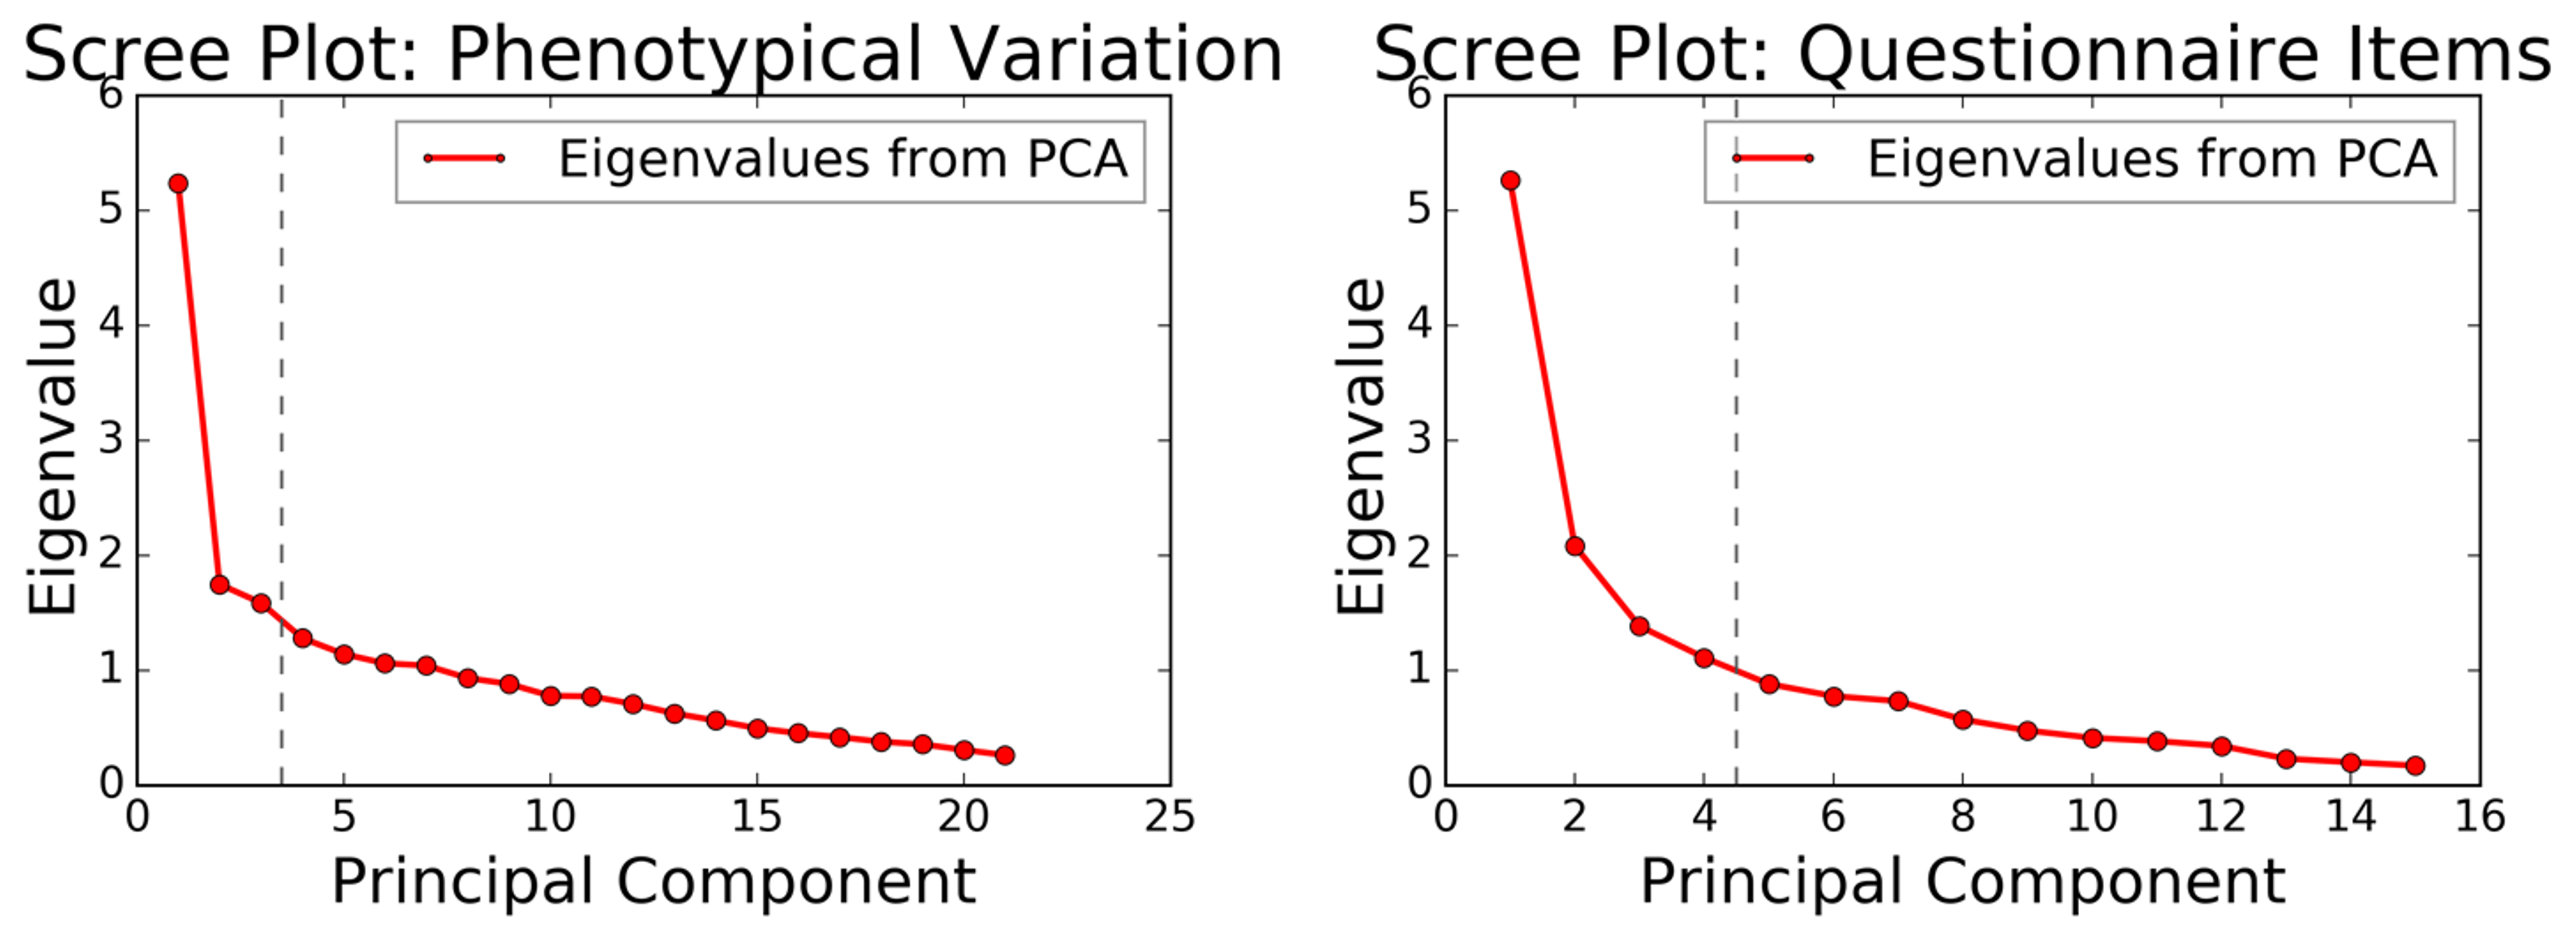
\includegraphics[width=0.8\textwidth]{chapters/img/study1figs2.png}
	\caption{Scree plots of the principle component analysis.} 
	\label{fig:3S2}
\end{figure}
% ==========================================================================================================
\begin{figure}
    See Online Supplemental Material \url{http://journals.sagepub.com/doi/suppl/10.1177/0956797617728727}
    \caption{Full set of components.} 
	\label{fig:3S3}
\end{figure}
% ==========================================================================================================
\begin{figure}
	\centering
	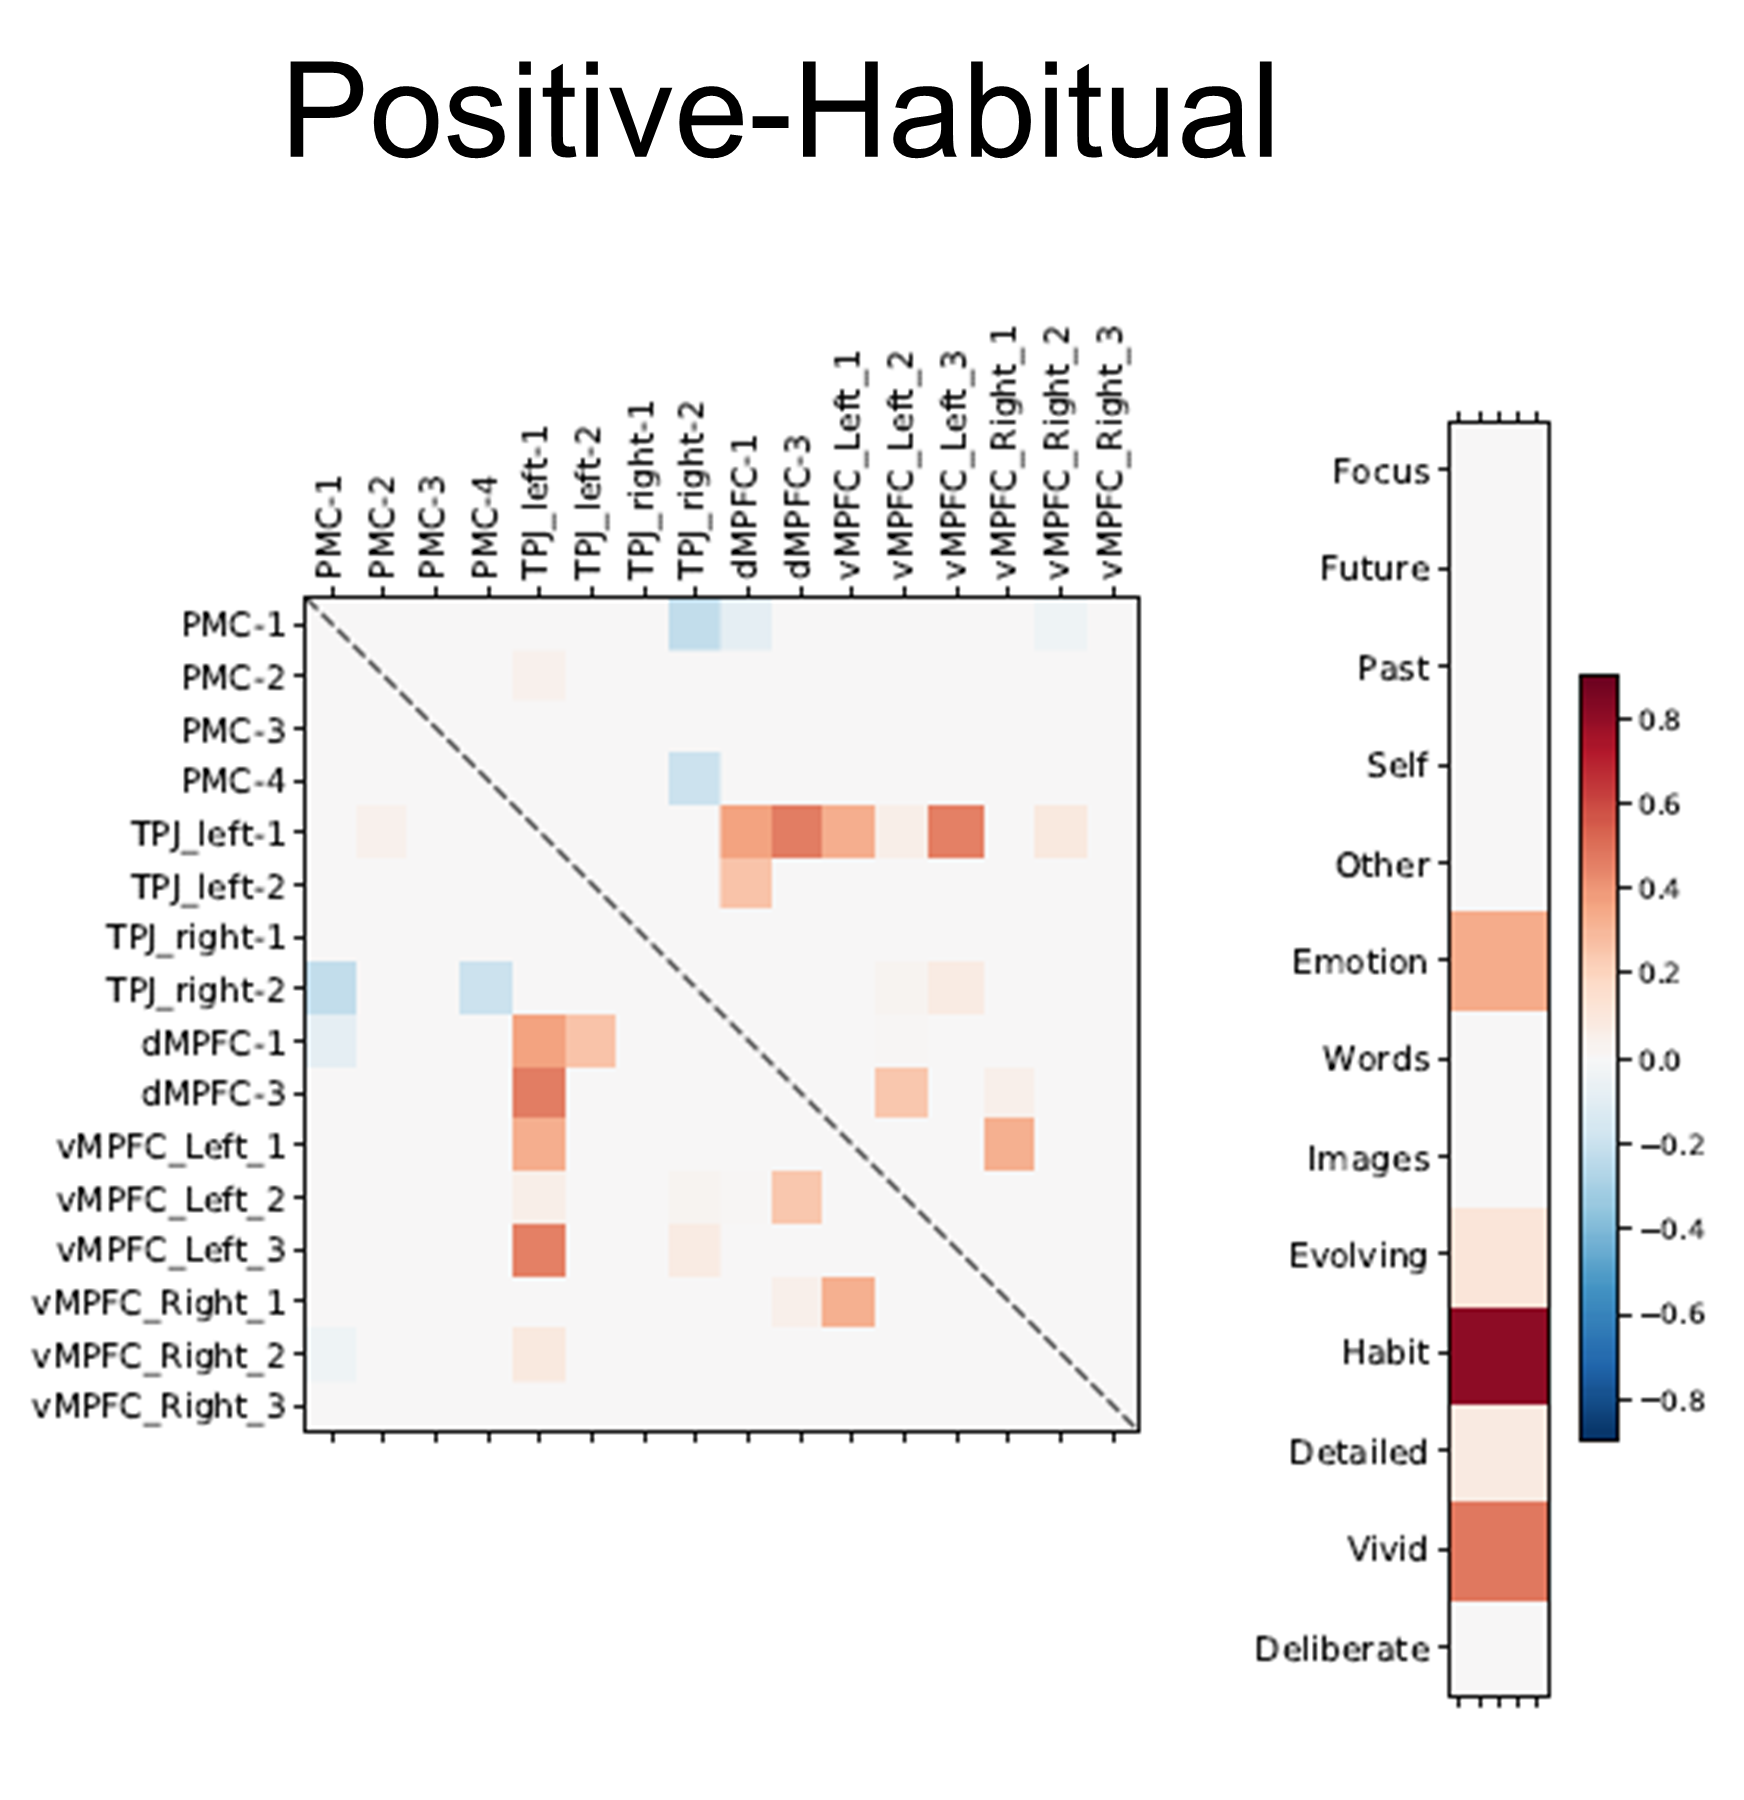
\includegraphics[width=0.6\textwidth]{chapters/img/study1figs4-1.png}
	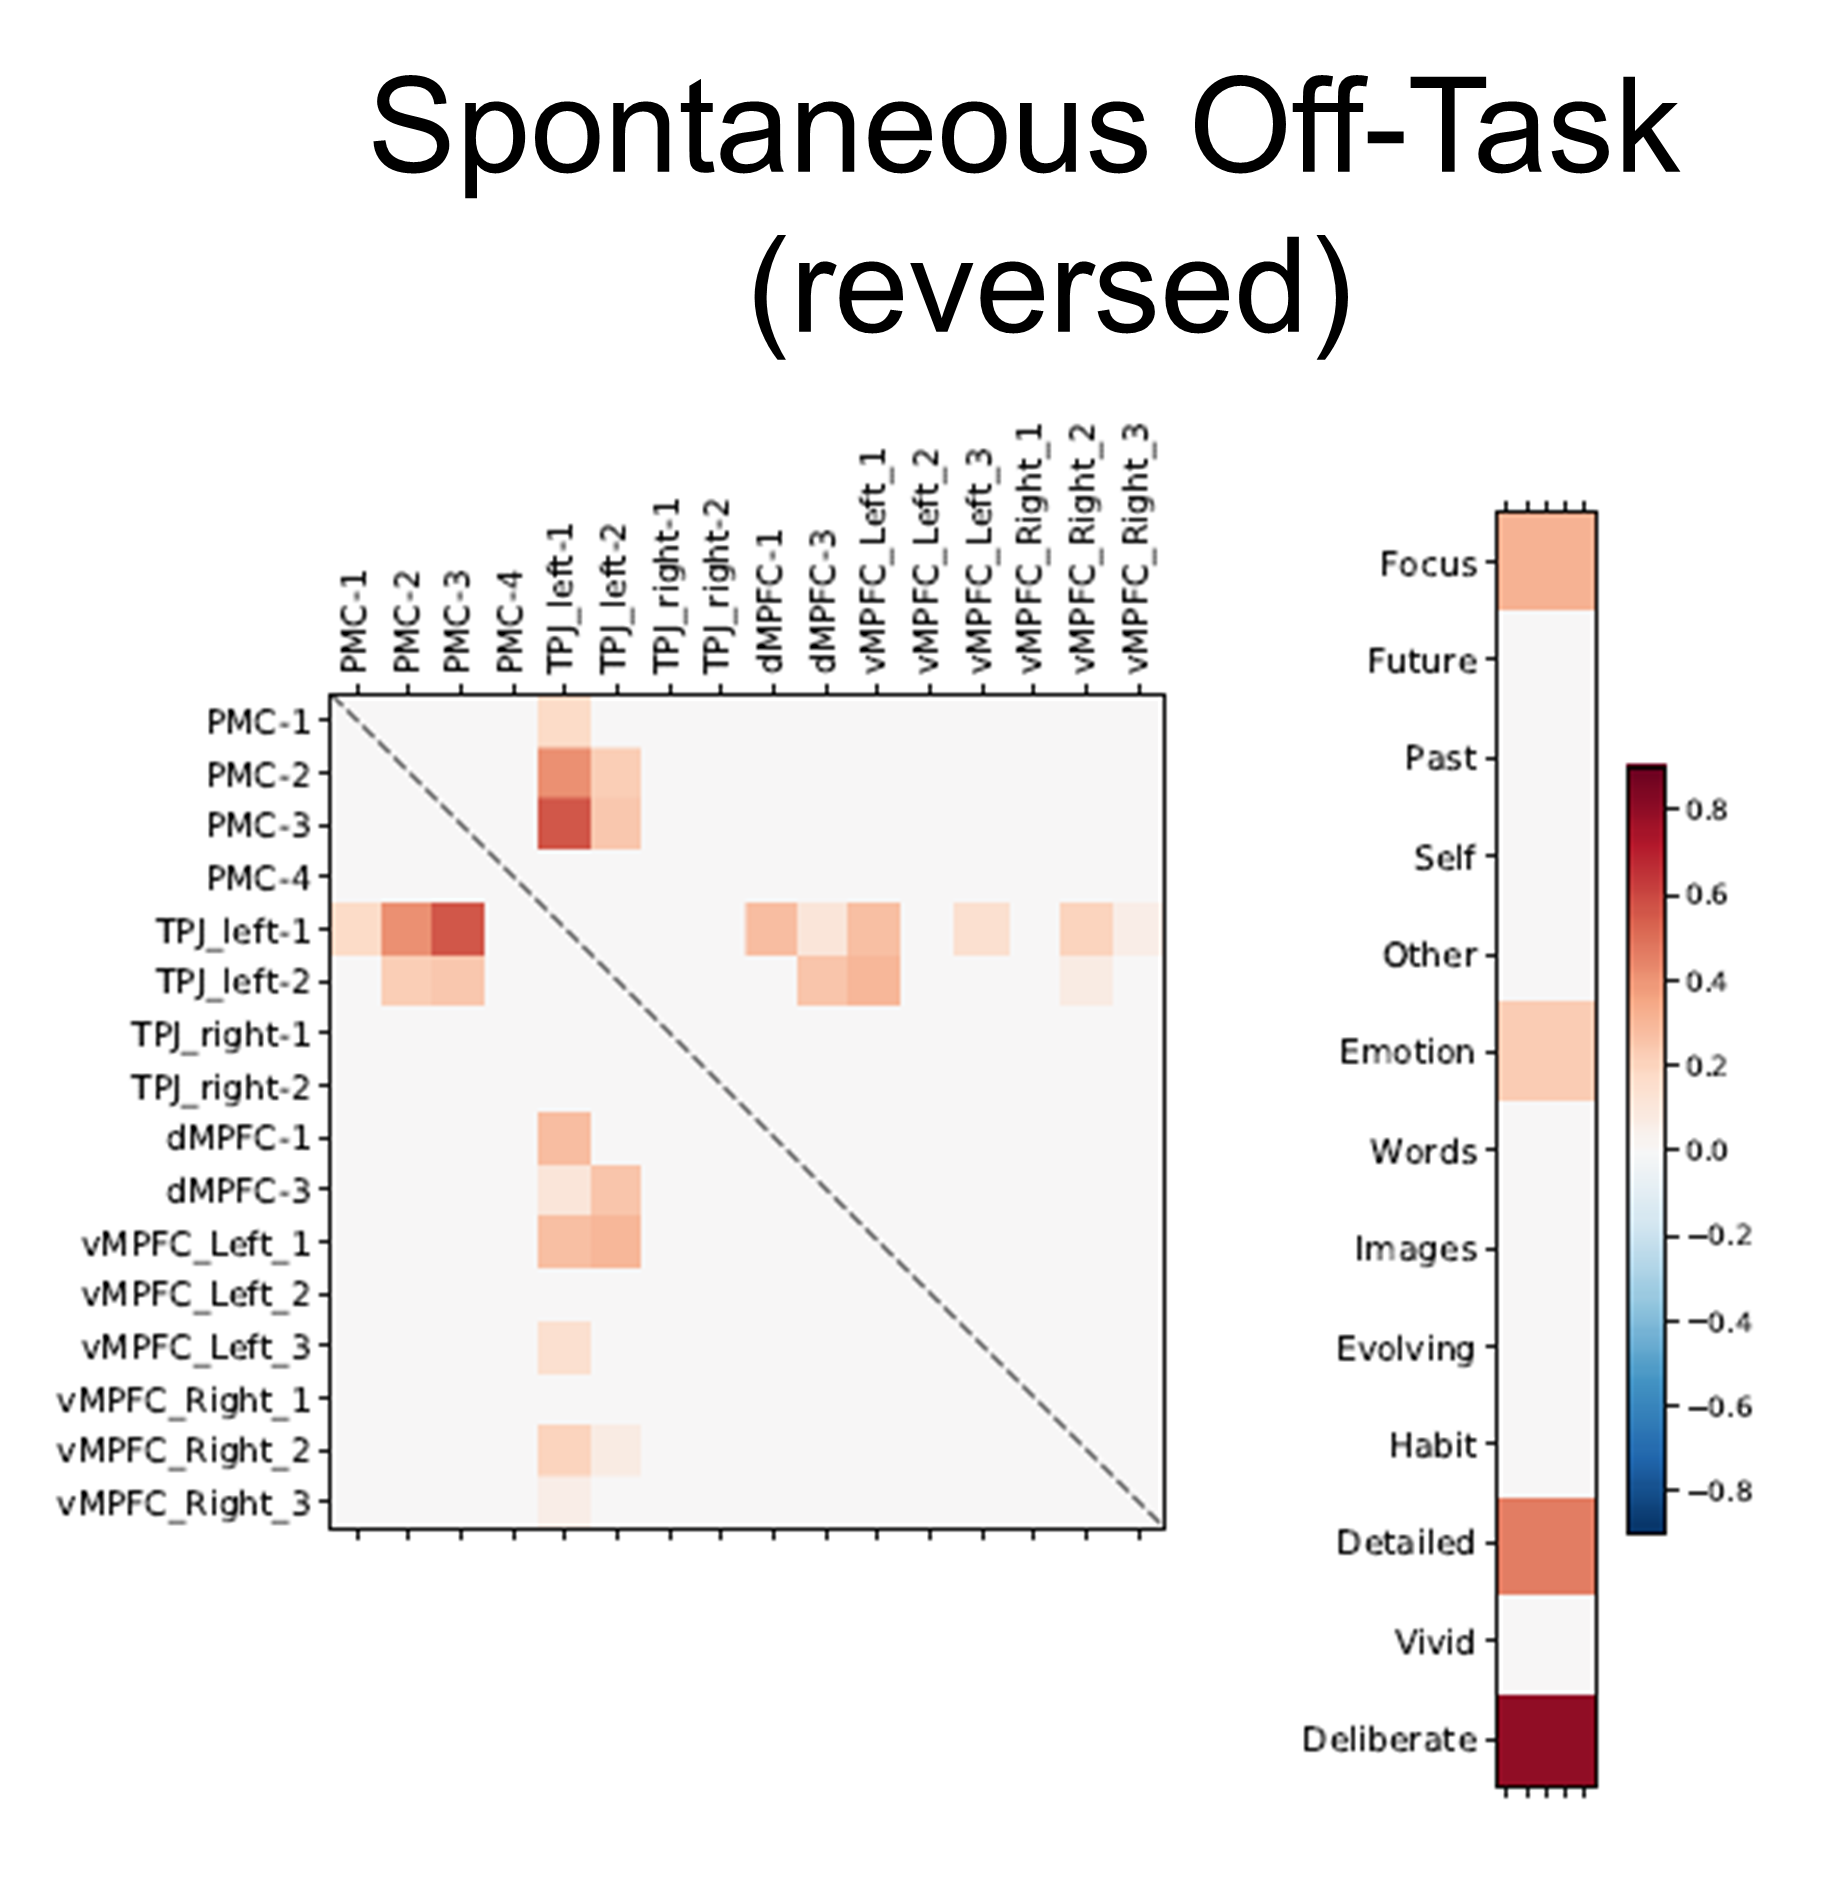
\includegraphics[width=0.6\textwidth]{chapters/img/study1figs4-2.png}
	\caption{Decomposition with motion outlier subjects excluded.} 
	\label{fig:3S4}
\end{figure}
% ==========================================================================================================
\chapter{Patterns of thought: Nested K-Fold Cross-Validation}
\label{appendix:kfold}

\linespacesmall
\begin{algorithm}[htb]\footnotesize
\begin{algorithmic}[1]
\parbox{15.0cm}
{
\FOR{\textit{Each outer fold k}} 
    \FOR{\textit{Each parameter set}} 
        \STATE Separate the development set into j folds. 
        \FOR{\textit{Each inner fold j}}  
                \STATE Train the model on the training set
                \STATE Calculate test error in the validation set j
        \ENDFOR
        \STATE Compute the average inner cross-validation test error
    \ENDFOR
    
    \STATE Choose the best parameter set with minimum average test error.
    \STATE Use this parameter set to train on the development set.
    \STATE Calculate test error in the test set
\ENDFOR
\STATE Determine the optimal model based on the outer fold test error 
\STATE Train the full dataset on the optimal model
}
\end{algorithmic}
\caption{: Nested k-fold cross-validation}
\label{algorithm:1}
\end{algorithm}
\linespacenormal

% ==========================================================================================================




% definitions and glossaries
% \cleardoublepage
% \makeabbreviations

% references
\cleardoublepage

% make my own title
\makeatletter
\let\st@rtbibsection\@bibnewpage
\let\st@rtbibchapter\@bibnewpage
\makeatother

\addcontentsline{toc}{chapter}{\numberline{}References}
\chapter*{References}
%\markboth{References}{}
\bibliographystyle{apacite}
\linespacesmall
\bibliography{thesis.bib}

% the end
\end{document}